\documentclass[12pt,titlepage]{article}
\usepackage[table]{xcolor}
\usepackage{longtable}
\usepackage[utf8]{inputenc}
%Language of Document Elements like Figure or Table
\usepackage[english]{babel}
\usepackage[bookmarks]{hyperref}
\usepackage{pdfpages}
\usepackage{graphicx}
\usepackage{float}
\usepackage{colortbl,array}
\usepackage[justification=centering]{caption}
\usepackage{enumitem}
\usepackage{chngcntr}
\usepackage{lscape}
\usepackage{fancyhdr}
\usepackage{listings}
\usepackage{hyperref}
\usepackage{nameref}
\usepackage{tabularx}
\usepackage[a4paper,width=160mm,top=25mm,bottom=25mm]{geometry}
\usepackage[ngerman]{translator}
\usepackage{acronym}
\usepackage{listings}
\usepackage{makecell}
\usepackage{rotating}


\definecolor{warningbackground}{RGB}{252,226,158}

\newcommand{\alertwarningbox}[1]{
	\begin{tabularx}{\linewidth}{
			>{\columncolor{warningbackground}}c
			>{\columncolor{warningbackground}}X}
		\raisebox{\dimexpr2\baselineskip-\height} &
		\raisebox{\tabcolsep}{\strut}#1\raisebox{-\tabcolsep}{\strut}
	\end{tabularx}
}

%Syntax-highlighting]
%\usepackage{minted}
%\usemintedstyle{vs}

%Each Section in a new Page
\let\oldsection\section
\renewcommand\section{\clearpage\oldsection}

%Set space around and between lists
\setlist[enumerate]{noitemsep, topsep=0cm}
\setlist[itemize]{noitemsep, topsep=0cm}

%Figure/Table Numbering style "Section Number.figure counter
\renewcommand{\thefigure}{\arabic{section}.\arabic{figure}}
\renewcommand{\thetable}{\arabic{section}.\arabic{table}}

%Reset figure/table counter after section change
\counterwithin{figure}{section}
\counterwithin{table}{section}

\hypersetup{
	colorlinks,
	linkcolor={black},
	citecolor={black},
	urlcolor={black}
}

\colorlet{punct}{red!60!black}
\definecolor{background}{HTML}{EEEEEE}
\definecolor{delim}{RGB}{20,105,176}
\colorlet{numb}{magenta!60!black}

\newcommand{\todonl}[1]{\newline\textcolor{red}{TODO: #1}\PackageWarning{TODO:}{#1!}}
\newcommand{\todo}[1]{\textcolor{red}{TODO: #1}\PackageWarning{TODO:}{#1!}}

%Set Paragraph indent to null
\setlength{\parindent}{0pt}
% Smaler Table Space
\renewcommand{\arraystretch}{1.5}

% renamig of section to Abschnitt \autoref
\addto\extrasenglish{%
	\def\sectionautorefname{Abschnitt}%
}

% renamig of subsubsection to Abschnitt \autoref
\addto\extrasenglish{%
	\def\subsubsectionautorefname{Abschnitt}%
}

% renamig of subsection to Abschnitt \autoref
\addto\extrasenglish{%
	\def\subsectionautorefname{Abschnitt}%
}
%rename Figure zu Abbildung
\addto\captionsenglish{\renewcommand{\figurename}{Abbildung}}

%rename Tabe zu Tabelle
\addto\captionsenglish{\renewcommand{\tablename}{Tabelle}}

% Befehle für die Tabellenerstellung der Testcases
\newcommand{\testpttb}[3]{
%	\begin{landscape}
		\subsection{#1}
		#2
		\rowcolors{2}{gray!25}{white}
		\begin{longtable}{| m{0.5cm} | m{9cm} | m{6cm} | m{6cm} | m{1.5cm} |}
			\hline
			\textbf{Nr} & \textbf{Beschreibung} & \textbf{Erwartetes Ergebnis} & \textbf{Tatsächliches Ergebnis} & \textbf{Status}
			\\
			\hline
			#3
			\hline
		\end{longtable}
%	\end{landscape}
}

\newcommand{\testptrow}[5]{
	#1 & #2 & #3 & #4 & #5 \\
}

\title{Software-Defined Netzwerk im Campus Bereich}
\author{Sandro Kaspar, Philipp Albrecht, Jessica Kalberer}
\date{28.02.2017}

\pagestyle{fancy}
\lhead{Software-Defined Netzwerk im Campus Bereich}
\begin{document}
\pagenumbering{Roman}



\includepdf{pdfincludes/titlepage}

\newpage
%new Title for tableofcontent
\renewcommand{\contentsname}{Inhaltsverzeichnis}
\tableofcontents
\newpage
\pagenumbering{arabic}

\section{Aufgabenstellung}
Dies ist die initiale Aufgabenstellung, welche zu Beginn der Studienarbeit vorlag. 

\begin{figure}[H]
	\centering
	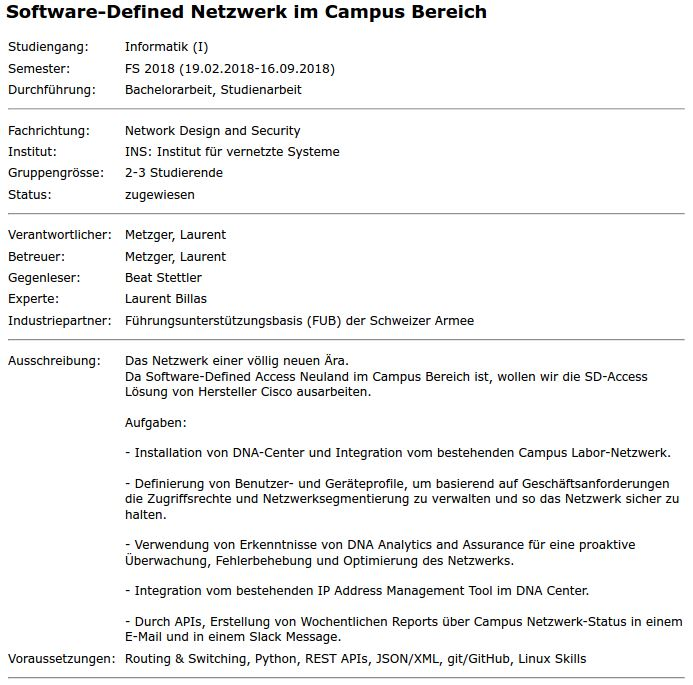
\includegraphics[height=16cm]{img/aufgabenstellung.jpg}
	\caption{Aufgabenstellung aus AVT \cite{avt-tool}}
	\label{fig:Aufgabenstellung}
\end{figure}

Die Zielsetzungen der initialen Aufgabenstellung wurden nach Absprache mit dem Betreuer anhand der Erkentnisse im Verlauf der Studienarbeit angepasst. Die aktualisierte Aufgabenstellung mit den dazugehörigen Zielsetzungen sind im Abstract ersichtlich (Siehe: \ref{Abstract} Aufgabenstellung).

\section{Abstract}
Der Abstract richtet sich an den Spezialisten auf dem entsprechenden Gebiet und 
beschreibt daher in erster Linie die (neuen, eigenen) Ergebnisse und Resultate der 
Arbeit. Es umfasst nie mehr als eine Seite, typisch sogar nur etwa 200 Worte (etwa 
20 Zeilen). Es sind keine Bilder zu verwenden.

\subsection{Version 2}

Ziel dieser Studienarbeit war die Evaluation des Cisco Digital Network Architecture (DNA) Center, der Software Defined Access Lösung von Cisco, für die Führungsunterstützungsbasis der Schweizer Armee. Der erste Schwerpunkt lag dabei auf der Installation des DNA Centers und der Konfiguration sowie Integration eines Campus Netzwerkes. Für das DNS-, DHCP- und IP-Adress-Management (IPAM) wird im Campus Netzwerk Infoblox eingesetzt. Für die Benutzerverwaltung sowie Zugriffskontrolle wird die Cisco Identity Services Engine (ISE) verwendet.

Nach dem Einrichten des Campus Netzwerkes lag der zweite Schwerpunkt auf der Definition von Benutzer- und Geräteprofilen, um den einzelnen Mitarbeitern der Schweizer Armee den Netzwerkzugriff zu ermöglichen und die Zugriffsrechte der einzelnen Mitarbeiter oder eines Teams zentral zu regeln. Des Weiteren sollte mit DNA Assurance eine proaktive Überwachung, Fehlerbehebung und Optimierung des Netzwerkes sichergestellt werden. Mit diesen Informationen sollten wöchentliche Reports über den Status des Netzwerks per E-Mail oder Slack Message versendet werden.\\
\\
Die Inbetriebnahme des Campus Netzwerkes gestaltete sich schwieriger als erwartet. Viele der Schritte sind nur teilweise automatisiert und es ist sehr viel manueller Aufwand nötig. Als Beispiel kann hier die LAN Automation aufgeführt werden. Mit Hilfe dieser sollten sich Netzwerkgeräte automatisiert via PnP in Betrieb nehmen und konfigurieren lassen. Dieser Prozess ist allerdings sehr fehleranfällig und funktioniert nur unzuverlässig, sodass die Inbetriebnahme des Underlay Netzwerkes erst nach mehreren Versuchen korrekt ausgeführt werden konnte. 
Des Weiteren funktionieren viele Funktionen des DNA Centers nur mit spezifischen Versionen von ISE und IOS-XE. Dies führte zu weiteren Komplikationen, da dies vom Hersteller so nicht dokumentiert ist. 
Durch diese Komplikationen wurde der ganze Provisionierungsprozess verzögert. 
\\
Abschliessend kann gesagt werden, das für die Installation und Konfiguration des DNA Centers mehrere Tage, wenn nicht Wochen eingerechnet werden müssen. Zudem muss im optimalen Fall ein Green Field vorliegen, da zur Zeit kein bestehendes Netzwerk ohne Unterbrüche migriert werden kann. Bei der Installation sollten die empfohlenen Softwareversionen genauestens eingehalten werden, da sonst die volle Funktionalität des DNA Centers nicht gewährleistet werden kann. Beim Kauf des DNA Centers ist es am einfachsten, gleich auch einen Experten von Cisco aufzubieten, um diese Appliance komplett in der gewünschten Umgebung in Betrieb zu nehmen. 

%\subsection{Ausgangslage}

%\subsection{Ziele der Arbeit}
%Das grundsätzliche Ziel ist eine Evaluation des Cisco Software Defined Networking. Im ersten Schritt beinhaltet das die %Inbetriebnahme und Konfiguration von den folgenden Komponenten:
%\begin{itemize}
%	\item Cisco DNA Center Appliance
%	\item Integration Infoblox (One Platform Solution für DNS, DHCP, IPAM)
%	\item Integration Cisco ISE (Access and Authentification Control)
%	\item Integration Campus Labor Netzwerk
%\end{itemize}
%Im zweiten Schritt sollen UseCases durchgespielt werden, die den folgenden Umfang abdecken:
%\begin{itemize}
%	\item Definierung von Benutzer- und Geräteprofile, um basierend auf Geschäftsanforderungen die Zugriffsrechte und Netzwerksegmentierung zu verwalten und so das Netzwerk sicher zu halten.
%	\item DNA Analytics and Assurance für eine proaktive Überwachung, Fehlerbehebung und Optimierung des Netzwerks.
%	\item IP Address Management Tool im DNA Center.
%	\item Wöchentliche Reports über Campus Netzwerk-Status via E-Mail oder Slack
%\end{itemize}

%\subsection{Ergebnisse}

\section{Management Summary}

\subsection{Ausgangslage}
Diese Arbeit beschäftigt sich mit Software Defined Networking im Campus LAN für die Führungsunterstützungsbasis der Schweizer Armee. Die Lösung soll den Netzwerkzugriff der Mitarbeiter der FUB sicherstellen und die Zugriffsrechte der einzelnen Mitarbeiter oder Teams regeln können. 
Des Weiteren müssen Reportingfunktionion und eine proaktive Überwachung erstellt werden, um allfällige Fehler schnellstmöglich zu erkennen, das Netzwerk stets zu optimieren und dessen Funktion jederzeit sicherzustellen.
Zusätzlich wird ein bestehends IP Management Tool in die Lösung integriert.

Da die Anforderungen an Campus Netzwerke aus verschiensten Gründen, wie z.Bsp. modernen Arbeitsmodellen, neuen Sicherheitsanforderungen usw. ständig steigen, ist es äusserst schwierig und aufwändig, diese Anforderungen mit traditionellen Methoden zu erfüllen. 

Um dies zu erreichen, wird in dieser Arbeit daher ein Software Defined Network erstellt, dass diesen neuen Anforderungen gerecht werden soll. Vorteile zeigen sich insbesondere dadurch, dass eine derartige Lösung flexibler ist, also einfacher und schneller an neue Gegebenheiten angepasst werden kann und durch Schnittstellen einfach an bestehende Systeme anzubinden ist. Durch das zentrale Management und Monitoring der Komponenten sinkt zudem das Risiko für Fehler massiv und viele Aufgaben lassen sich einfach und schnell automatisieren.
Schlussendlich kann durch diese Vorteile sehr viel Aufwand und damit Kosten eingespart werden.

Ziel ist es, die Vorteile dieser Lösung gegenüber einer traditionellen Netzwerkinfrastruktur aufzuzeigen, allfällige Risiken und mögliche Probleme früh zu erkennen und Lösungen für diese zu finden. 
\subsection{Vorgehen und Technologien}
Die Lösung wird mit dem Produkt Software Defined Access von Cisco erstellt. Diese besteht aus mehreren Komponenten dies ist zum einem das DNA Center, welches die grundsätzliche Funktion des Netzwerks sicherstellt, sowie ISE (Identity Service Engine), welches die Benutzeridentitäten und Profile verwaltet.
Zusätzlich muss das bestehende IP Management in die Lösung integriert werden und Reporting Funktionen mittels Slack und E-Mail implementiert werden. Diese Zusatzfunktionalitäten werden in Python implementiert und nutzen die in Ciscos SDA enthaltenen APIs.
\subsection{Ergebnisse}
Am Ende dieser Arbeit wird ein funktionierender Prototyp eines Software Defined Networks im Access Bereich zur Verfügung stehen, der alle Requirements des Industriepartners abdeckt. Der Prototyp besteht aus den Cisco Komponenten, sowie Eigenentwicklungen, die zusätzliche Features implementieren. 
Zudem steht eine Dokumentation des Systems zur Verfügung, die den Installationsprozess und die Handhabung des Systems erklärt. Des Weiteren zeigt die Dokumentation Vorteile, aber auch Risiken und mögliche Probleme im Vergleich zu einer traditionellen Netzwerklösung auf.
\subsection{Ausblick}
Die Resultate aus dieser Arbeit können dazu dienen, SDA in einer produktiven Umgebung in Betrieb zu nehmen. Zudem kann er Prototyp um zusätzliche Funktionen erweitert werden, an zusätzliche bestehende oder neue Systeme angebunden werden oder mit alternativen Lösungen verglichen werden.

\section{Ausgangslage (Kontext)}

\begin{itemize}	
	\item Beschreibung des Typs der Arbeit (Bsp. Fokus Lösungserstellung oder Machbarkeitsanalyse)
	\item Fachliche Domäne, Zielgruppe, heutige Praktiken bzw. Lösungen (Methoden, Tools, etc.)
\end{itemize}


\section{Problembeschreibung (Stand der Technik)}

\begin{itemize}	
	\item Motivation für die Arbeit, z.B. aus den Schwächen der heutigen Praktiken bzw. Lösungen
	\item Funktionale Anforderungen beschrieben (z.B. als Use Cases (short) mit Aktoren oder in Form von User Stories mit Personas)
	\item Wichtigste NFA/Qualitätsattribute abgedeckt und überprüfbar beschrieben
\end{itemize}

Um den heutigen Anforderungen an Campus Netzwerke im Bezug auf Sicherheit, Wartbarkeit und Skalierbarkeit gerecht zu werden, steht man mit der isolierten Konfiguration einzelner Komponenten schnell vor verschiedenen Problemen. In erster Linie ist es extrem Aufwändig alle Konfigurationen manuell zu erstellen. Selbst das Hinzufügen von einfachen Richtlinien oder zum Beispiel neuen Firmenabteilungen können zu gewaltigem Aufwand führen. Des weiteren verliert man schnell die Übersicht und ist gezwungen umfangreiche Dokumentationen zu erstellen. Häufig kommen selbstgeschriebene Scripts zum Beispiel mithilfe von NAPALM (Siehe: \cite{napalm}) zur automatisierten Konfiguration zum Einsatz. Für das Monitoring des Netzwerkes sind zusätzlich Tools wie icinga2  (Siehe: \cite{icinga2}) oder ähnliches nötig. 

~\\
Typische Herausforderungen bei den klassischen Campus Netzwerken:
\begin{itemize}
	\item Zu wenig VLAN
	\item VLAN über ein Layer 3 Netzwerk
	\item Mobilität von Komponenten
	\item Mobilität von Benutzer (Netzwerk Teilnehmer)
	\item Durchsetzen von Sicherheitsregeln mithilfe von Firewalls
	\item Direkte Abhängigkeit von Berechtigungen und IP Subnetzen
	\item Mehrere Unabhängige Tools mit Informationsredundanz
	\item Komplexe Fehlersuche über verschiedene Komponenten/Geräte hinweg.
\end{itemize}

~\\
Genau hier setzt das Cisco DNA Center an. Es fasst alle diese Tools unter einem Dach zusammen und bietet eine übergreifende Plattform. 


\section{Lösungskonzept}

\begin{itemize}	
	\item Dokumentation Architektur und Design (i.d.R. plattformneutral bzw. technologieübergreifend, z.B. in Form von UML-Diagrammen und Erläuterungen dazu) 
	\item Architekturentscheidungen mit Begründungen
	\item Diskussion, wie Qualitätsattribute adressiert werden (welche Qualität kann erreicht werden?)
\end{itemize}


\begin{figure}[H]
	\centering
	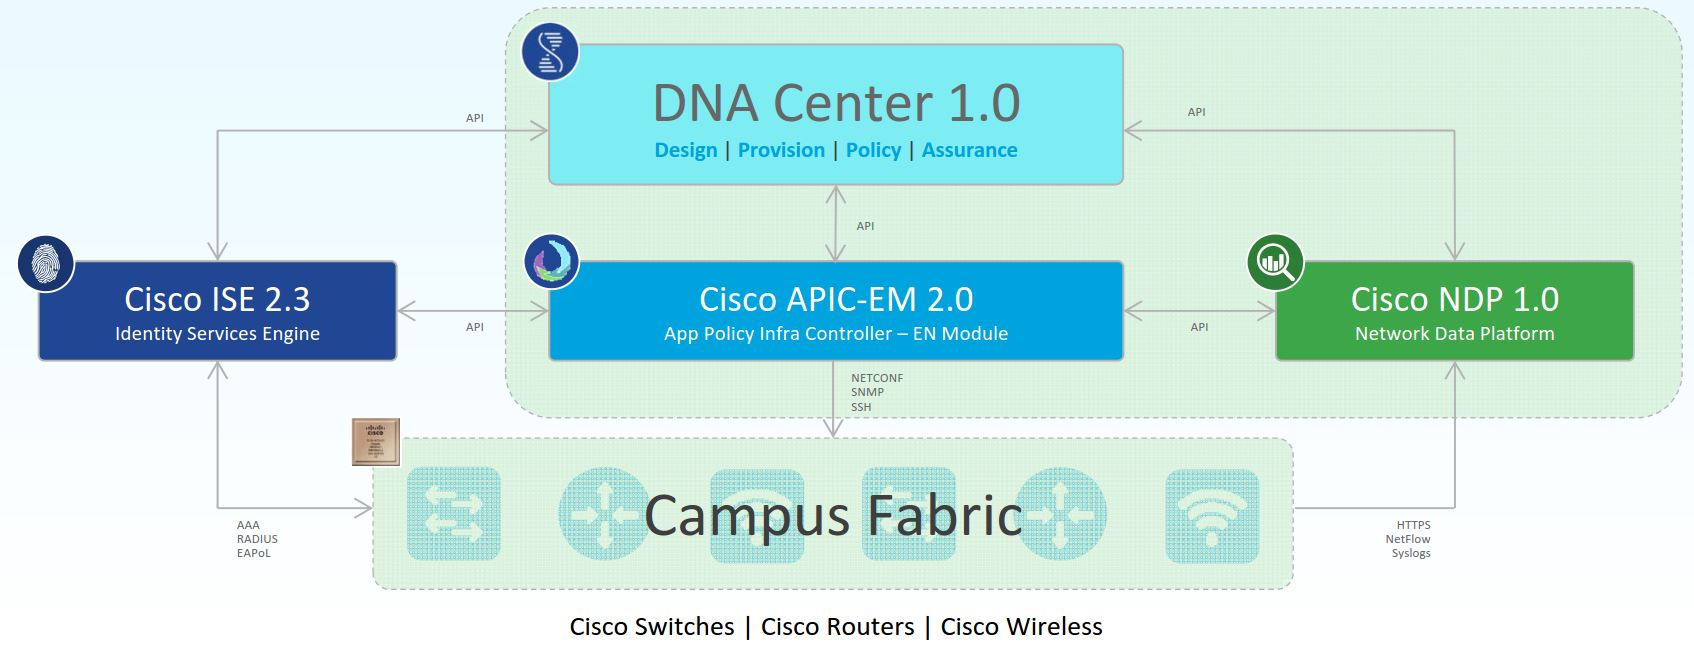
\includegraphics[height=6.3cm]{img/DNAC-Components.jpg}
	\caption{DNAC Komponenten}
	\label{fig:DNAC Komponenten}
\end{figure}

\section{Technologien}

\subsection{Software Defined Access (SDA)}
Cisco bietet mit SDA eine automatisierte End-to-End-Segmentierung um den Benutzer-, Geräte- und Anwendungsverkehr zu trennen, ohne das Netzwerk neu zu gestalten. Durch diesen automatisierten Benutzerzugriff ermöglicht SDA Einrichtungen innert kürzester Zeit. Durch diese enorme Vereinfachung wird eine zusätzliche Sicherheit und Skalierung des Betriebs gewonnen. Ebenso wird die Transparenz deutlich erhöht und die schnelle Bereitstellung neuer Dienste gewährleistet. Durch die Automatisierung von täglichen Aufgaben wie Konfiguration, Bereitstellung und Troubleshooting reduziert SDA die Zeit für Netzwerkanpassungen, verbessert die Problemlösungszeit und reduziert die Auswirkungen von Sicherheitsverletzungen.\\
\\
So können Organisationen sicherstellen, dass für jeden Benutzer oder jedes Gerät mit jeder Anwendung die richtigen Richtlinien festgelegt werden über das Netzwerk. Dies wird mit einer einzigen Netzwerkstruktur über LAN und WLAN erreicht, wodurch ein konsistente Benutzererfahrung überall ohne Kompromisse bei der Sicherheit. \\
\\
SDA wird aus mehreren Komponenten zusammengesetzt. Dazu gehört das DNA-Center, welches die grundsätzliche Funktion des Netzwerks sicherstellt, sowie Identity Service Engine (ISE), welches die Benutzeridentitäten und Profile verwaltet.
\footnote{SDA Cisco Definition: https://www.cisco.com/c/en/us/solutions/enterprise-networks/software-defined-access/index.html}

\subsubsection{Campus Fabric}
Um eine konsistente Benutzererfahrung zu erreichen, braucht man eine Switching-Infrastruktur mit der sich der Zugang zu bestimmten IP-Subnetzen ortsunabhängig realisieren lässt.

Cisco hat nun ein neues Overlay für diesen Zweck erfunden, die "Campus Fabric". Das Overlay ist hierbei eine Kombination aus LISP und VXLAN. \footnote{Campus Fabric: https://www.cisco.com/c/dam/m/hr\_hr/training-events/2017/cisco-connect/pdf/Cisco-Campus-Fabric-Introduction.pdf}

\begin{figure}[H]
	\centering
	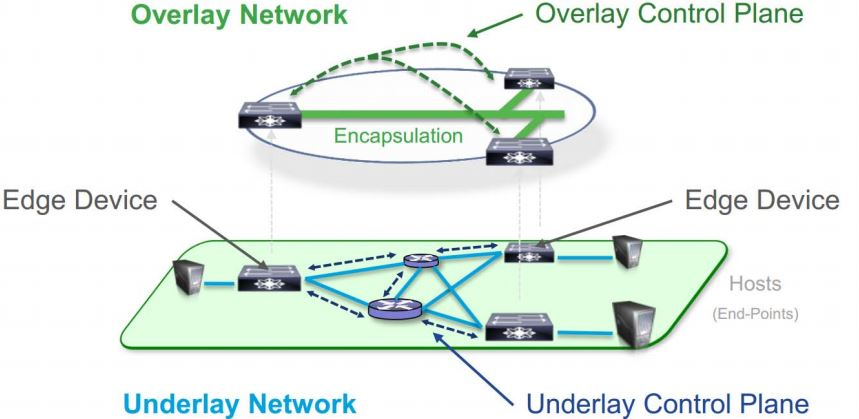
\includegraphics[height=6cm]{img/campusfabric.jpg}
	\caption{Campus Fabric}
	\label{fig:Campus Fabric}
\end{figure}

Die Fabric bildet ein Overlay Netz. Das Overlay Netz bildet eine virtuelle Topologie um Geräte miteinander zu verbinden, welches auf einer beliebigen physischen Underlay Topologie aufgebaut ist. Das Overlay Netzwerk verwendet oft alternative Weiterleitungsattribute, um zusätzliche Dienste bereitzustellen, die nicht vom Underlay Netzwerk bereitgestellt werden.

In der nachfolgenden Abbildung ist der Aufbau eines Campus Fabric etwas detaillierter aufgezeigt.

\begin{figure}[H]
	\centering
	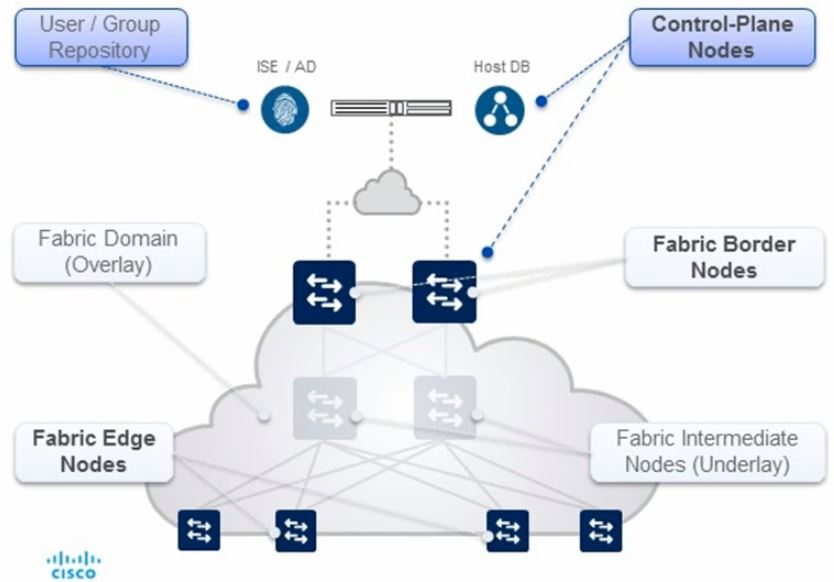
\includegraphics[height=8cm]{img/fabric-roles&terminology.jpg}
	\caption{Fabric Rollen und Terminologie}
	\label{fig:Fabric Rollen und Terminologie}
\end{figure}

Dieses Campus Fabric besteht aus folgenden Elementen:
\begin{itemize}	
	\item User/Group Repository: Ein externes ID-Speichergerät (z. B. ISE oder AD) kann verwendet werden, um eine dynamische Zuordnung von Benutzer/Gerät zu Gruppen bereitzustellen
	\item Control-Plane-Nodes: Ein Map System, das die Beziehung eines Endpoints zu einem Gateway (Edge oder Border) verwaltet
	\item Border-Nodes: Das L3-Gateway-Gerät (Core), das externe L3-Netzwerke mit dem Fabric verbindet
	\item Edge-Nodes: Das L3-Gateway-Gerät (Access oder Distribution), das Endpoints mit Fabric verbindet
	\item Intermediate Nodes: Normale L3 (IP) Forwarder im Underlay Netzwerk
\end{itemize}

\subsection{Cisco Digital Network Architecture Center (Cisco DNA-Center)}
DNA Center ist das zentrale Überwachungs-Dashboard für Netzwerke, mit dem alle Cisco DNA-Produkte und -Lösungen verwaltet werden können.
DNA Center gibt die Möglichkeit unter einem Grafischen Nutzer Interface direkt mit APIC(Application Policy Infrastructure Controller)-EM 2.x Applikationen mit der Identity Services Engine (ISE) und mit Network Data Plattform (NDP) unserer Assurance und Analytics Plattform zu sprechen. Alle Parameter die angezeigt oder konfiguriert werden müssen kann man unter DNA Center ausführen und muss nicht zwischen den einzelnen Modulen und Oberflächen hin und her springen.
\begin{figure}[H]
	\centering
	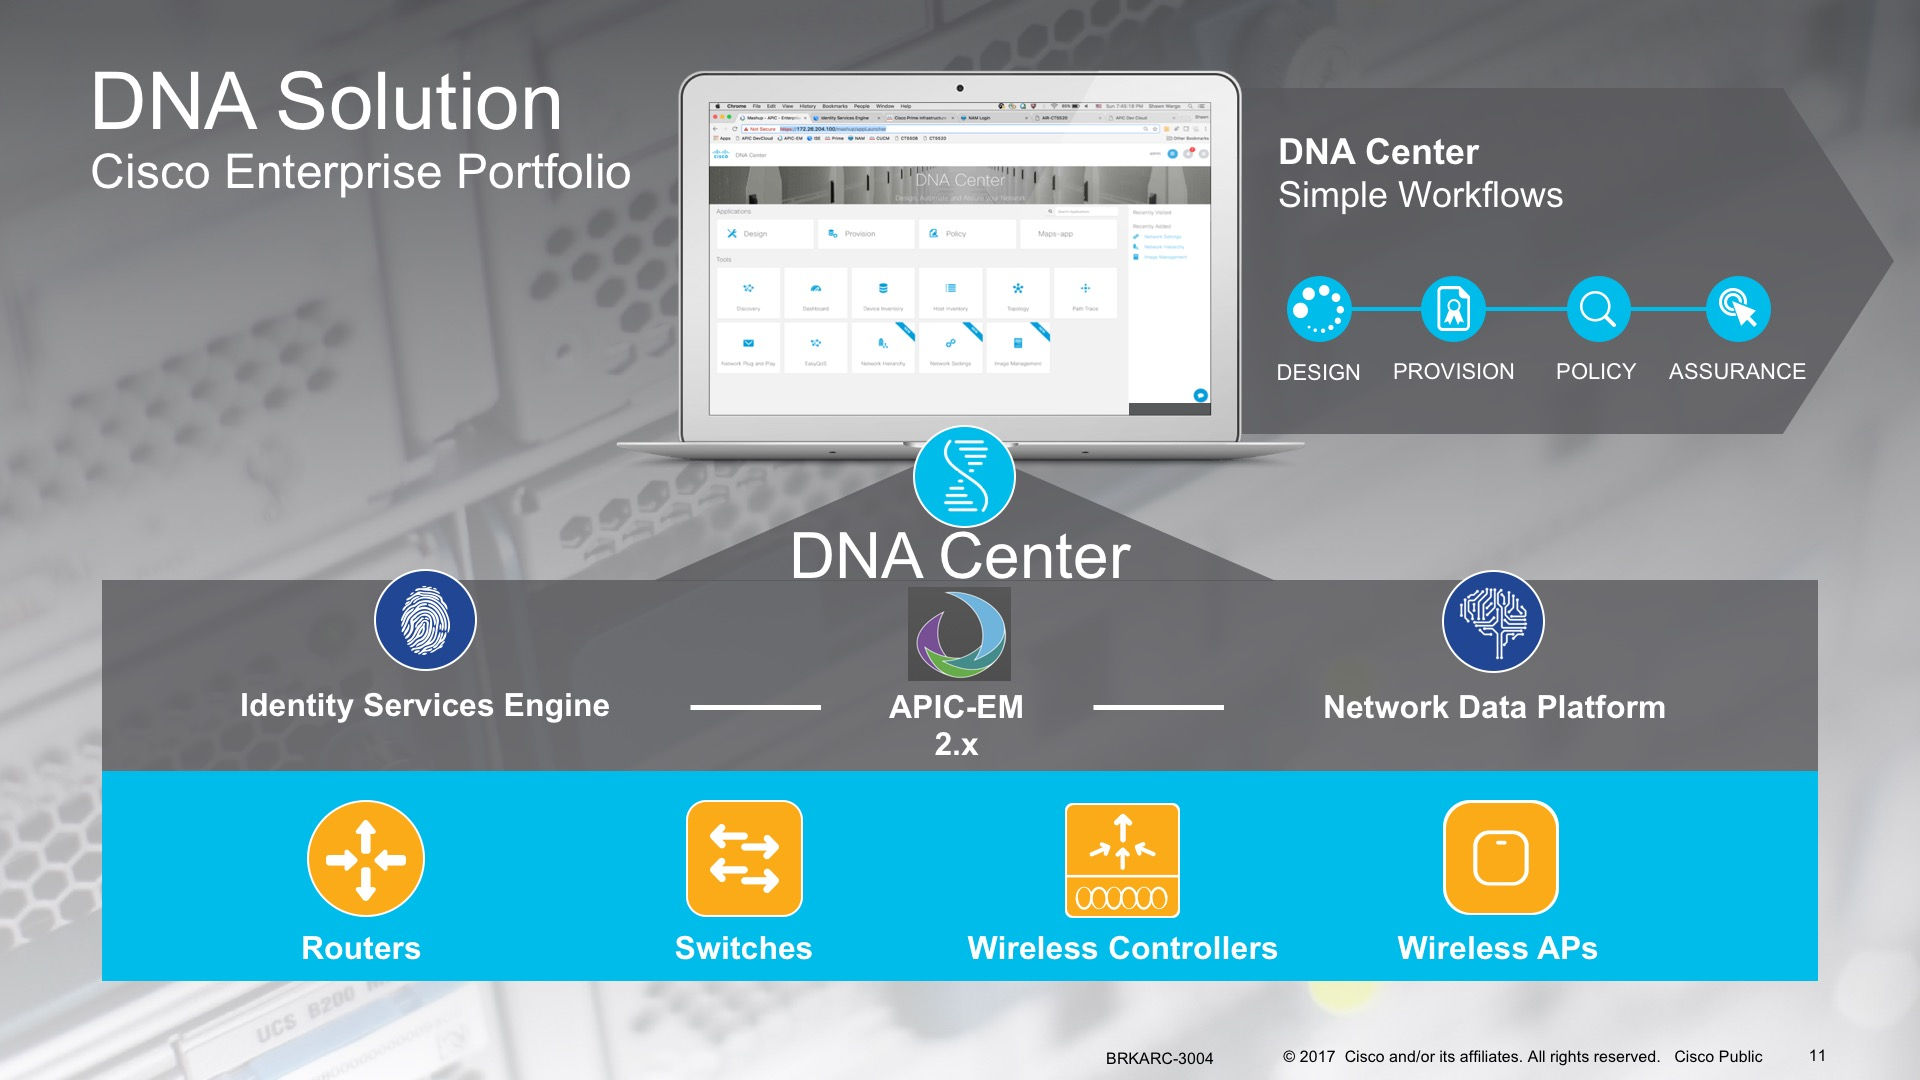
\includegraphics[height=7cm]{img/DNAC-1.jpg}
	\caption{DNA Solution}
	\label{fig:Aufbau einer DNA Solution}
\end{figure}
APIC-EM 2.x automatisiert dann die notwendigen Konfigurationen und spricht mit dem Netzwerk. Auch die Integration von IP Address Management Lösungen wie zB Infoblox werden nur über die DNA Center Oberfläche konfiguriert. \\
\\
SD-Access ist die Grundlage von Cisco DNA. Es ermöglicht Netzwerkzugriff in Minuten für jeden Benutzer oder jedes Gerät für jede Anwendung, ohne Kompromisse. Bei SD-Access folgen die festgelegten Richtlinien automatisch dem Benutzer über alle Netzwerkdomänen hinweg.

\subsection{Identity Service Engine (ISE)}
Mit der Cisco ISE können Benutzer und Geräte, die mit dem Unternehmensnetzwerk verbunden sind, angezeigt und gesteuert werden. Das alles von einer zentralen Stelle aus. ISE ermöglicht es einem Netzwerkadministrator, Zugriffsrichtlinien für kabelgebundene und drahtlose Endpunkte basierend auf Informationen zentral zu steuern, die über RADIUS-Nachrichten gesammelt werden, die zwischen dem Gerät und dem ISE-Knoten übertragen werden. Dies wird auch als Profiling bezeichnet. Die Profiling-Datenbank wird regelmäßig aktualisiert, um mit den neuesten und besten Geräten Schritt zu halten, so dass keine Lücken in der Gerätesichtbarkeit bestehen. \\
\\
Im Wesentlichen hängt ISE eine Identität an ein Gerät an, basierend auf Benutzer-, Funktions- oder anderen Attributen, um Richtliniendurchsetzung und Sicherheitskonformität bereitzustellen, bevor das Gerät autorisiert wird, auf das Netzwerk zuzugreifen. Basierend auf den Ergebnissen einer Vielzahl von Variablen kann ein Endpunkt mit bestimmten Zugriffsregeln auf das Netzwerk zugelassen werden, die auf die Schnittstelle angewendet werden, mit der er verbunden ist. Andernfalls kann er vollständig verweigert oder basierend auf den spezifischen Unternehmensrichtlinien gewährt werden. \\
\\
DNA Center bietet einen Mechanismus zum Erstellen einer vertrauenswürdigen Kommunikationsverbindung mit Cisco Identity Services Engine (ISE) und ermöglicht den beiden Anwendungen, Daten auf sichere Weise miteinander zu teilen. Sobald die ISE beim DNA Center registriert ist, wird jedes Gerät, das ISE entdeckt, zusammen mit der entsprechenden Konfiguration und anderen Daten an das DNA Center weitergeleitet. Benutzer können beide Anwendungen verwenden, um Geräte zu erkennen und dann sowohl DNA Center- als auch ISE-Funktionen auf sie anzuwenden, da diese Geräte in beiden Anwendungen verfügbar sind. DNA Center- und ISE-Geräte werden alle durch ihre Gerätenamen eindeutig identifiziert. \\
\\
In ähnlicher Weise werden DNA-Center-Geräte, sobald sie bereitgestellt werden und zu einer bestimmten Site in der DNA Center-Standorthierarchie gehören, an ISE übergeben. Alle Aktualisierungen an einem DNA Center-Gerät (z. B. Änderungen an der IP-Adresse, SNMP- oder CLI-Anmeldeinformationen, gemeinsamer ISE-Schlüssel usw.) werden automatisch an die entsprechende Geräteinstanz auf der ISE weitergeleitet. Wenn ein DNA Center-Gerät gelöscht wird, wird es ebenfalls aus der ISE entfernt.

\subsection{Locator ID Separation Protocol (LISP)} 
LISP ist das Produkt einer Arbeitsgruppe in der Internet Engineering Taskforce (IETF), um was wachsende Problem des doppelten Verwendungszwecks der IP-Adressen zu bereinigen. Zur Zeit wird die IP-Adresse benutzt um die Identität eines Hosts festzulegen und auch den Ort zu bestimmen, an dem er sich im Internet befindet. Dies hat zur Folge das sich bei einem Aufenthalsortwechsel auch die IP-Adresse des Hosts ändert, was bedeutet das die Identität verloren geht und die alten IP-Verbindungen verfallen. \\

\begin{figure}[H]
	\centering
	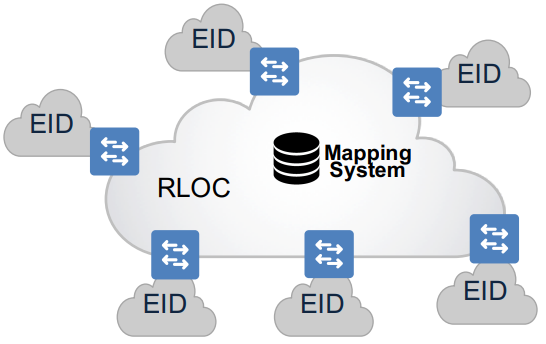
\includegraphics[height=3.5cm]{img/lisp.png}
	\caption{LISP Aufbau}
	\label{fig:LISP Aufbau}
\end{figure}

Dies soll nun durch LISP geändert werden, in dem es die Identität eines Gerätes, auch Endpoint Identifier (EID) genannt, von seinem Aufenthaltsort, auch Routing Locator (RLOC) genannt, in zwei separate Adressräume unterteilt. Das bedeutet, dass die Router in einer LISP-Architektur nur Routing-Informationen von RLOCs speichern müssen. Um Pfadinformationen eines Hosts abzurufen, kann der Router diese beim LISP-Mapping-Server abfragen, was analog wie das DNS-Mapping funktioniert. \\

LISP verwendet für SDA/Fabric eine VXLAN-Kapselung. Um die VXLAN-Kapselung für LISP zu aktivieren, muss auf dem Router der LISP Konfigurationsmodus, den Befehl für die VXLAN-Enkapsulierung verwendet werden. Dieser Befehl muss auf allen LISP-Edge-Geräten im Enterprise-Fabric konfiguriert werden: Ingress Tunnel Router (ITR), Egress Tunnel Router (ETR), Proxy Ingress Tunnel Router (PITR), Proxy Egress Tunnel Router (PETR). Wenn dieser Befehl nicht auf einem der LISP-Edge-Geräte konfiguriert wird, führt dies zu einem Verlust der Kontrolle und des Datenverkehrs.  \cite{rfc-6830}

\begin{table}[H]
	\rowcolors{2}{gray!25}{white}
	\centering
	\begin{tabularx}{\textwidth}{p{6.6cm} | X}
		\rowcolor{gray!50}
		\textbf{LISP Device} & \textbf{Function} \\
		\hline	
		ALT (Alternative Logical Topology) & Collects EID data from Map Servers (MS) and advertise aggregate EID prefix. In a deployment of multiple Map Servers, it keeps all synchronized. \\
		
		ETR (Egress Tunnel Router) and PETR (Proxy ETR) & Connects a LISP capable core network. Registers EID prefices with Map Server (MS). Decapsulates LISP packets, received from LISP core. Responds to Map-request messages with a Map-Reply by giving appropriate EID prefix. Typically, this is a CPE (customer premise equipment) router. PETR works on behalf on non-LISP domain and provides LISP-non-LISP connectivity. \\ 
		
		ITR (Ingress Tunnel Router) and PITR (Proxy Ingress Tunnel Router) & Responsible for forwarding local traffic to external destinations. Resolves RLOC for a given destination by sending Map-request to Map Resolver. Encapsulates (vxlan) traffic with LISP header. Typically, this is a Access Layer Switch. PITR works on behalf on non-LISP domain and provides LISP-non-LISP connectivity. \\
		
		XTR (X Tunnel Router) & When both ITR and ETR functions are handled by one router, it is called XTR. This is typical in practice. \\
		
		MR (Map Resolver) & Responds to Map-requests from ITR. Map-requests will be replied with a Negative Map-Reply or forwarded to appropriate ETR or ALT. \\
		
		MS (Map Server) & Registers EID space upon receiving Map-register messages from ETR. Updates ALT and MR with EID and RLOC data. \\
		
		MSMR (Map Server Map Reloader) & When a device acts as both Map Server and Map Resolver, it is called MSMR. This is typical in practice. \\
		
		EID (Endpoint ID) & Endpoint Identifier. IP addresses hidden from core network routing table. RLOC acts next-hop to reach EID space. \\
		
		RLOC (Routing Locator) & Routing Locator. Exists in global routing tables. Authoritative to reach EID space. \\
		
	\end{tabularx}
	\caption{LISP Elements}
	\label{tab:my-label}
\end{table}

\subsubsection{Campus Fabric und LISP}
Im Einzug mit dem Campus Fabric wurden für bestehende LISP Namenskonzepte neue Begriffsdefinitionen zugewiesen:
\begin{itemize}
	\item "Control-Plane Node" $\approx$ "LISP Map-Server"
	\item "Edge Node" $\approx$ "LISP Tunner Router" (xTR)
	\item "Border Node" $\approx$ "LISP Proxy Tunnel Router" (PxTR)
	\item "Intermediate Node" $\approx$ "Non-LISP IP Forwarder"
\end{itemize}

\subsection{Virtual Extensible LAN (VXLAN)}
VXLAN ist ein Encapsulation-Protokoll, um ein Overlay-Netzwerk auf einer existierenden Layer 3 Infrasturktur laufen zu lassen. VXLAN wurde ursprünglich von Cisco Systems, VMware und Arista Network entwickelt und ist einer der IETF festgelegten Standards (RFC 7348). \cite{rfc-7348} \\
\\
Technisch gesehen erzeugt ein VXLAN logische Layer 2 Netzwerke, die dann in standardmässige Layer 3 Pakete eingepackt werden. VXLAN dient dazu um in sehr grossen Netzwerkumgebung die Probleme zu lösen, die durch beschränkte Anzahl von VLANS betroffen sind. Mit VXLAN sind insgesamt 16’777’215 (24 Bit) Layer-2-Umgebungen möglich, die ihrerseits wieder jeweils 4096 VLANs beinhalten können. 

\subsubsection{VXLAN Encapsulation}
Die Data Plane basiert auf VXLAN, im Gegensatz zur Control Plane, welche auf LISP basiert. Die VXLAN-Kapselung ist IP/UDP-basiert, was bedeutet, dass sie von jedem IP-basierten Netzwerk (Legacy- oder nicht-Cisco-Netzwerk) weitergeleitet werden kann und effektiv den Overlay-Aspekt des SD-Access-Fabric erzeugt. Die VXLAN-Kapselung wird (statt der LISP-Kapselung) aus zwei Hauptgründen verwendet. VXLAN umfasst den Source Layer 2 (Ethernet) -Header (LISP nicht) und bietet auch spezielle Felder für zusätzliche Informationen (wie die ID des virtuellen Netzwerks [VN] und die ID der Gruppe [Segment]). \cite{sda-whitepaper}\\

Diese Technologie bietet mehrere Vorteile für SD-Access, z. B. Unterstützung für virtuelle Layer-2 und Layer-3-Topologien (Overlays) und die Möglichkeit, über jedes IP-basierte Netzwerk mit integrierter Netzwerksegmentierung (VRF/VN) und gruppenbasierter Richtlinie zu arbeiten. \\ 

In SD-Access wurden einige Verbesserungen der ursprünglichen VXLAN-Spezifikationen hinzugefügt, insbesondere die Verwendung von Sicherheitsgruppen-Tags (SGTs). Dieses neue VXLAN-Format ist derzeit ein IETF-Entwurf, der als Gruppenrichtlinienoption (oder VXLAN-GPO) bekannt ist.

\begin{figure}[H]
	\centering
	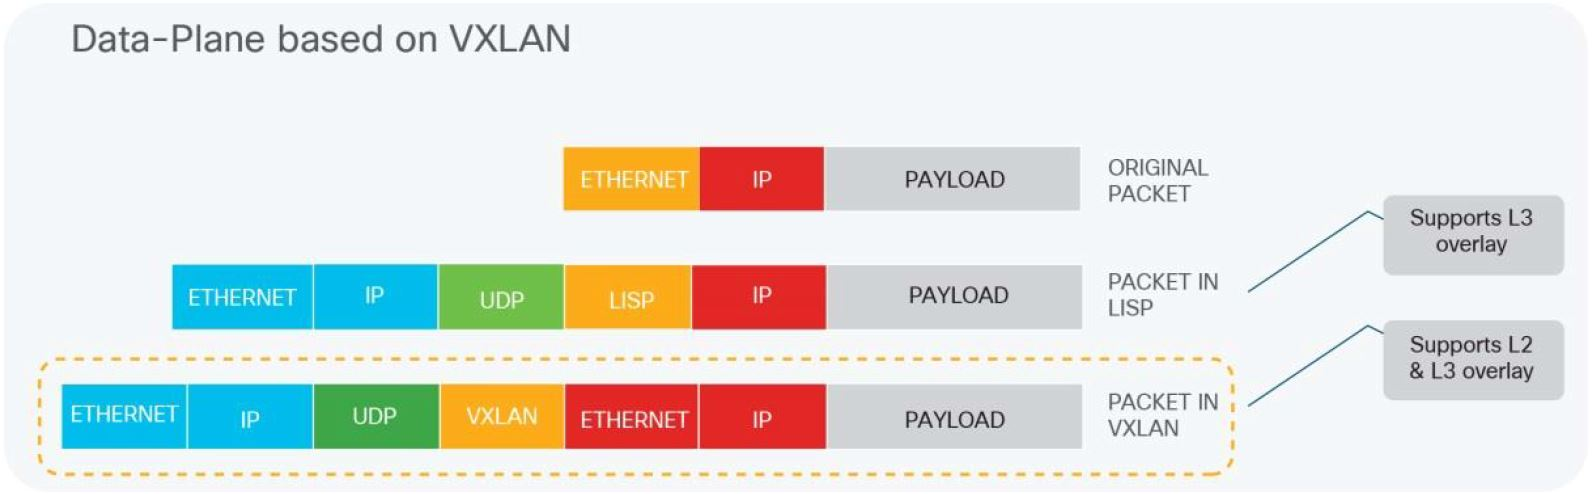
\includegraphics[height=4.5cm]{img/vxlan-encapsulation.jpg}
	\caption{VXLAN Encapsulation}
	\label{fig:VXLAN Encapsulation}
\end{figure}

Die Fabric Data-Plane bietet folgendes:
\begin{itemize}
	\item Underlay Adressanzeige und -zuordnung
	\item Automatischer Tunnelaufbau (Virtuelle Tunnelendpunkte)
	\item Frame-Kapselung zwischen Routing-Locators
\end{itemize}

Unterstützung für das LISP- oder VXLAN-Header-Format
\begin{itemize}
	\item Fast gleich, mit verschiedenen Feldern und Nutzlast
	\item LISP-Header trägt IP-Payload (IP in IP)
	\item VXLAN-Header trägt MAC-Payload (MAC in IP)
\end{itemize}

Ausgelöst durch LISP-Control-Plane-Ereignisse
\begin{itemize}
	\item ARP oder NDP Learning auf L3 Gateways
	\item Map-Reply oder Cache auf Routing Locators
\end{itemize}

\subsection{Slack}
Slack ist ein webbasierter Instant-Messaging-Dienst des US-amerikanischen Unternehmens Slack Technologies zur Kommunikation innerhalb von Arbeitsgruppen. Slack erlaubt, Nachrichten auszutauschen, mit Einzelpersonen oder in einer Gruppe zu chatten sowie gemeinsam Dokumente zu bearbeiten. Andere Online-Dienste wie Dropbox, Google Drive oder GitHub lassen sich in Slack integrieren.

\section{Use Cases} \label{usecases}

\subsection{Use Cases Brief}
\subsubsection{UC01: Definierung von Benutzerprofilen}
Ein Administrator definiert die Profile für Benutzer, Gruppen oder Geräte, sodass diese auf alle nötigen Ressourcen zugreifen können, unberechtigter Zugriff aber verhindert wird.

\subsubsection{UC02: Backup and Restore DNA Center}
Auf Grund eines Problems des DNA Centers muss die Appliance ausgetauscht oder auf einen vorherigen Konfigurationsstand zurückgesetzt werden. Um eine Neukonfiguration des Systems zu verhindern, wird eine zuvor gesicherte Konfiguration wiederhergestellt.

\subsubsection{UC03: Reporting}
Es werden regelmässig Reports über relevante Netzwerkaktivitäten erstellt und den zuständigen Personen via Mail zugestellt.

\subsubsection{UC04: Hardware Ersatz}
Ein Switch muss auf Grund eines Hardwaredefekts oder anderen Gründen ausgetauscht werden.

\subsubsection{UC05: Benutzermobilität}
Ein User ändert seinen Arbeitsplatz, das Gebäude oder den Arbeitsort. Er muss an allen Standorten dieselben Policies erhalten und auf dieselben Ressourcen zugreifen können.

\subsubsection{UC06: Degradation}
Bearbeitung von möglichen Degradations-Szenarien mit entsprechenden Degradations-Tests.

\subsubsection{UC07: Integration von nicht Fabric Komponenten}
Netzintegration von „nicht Campus Fabric Netzkomponenten“ (zum Beispiel traditionelle Access und Distribution Switches).

\subsubsection{UC08:  Migration von bestehendem klassichen Campus}
Migrationskonzept einer bestehenden Campus LAN Lösung zu einer Campus Fabric Lösung mit dem DNA Center.

\subsubsection{UC09: Einsatz von SGT}
Einsatz von SGTs zusammen mit VXLAN (Netzdesign, Design-Rules, Transport innerhalb und ausserhalb der Fabrics, Schnittstelle L2/L3 und Überführung der IP-Konnektivität an ein IP-Backbone wie zum Beispiel MPLS VPN).

\subsubsection{UC10: Infoblox}
Integration Infoblox DNS, DHCP und IPAM (DDI) mit dem DNA Center für die Provisionierung von IP-Adressen für das Management von neuen Netzkomponenten in die Fabric (beispielsweise Access Switches).

\subsection{Use Cases Fully Dressed}
\subsubsection{UC01: Definierung von Benutzer und Geräteprofilen}
\begin{table}[H]
	\rowcolors{2}{gray!25}{white}
	\centering
	\begin{tabularx}{\textwidth}{l | X}
		Primary Actor      & Administrator        \\
		\hline
		Beschreibung       & Ein Administrator definiert die Profile für Benutzer, Gruppen oder Geräte, sodass diese auf alle nötigen Ressourcen zugreifen können, unberechtigter Zugriff aber verhindert wird. \\ 
		\hline
		Stakeholders       &  
		\begin{itemize}	
			\item Administrator
			\item User
		\end{itemize}              \\
		\hline
		Preconditions      & 
		\begin{itemize}	
			\item DNA Center komplett konfiguriert
			\item ISE konfiguriert und mit DNA Center verbunden
		\end{itemize}  \\
		\hline
		Postconditions     & 
		\begin{itemize}	
			\item User kann auf all nötigen Ressourcen zugreifen
			\item Zugriffe auf nicht berechtige Ressourcen werden blockiert
		\end{itemize}  \\
		\hline
		Main Success Story & 
		\begin{enumerate}
			\item Profil wird definiert
			\item Profil wird Usern oder Geräten zugewiesen
			\item Entsprechende Geräte und Benutzer haben Zugriff auf benötigte Ressourcen (und keine zusätzlichen)
		\end{enumerate}
		\\
		\hline
		Alternative Flows  & 
		\begin{itemize}
			\item[1a.] Definitionen fehlen
			\begin{enumerate}
				\item Netzwerksegmente oder Ressourcen definieren
				\item Profil definieren
			\end{enumerate}
			\item[2a.] User oder Geräte fehlen
			\begin{enumerate}
				\item User oder Geräte erfassen
				\item Profil wird Usern oder Geräten zugewiesen
			\end{enumerate}
		\end{itemize}
	\end{tabularx}
	\caption{UC01 Fully Dressed}
	\label{tab:UC01}
\end{table}

\subsubsection{UC02: Backup and Restore DNA Center}
\begin{table}[H]
	\rowcolors{2}{gray!25}{white}
	\centering
	\begin{tabularx}{\textwidth}{l | X}
		Primary Actor   & Netzwerkadministrator        \\
		\hline
		Beschreibung   & Auf Grund eines Problems des DNA Centers muss die Appliance ausgetauscht oder auf einen vorherigen Konfigurationsstand zurückgesetzt werden. Um eine Neukonfiguration des Systems zu verhindern, wird eine zuvor gesicherte Konfiguration wiederhergestellt.  \\ 
		\hline
		Stakeholders       & Alle Netzwerkbenutzer \\ 
		Preconditions      &
		\begin{itemize}	
			\item Ein Backup der DNA Center Konfiguration existiert
		\end{itemize}  \\
		\hline
		Postconditions     & 
		\begin{itemize}	
			\item Appliance läuft mit einer zuvor gesicherten Konfiguration
		\end{itemize}  \\
		\hline
		Main Success Story & 
		\begin{enumerate}
			\item Passendes Backup wählen
			\item Appliance auf den Stand des Backups zurücksetzen
		\end{enumerate}
		\\
		\hline
		Alternative Flows  & -
	\end{tabularx}
	\caption{UC02 Fully Dressed}
	\label{tab:UC02}
\end{table}

\subsubsection{UC03: Reporting}
\begin{table}[H]
	\rowcolors{2}{gray!25}{white}
	\centering
	\begin{tabularx}{\textwidth}{l | X}
		Primary Actor   & Netzwerkadministrator        \\
		\hline
		Beschreibung   & Es werden regelmässig Reports über relevante Netzwerkaktivitäten erstellt und den zuständigen Personen via Mail zugestellt  \\ 
		\hline
		Stakeholders       & 
		\begin{itemize}
			\item Netzwerkadministratoren
			\item Management
		\end{itemize} \\ 
		Preconditions      &
		\begin{itemize}	
			\item Alle nötigen Daten zur Erstellung der Reports stehen im DNA Center zur Verfügung.
		\end{itemize}  \\
		\hline
		Postconditions     & 
		\begin{itemize}	
			\item Definierte Benutzer erhalten regelmässige Reports
		\end{itemize}  \\
		\hline
		Main Success Story & 
		\begin{enumerate}
			\item Relevante Informationen aus dem DNA Center werden erfasst
			\item Informationen werden aufbereitet, Report wird generiert
			\item Report wird per Mail an alle definierten Personen
		\end{enumerate}
		\\
		\hline
		Alternative Flows  & 
		\begin{itemize}
			\item[3a.] Alternativer Messenger
			\begin{enumerate}
				\item Report wird via Slack an alle definierten Personen gesendet
			\end{enumerate}
		\end{itemize}
	\end{tabularx}
	\caption{UC03 Fully Dressed}
	\label{tab:UC03}
\end{table}

\subsubsection{UC04: Hardware Ersatz}
\begin{table}[H]
	\rowcolors{2}{gray!25}{white}
	\centering
	\begin{tabularx}{\textwidth}{l | X}
		Primary Actor   & Netzwerkadministrator        \\
		\hline
		Beschreibung   & Ein Switch muss auf Grund eines Hardwaredefekts oder ähnlichen Gründen ausgetauscht werden.  \\ 
		\hline
		Stakeholders       & 
		\begin{itemize}
			\item Netzwerkadministratoren
			\item User am betroffenen Switch
		\end{itemize} \\ 
		Preconditions      &
		\begin{itemize}	
			\item Ersatzhardware verfügbar
		\end{itemize}  \\
		\hline
		Postconditions     & 
		\begin{itemize}	
			\item Ersatzhardware hat die Funktionalität des auszutauschenden Geräts vollständig übernommen
		\end{itemize}  \\
		\hline
		Main Success Story & 
		\begin{enumerate}
			\item Auszutauschendes Gerät wird entfernt
			\item Neues Gerät wird installiert
			\item Neues Gerät wird verkabelt
			\item Neues Gerät wird im DNA Center erfasst
			\item DNA Center installiert Konfiguration des alten Geräts auf das neue
			\item Neues Gerät übernimmt Funktion des alten Geräts
			\item Altes Gerät im DNA Center entfernen
		\end{enumerate}
		\\
		\hline
		Alternative Flows  & 
		\begin{itemize}
			\item[4a.] Andere Hardware
			\begin{enumerate}
				\item Ersatzhardware ist nicht identisch mit dem alten Gerät
				\item Konfiguration wird im DNA Center angepasst
			\end{enumerate} 
		\end{itemize}
	\end{tabularx}
	\caption{UC04 Fully Dressed}
	\label{tab:UC04}
\end{table}

\subsubsection{UC05: Benutzermobilität}
\begin{table}[H]
	\rowcolors{2}{gray!25}{white}
	\centering
	\begin{tabularx}{\textwidth}{l | X}
		Primary Actor   & Mobiler Benutzer        \\
		\hline
		Beschreibung   & Ein User ändert seinen Arbeitsplatz, das Gebäude oder den Arbeitsort. Er muss an allen Standorten dieselben Policies erhalten und auf dieselben Ressourcen zugreifen können.  \\ 
		\hline
		Stakeholders       & 
		\begin{itemize}
			\item User
		\end{itemize} \\ 
		Preconditions      &
		\begin{itemize}	
			\item User / Gerät erfasst und entsprechende Policies definiert
		\end{itemize}  \\
		\hline
		Postconditions     & 
		\begin{itemize}	
			\item User kann nach einem Standortwechsel alle Ressourcen verwenden, die ihm auch vor dem Wechsel zur Verfügung standen
		\end{itemize}  \\
		\hline
		Main Success Story & 
		\begin{enumerate}
			\item User trennt Verbindung am alten Standort
			\item User verbindet sich am neuen Standort
			\item User authentifiziert sich
			\item Die SDA Lösung gewährt dem User Rechte gemäss Policies
			\item User kann auf dieselben Ressourcen zugreifen wie am alten Standort
		\end{enumerate}
		\\
		\hline
		Alternative Flows  & 
		\begin{itemize}
			\item[4a.]  Während des Standortwechsels wurden die Policies angepasst
			\begin{enumerate}
				\item User erhält Rechte gemäss aktualisierten Policies
			\end{enumerate}
		\end{itemize}
	\end{tabularx}
	\caption{UC05 Fully Dressed}
	\label{tab:UC05}
\end{table}
~
\subsubsection{UC06: Degradation}
\begin{table}[H]
	\rowcolors{2}{gray!25}{white}
	\centering
	\begin{tabularx}{\textwidth}{l | X}
		Primary Actor   & Netzwerkadministrator       \\
		\hline
		Beschreibung   & Es soll aufgezeigt werden, wie sich das System beim Ausfall von verschiedenen Komponenten verhält, wo Single Point of Failures liegen und wie diese allenfalls eliminiert werden können.  \\ 
		\hline
		Stakeholders       & 
		\begin{itemize}
			\item Netzwerkadministrator
			\item Netzwerkbenutzer
		\end{itemize} \\ 
		Preconditions      &
		\begin{itemize}	
			\item Netzwerkinfrastruktur läuft einwandfrei
		\end{itemize}  \\
		\hline
		Postconditions     & 
		\begin{itemize}	
			\item Ausfall/Probleme bei einer oder mehrerer Komponenten
		\end{itemize}  \\
		\hline
		Main Success Story & 
		\begin{enumerate}
			\item Netzwerk funktioniert einwandfrei
			\item Eine oder mehrere Komponenten fallen aus oder weisen sonstige Probleme auf
			\item Netzwerkfunktionalität ist durch den Ausfall nicht beeinträchtigt
			\item Fehler wird behoben, System wieder im Sollzustand
		\end{enumerate}
		\\
		\hline
		Alternative Flows  & 
		\begin{itemize}
			\item[3a.]  Durch den Ausfall kommt es zu einer Störung im Netzwerk
			\begin{enumerate}
				\item Was sind die genauen Auswirkungen? Wer ist betroffen?
				\item Wie kann die Funktionalität wiederhergestellt werden?
				\item Kann die Fehlerursache verhindert werden?
			\end{enumerate}
			\item[3b.]  Es kommt zum kompletten Ausfall des Netzwerks
			\begin{enumerate}
				\item Was sind die genauen Auswirkungen?
				\item Wie kann die Funktionalität wiederhergestellt werden?
				\item Kann die Fehlerursache verhindert werden?
			\end{enumerate}
		\end{itemize}
		\\
		\hline
		Mögliche Szenarien  & 
		\begin{itemize}
			\item Ausfall eines Edge-, Intermediate- oder Border/Controller-Nodes
			\subitem Wenn 1 Node vorhanden ist
			\subitem Wenn 2 Nodes vorhanden sind
			\item Ausfall DNA Center Appliance, ISE, Infoblox, WLC oder einer physischen Netzwerkleitung
		\end{itemize}
	\end{tabularx}
	\caption{UC06 Fully Dressed}
	\label{tab:UC06}
\end{table}

\subsubsection{UC07: Integration von nicht Fabric Komponenten}
\begin{table}[H]
	\rowcolors{2}{gray!25}{white}
	\centering
	\begin{tabularx}{\textwidth}{l | X}
		Primary Actor   & Netzwerkadministrator       \\
		\hline
		Beschreibung   & Die Fabric muss mit Komponenten, die nicht der Fabric angehören kommunizieren können.  \\ 
		\hline
		Stakeholders       & 
		\begin{itemize}
			\item Netzwerkadministrator
			\item Benutzer
		\end{itemize} \\ 
		Preconditions      &
		\begin{itemize}	
			\item Fabric funktioniert
			\item Es sind Komponenten oder Teile des Netzwerks vorhanden, die nicht zu einer Fabric gehören.
		\end{itemize}  \\
		\hline
		Postconditions     & 
		\begin{itemize}	
			\item Kommunikation funktioniert auch über nicht-Fabric Komponenten hinweg
			\item Policies können auch bei Kommunikation über nicht-Fabric Komponenten angewendet werden
		\end{itemize}  \\
		\hline
		Main Success Story & 
		\begin{enumerate}
			\item Ein User kommuniziert mit Ressourcen ausserhalb der Fabric
			\item Kommunikation funktioniert einwandfrei
			\item Policies können wie bei der Kommunikation innerhalb der Fabric angewendet werden
		\end{enumerate}
		\\
		\hline
		Alternative Flows  & 
		\begin{itemize}
			\item[1a.]  Ein User ausserhalb der Fabric will mit Ressourcen innerhalb der Fabric kommunizieren
			\item[2a.] Kommunikation funktioniert einwandfrei
			\item[3a.] Policies können wie bei der Kommunikation innerhalb der Fabric angewendet werden
		\end{itemize}
	\end{tabularx}
	\caption{UC07 Fully Dressed}
	\label{tab:UC07}
\end{table}

\subsubsection{UC08: Migration von bestehenden klassichen Campus}
\begin{table}[H]
	\rowcolors{2}{gray!25}{white}
	\centering
	\begin{tabularx}{\textwidth}{l | X}
		Primary Actor   & Netzwerkadministrator       \\
		\hline
		Beschreibung   & Ein bestehendes Netzwerk nach klassischem Campus Design soll zu einer modernen Fabric migriert werden  \\ 
		\hline
		Stakeholders       & 
		\begin{itemize}
			\item Netzwerkadministrator
			\item Netzwerkbenutzer
		\end{itemize} \\ 
		Preconditions      &
		\begin{itemize}	
			\item Netzwerk nach klassischem Campus Design existiert und funktioniert einwandfrei
			\item DNA Center Appliance inklusive aller Abhängigkeiten ist vorhanden
			\item Netzwerkkomponenten sind fähig in einer Fabric verwendet zu werden
		\end{itemize}  \\
		\hline
		Postconditions     & 
		\begin{itemize}	
			\item Fabric ist erstellt
			\item DNA Center läuft und verwaltet Fabric(s)
			\item Policies, die in der traditionellen Infrastruktur vorhanden waren funktionieren weiterhin
		\end{itemize}  \\
		\hline
		Main Success Story & 
		\begin{enumerate}
			\item Bestehende Infrastruktur wird analysiert und inventarisiert
			\item DNA Center wird aufgesetzt (inkl. aller Abhängigkeiten)
			\item User, Gruppen und Policies werden in DNA Center übernommen
			\item Falls nötig wird das Netzwerkdesign angepasst
			\item Downtime wird geschätzt und organisatorische Massnahmen werden getroffen
			\item Bestehende Netzwerkgeräte werden in die Fabric übernommen
			\item Benutzer können Fabric analog der traditionellen Infrastruktur nutzen
		\end{enumerate}
		\\
		\hline
		Alternative Flows  & -
	\end{tabularx}
	\caption{UC08 Fully Dressed}
	\label{tab:UC08}
\end{table}

\subsubsection{UC09: Einsatz von SGT}
\begin{table}[H]
	\rowcolors{2}{gray!25}{white}
	\centering
	\begin{tabularx}{\textwidth}{l | X}
		Primary Actor   & Administrator       \\
		\hline
		Beschreibung   & Im DNA Center können über das ISE Panel definierte SGT Gruppen hinzugefügt und angepasst werden.  \\ 
		\hline
		Stakeholders       & 
		\begin{itemize}
			\item Administrator
		\end{itemize} \\ 
		Preconditions      & 
		\begin{itemize}	
			\item DNA Center muss mit dem ISE verbunden sein und alle ISE SGT-Gruppen und -Geräte müssen im DNA Center vorhanden sein
		\end{itemize}  \\
		\hline
		Postconditions     & 
		\begin{itemize}	
			\item SGT Gruppen ersichtlich
		\end{itemize}  \\
		\hline
		Main Success Story & 
		\begin{enumerate}
			\item Login auf DNA Center
			\item Unter Systemeinstellungen Cisco ISE Panel auswählen
			\item Unter \textit{Policy $\rightarrow$ Registry $\rightarrow$ Scalable Groups} können neue SGT Gruppen hinzugefügt werden
		\end{enumerate}
		\\
		\hline
		Alternative Flows  & -
	\end{tabularx}
	\caption{UC09 Fully Dressed}
	\label{tab:UC09}
\end{table}

\subsubsection{UC10: Infoblox}
\begin{table}[H]
	\rowcolors{2}{gray!25}{white}
	\centering
	\begin{tabularx}{\textwidth}{l | X}
		Primary Actor   & Administrator       \\
		\hline
		Beschreibung   & Infoblox ist die IP-Adressmanagement-Lösung (IPAM) für das Cisco Digital Network Architecture (DNA) Center. IP-Adresspools werden zwischen DNA Center und Infoblox synchronisiert. Mit dieser Integration kann die Zuweisung von IP-Adressen automatisiert werden, was eine richtlinienbasierte Bereitstellung in einem einzigen Vorgang ermöglicht und so die Betriebseffizienz verbessert.  \\ 
		\hline
		Stakeholders       & 
		\begin{itemize}
			\item Administrator
		\end{itemize} \\ 
		Preconditions      &
		\begin{itemize}	
			\item Infoblox Server ist eingerichtet
		\end{itemize}  \\
		\hline
		Postconditions     & 
		\begin{itemize}	
			\item Unter \textit{Design $\rightarrow$ Network Settings $\rightarrow$ IP Address Pools} sind nun die IP-Adressen ersichtlich.
			\item Anpassungen an Addresspool werden zwischen DNA Center und Infoblox synchronisiert
			\item Infoblox verwendet die im DNA Center erstellten Infos für weitere Dienste wie DNS oder DHCP
		\end{itemize}  \\
		\hline
		Main Success Story & 
		\begin{enumerate}
			\item Login auf DNA Center
			\item Unter \textit{Settings $\rightarrow$ IP Adress Manager} kann ein Infoblox Server hinterlegt werden.
			\item Unter \textit{Design $\rightarrow$ Network Settings $\rightarrow$ IP Address Pools} können nun die IP-Adressen angezeigt werden
		\end{enumerate}
		\\
		\hline
		Alternative Flows  & 
		\begin{itemize}
			\item[1a.] Direkt nach der Installation des DNA Centers, Infoblox Server bei erstem Konfigurations-Wizard hinzufügen
			\begin{enumerate}
				\item Login auf DNA Center
				\item IPAM angeben (Server Name, Server URL, Username, Password, Provider)
			\end{enumerate}
			\item[1b.] Schritt in erstem Konfigurations-Wizard überspringen und Infoblox mit nachfolgenden Schritten hinzufügen.
		\end{itemize}
	\end{tabularx}
	\caption{UC10 Fully Dressed}
	\label{tab:UC10}
\end{table}



\begin{landscape}
\section {Testprotokolle}

\testpttb{UC01-1: Anlegen von Benutzern}{}{
\testptrow{1}{Login in ISE}{Eingelogged in ISE}{Eingelogged in ISE}{OK}
\testptrow{2}{Benutzer anlegen via \textit{Work Centers $\rightarrow$ Network Access $\rightarrow$ Identities $\rightarrow$ Network Access Users}}{User ist erstellt}{User ist erstellt}{OK}
\testptrow{2}{Benutzer einer Gruppe zuweisen via \textit{Work Centers $\rightarrow$ Network Access $\rightarrow$ Identities $\rightarrow$ Network Access Users}}{User ist in Gruppe}{User ist in Gruppe}{OK}
}

Die Benutzer sind nun angelegt, ein Login ist aber noch nicht möglich, da noch keine Authentication Policy für diese erstellt wurde. Dies wird daher im nächsten Schritt erledigt.

\testpttb{UC01-2: Anlegen von Authentication Policies}{}{
	\testptrow{1}{Login in ISE}{Eingelogged in ISE}{Eingelogged in ISE}{OK}
	\testptrow{2}{Authentication Policy anlegen via \textit{Work Centers $\rightarrow$ Network Access $\rightarrow$ Policy Sets $\rightarrow$ Default} für 802.1x Wired}{Policy ist erstellt}{Policy ist erstellt}{OK}
	\testptrow{3}{User logged sich ein}{User ist eingelogged}{User ist eingelogged}{OK}
}

Nun kann sich der Benutzer einloggen, wird aber noch nicht einer Scalable Group zugewiesen. Somit hat er keine für ihn gültige Policy und somit keine Zugriffe im Netzwerk. Damit der Benutzer die korrekten Policies erhält, muss eine Authorization Policy erstellt werden.

\testpttb{UC01-3: Anlegen von Authorization Policies}{}{
	\testptrow{1}{Login in ISE}{Eingelogged in ISE}{Eingelogged in ISE}{OK}
	\testptrow{2}{Authorization Policy anlegen via \textit{Work Centers $\rightarrow$ Network Access $\rightarrow$ Policy Sets $\rightarrow$ Default} für 802.1x Wired und Gruppe des Users}{Authorization Policy ist erstellt}{Authorization Policy ist erstellt}{OK}
	\testptrow{3}{User wird beim Login der korrekten SG zugewiesen}{User ist der korrekten Gruppe zugewiesen}{User ist der korrekten Gruppe zugewiesen}{OK}
}

\testpttb{UC01-4: Einrichten einer Policy}{}{
	\testptrow{1}{Login auf DNA Center}{DNA Center Dashboard wird angezeigt}{DNA Center Dashboard wird angezeigt}{OK}
	\testptrow{2}{Policy einrichten unter \textit{Policy $\rightarrow$ Policy Administration $\rightarrow$ Group Based Access Control}}{Policy wird angelegt}{Policy wird angelegt}{OK}
	\testptrow{3}{DNA Center synchronisiert Policy mit dem ISE}{Policy ist auf ISE}{Policy ist auf ISE}{OK}
	\testptrow{4}{ISE pushed Policy auf Border und Edge Nodes}{Policy ist auf Nodes vorhanden}{Policy ist auf Nodes vorhanden}{OK}
	\testptrow{5}{Die Nodes enforcen die Policy für die korrekten Clients}{Policy wird enforced}{Policy wird enforced}{OK}
}

Die Policy ist nun auf allen nötigen Geräten deployed und wird von diesen enforced. Die Clients dürfen also nur auf die Ressourcen zugreifen, die gemäss der definierten Policy erlaubt sind.
\pagebreak

\testpttb{UC02-1 Backup DNA Center}{Sämtliche Konfigurationen des DNA Centers sollen gebackuped werden, sodass diese im Notfall wiederhergestellt werden können.}{
	\testptrow{1}{Login auf DNA Center}{DNA Center Dashboard wird angezeigt}{DNA Center Dashboard erscheint}{OK}
	\testptrow{2}{Zu den Backup Einstellungen navigieren \textit{Settings $\rightarrow$ System Settings $\rightarrow$ Backup and Restore} }{Backup Einstellungen anzeigen}{Backup Einstellungen erscheinen}{OK}
	\testptrow{3a}{Backup Server hinzufügen via \textit{Add} $\rightarrow$ SSH IP Address: 217.26.58.9, SSH Port: 22, Server Path: /home/dnacenter/backup, Username: dnacenter, Password: xxx, Encryption Passphrase: xxx. Mittels Apply die Eingaben bestätigen.}{Eingaben werden angenommen.}{Eingaben werden meist nicht angenommen und führen zu Absturz des DNA Centers}{NOT OK}
	\testptrow{3b}{Backup Server hinzufügen via \textit{Add} $\rightarrow$ SSH IP Address: 217.26.58.9, SSH Port: 22, Server Path: /home/dnacenter/backup, Username: dnacenter, Password: xxx, Encryption Passphrase: xxx. Mittels Apply die Eingaben bestätigen.}{Eingaben werden angenommen.}{Eingaben werden angenommen.}{OK}
	\testptrow{4b}{Regelmässiges Backup einrichten via \textit{Schedule $\rightarrow$ Add} Schedule Later, Weekday: Wednesday, Time: 10:30 AM. Mittels Schedule die Eingaben bestätigen.}{Eingaben werden angenommen.}{Eingaben werden angenommen.}{OK}
	\testptrow{5b}{Backup wird regelmässig zum definierten Zeitpunkt ausgeführt.}{Backup wird zum definierten Zeitpunkt ausgeführt}{Backup wird nicht ausgeführt}{NOT OK}
}

\testpttb{UC02-2 Restore DNA Center}{Sämtliche Konfigurationen des DNA Centers sollen aus einem zuvor erstellten Backup wiederhergestellt werden.}{
	\testptrow{1}{Login auf DNA Center}{DNA Center Dashboard wird angezeigt}{DNA Center Dashboard erscheint}{OK}
	\testptrow{2}{Zu den Backup Einstellungen navigieren \textit{Settings $\rightarrow$ System Settings $\rightarrow$ Backup and Restore} }{Zuvor erstellte Backups werden angezeigt}{Backups werden angezeigt}{OK}
	\testptrow{3}{Restore erstellen via \textit{Restore} neben dem gewünschten Backup}{DNA Center wird auf den Stand vom gewählten Backup zurückgesetzt}{DNA Center wurde auf den gewünschten Stand zurückgesetzt}{OK}
}

\subsubsection{Zusammenfassung UC02}
Es kann ein Backup erstellt werden und auch ein Restore eines zuvor erstellten Backups ist möglich. Leider ist das Erfassen, Bearbeiten und Löschen eines Backupservers enorm unzuverlässig und hat mehrfach zu kompletten Abstürzen des DNA Centers geführt. \\
Zudem funktioniert der Backup Schedule nicht. Backups werden nicht automatisch ausgeführt, sind also nur manuell möglich. Auch ein Restore einzelner Komponenten des DNA Centers ist nicht vorgesehen und es gibt kein komplettes Backup des DNA Centers. Einzelne Teile wie z.Bsp. Assurance werden nicht gebackuped. \\
Da die Backup Funktionalität des DNA Centers sehr eingeschränkt ist und nur unzuverlässig funktioniert, wird der Use Case "Backup und Restore" nicht vollständig erfüllt.
\pagebreak

\testpttb{UC03 Reporting}{Mit Hilfe der DNA Center API können regelmässige Reports über den Zustand der Netzwerkumgebung per E-Mail oder Slack versendet werden. Damit dieser Use Case ausgeführt werden kann, muss ein Mailserver und ein Benutzer zur Verfügung stehen, der E-Mails versenden kann. Des weiteren ist ein System benötigt, welches das Script ausführt. Auf diesem muss python installiert sein.}{
	\testptrow{1}{Reporting Script aus GIT Repository auschecken (auf dem System, das die Reports versenden soll)}{Code ist ausgecheckt}{Code ist ausgecheckt}{OK}
	\testptrow{2}{config.py mit Texteditor öffnen und anpassen}{Reporting Config ist komplett}{Reporting Config ist komplett}{OK}
	\testptrow{3}{Cronjob einrichten, der das Script in regelmässigen Abständen ausführt}{Script wird regelmässig ausgeführt}{Script wird regelmässig ausgeführt}{OK}
	\testptrow{4a}{Cronjob wird ausgeführt und versendet Report per E-Mail}{Report wird per E-Mail versendet.}{Report wird per E-Mail versendet}{OK}
	\testptrow{4b}{Cronjob wird ausgeführt und versendet Report per Slack}{Report wird per Slack versendet.}{Nicht implementiert}{NOT OK}
}

\subsubsection{Zusammenfassung UC03}
Mit dieser Lösung ist ein sehr rudimentäres Reporting implementiert worden. Es wird lediglich eine Liste aller Netzwerkgeräte, sowie eine Liste aller Hosts mit den wichtigsten Informationen und dem Zustand der Geräte ausgegeben. Wünschenswert wären natürlich wesentlich mehr Informationen, insbesondere aus dem Bereich Assurance. Leider unterstützt die API des aktuellen Release 1.1.6 diese Funktionien nicht. Im Release 1.2 ist einiges mehr vorhanden, aber nach wie vor als Early Field Trial (EFT) gekennzeichnet. 
Eine sinnvolle Reporting Funktion ist daher mit den aktuell verfügbaren APIs des DNA Centers nicht realisierbar.
\pagebreak

\subsection{UC04: Hardware Ersatz}
Wenn ein Device in der Fabric ausfällt, ist folgendermassen vorzugehen, um dieses auszutauschen und den alten Stand der Fabric wiederherzustellen.\\
\begin{itemize}
	\item Altes Gerät durch neues ersetzen
	\item Neues Gerät identisch verkabeln
	\item Das Gerät mittels LAN Automation wieder in Betrieb nehmen
	\item Device Provisioning ausführen
	\item Device der ursprünglichen Fabric hinzufügen
	\item Device Provisioning erneut ausführen
	\subitem Sofern der Gerättyp zwischen altem und neuen Device identisch ist, sollte die Access Portkonfiguration übernommen werden
	\subitem Sind es unterschiedliche Gerätetypen müssen die Access Ports manuell konfiguriert werden
	\item Der neue Switch sollte nun die komplette Funktion des alten übernommen haben\\
\end{itemize}

Die obigen Informationen sind nur theoretisch und konnten in der Testumgebung nicht getestet werden.
\pagebreak


\testpttb{UC05 Benutzermobilität}{Ein User ändert seinen Arbeitsplatz, das Gebäude oder den Arbeitsort. Er muss an allen Standorten dieselben Policies erhalten und auf dieselben Ressourcen zugreifen können.}{
	\testptrow{1}{User ist in Gebäude 1 mit dem Netzwerk verbunden}{User ist mit dem Netzwerk verbunden}{User ist mit dem Netzwerk verbunden}{OK}
	\testptrow{2}{User authentifiziert sich und erhält die korrekten Policies}{User erreicht nur die Ressourcen, die per Policy erlaubt sind}{User erreicht nur die Ressourcen, die per Policy erlaubt sind}{OK}
	\testptrow{3}{User trennt Verbindung in Gebäude 1}{Verbindung ist getrennt}{Verbindung ist getrennt}{OK}
	\testptrow{4}{User verbindet sich im Gebäude 2}{User ist mit dem Netzwerk verbunden}{User ist mit dem Netzwerk verbunden}{OK}
	\testptrow{5}{User authentifiziert sich}{User ist authentifiziert}{User ist authentifiziert}{OK}
	\testptrow{6}{User erhält die korrekten Policies}{User erreicht dieselben Ressourcen wie zuvor in Gebäude 1}{User erreicht dieselben Ressourcen wie zuvor n Gebäude 1}{OK}
}

\subsubsection{Zusammenfassung UC05}
Benutzermobilität funktioniert in einer vom DNA Center verwalteten sehr gut. In unseren Tests wurden sogar bestehende Sessions vom alten an den neuen Standort übernommen. 
\pagebreak
\subsection{UC06: Degradation}
In diesem Use Case wird beschrieben, wie sich das Netzwerk verhält, wenn einzelne Komponenten ausfallen. In untenstehender Tabelle ist zu sehen, was für einen Impact der Ausfall der einzelnen Komponenten hat. Die Informationen sind allerdings nur theoretisch und konnten in der Lab Umbegung nicht getestet werden.
\\

\rowcolors{2}{gray!25}{white}
\begin{longtable}{| m{2.5cm} | m{21.5cm} |}
		\hline
		\textbf{Ausfall Gerät}  & \textbf{Impact}        \\
		\hline
		Edge Node  & Alle Clients an diesem Device verlieren die Konnektivität.  \\ 
		\hline
		Intermediate Node & Kein Impact solange alle Edge Devices noch einen Pfad zum Border und somit zu den anderen Edge Nodes haben \\ 
		\hline
		Border Node & Kein Impact, solange ein weiterer Border verhanden ist. Falls nicht, verliert die Fabric die Kommunikation zu Geräten ausserhalb der Fabric \\
		\hline
		Control Plane & Kein Impact, solange eine weitere Control Plane vorhanden ist. Falls nicht, können die Edge Nodes den RLOC von Clients nicht mehr ermitteln und müssen auf den eigenen Cache zurückgreifen. Die Kommunikation innerhalb und ausserhalb der Fabric ist also eingeschränkt. Sobald die TTL der Cache Einträge abgelaufen ist, ist nur noch Kommunikation zwischen Clients am gleichen Edge Node möglich. \\
		\hline
		DNA Center & Ein Ausfall des DNA Centers hat keinen direkten Einfluss auf das Netzwerk. Es können allerdings keine Anpassungen mehr gemacht werden, die Assurance Daten stehen nicht zur Verfügung und werden nicht mehr erfasst. \\
		\hline
		ISE & Fällt der ISE aus und es ist kein weiterer ISE vorhanden, können sich Benutzer nicht mehr am Netzwerk authentifizieren und die Policies sind nicht mehr verfügbar. Das heisst, der Netzwerkbetrieb ist stark eingeschränkt oder gar komplett unterbrochen. Es gibt daher die Möglichkeit, ein "Notfall VLAN" zu definieren, über welches die Clients in diesem Fall weiterhin kommunizieren könnten. \\
		\hline
		Infoblox & Fällt Infoblox aus, können keine neuen IP Pools angelegt werden. Des Weiteren funktioniert DNS nicht mehr, sofern Infoblox der einzige DNS Server war. Dasselbe gilt auch für DHCP. \\
		\hline
		Kabelunter- bruch & Ein Kabelunterbruch zwischen zwei Netzwerkkomponenten in der Fabric hat keinen Impact auf den Betrieb, sofern alle Edge Nodes über Pfade zu den anderen Edge Nodes und dem Border verfügen.\\
		\hline
	\caption{UC06: Testprotokoll Degradation}
	\label{tab:UC06_Testprotokoll}
\end{longtable}
\pagebreak

\subsection{UC07: Integration von nicht Fabric Komponenten}
Der Einsatz von nicht Fabric Komponenten ist im aktuellen Release nicht unterstützt. Es ist aber vorgesehen, dass im Release 1.2 die "SD Access Extension for IoT" eingeführt wird, mit der die Fabric mit Hilfe von Geräten wie zum Beispiel dem C3650CX erweitert werden kann.
\pagebreak

\subsection{UC08: Migration von bestehendem klassischen Campus}
Es gibt derzeit keinen definierten Migrationspfad von einem klassischen Campus Netzwerk. Die Empfehlung von Cisco ist allerdings wie folgt:
\begin{itemize}
	\item Parallel zu bestehendem Netzwerk einen Border Node aufsetzen
	\item Mit Hilfe der LAN Automation einen Intermediate Node in Betrieb nehmen
	\item Mit Hilfe der LAN Automation einen ersten Edge Node in Betrieb nehmen
	\item Fabric erstellen
	\item User, Policies usw. definieren
	\subitem Schrittweise Clients migrieren
	\item Schrittweise weitere Nodes (Border, Intermediate, Edge) hinzufügen
\end{itemize}

Werden Devices aus einem klassischen Netz in die Fabric übernommen, sollten die Konfiguration zuerst gelöscht werden. 
Dieses Vorgehen wird von Cisco so empfohlen, konnte aber in unserer Testumgebung nicht getestet werden, da ein Parallelbetrieb einer klassischen Umgebung und der Fabric zu aufwändig gewesen wäre.
\pagebreak

\testpttb{UC09: Einsatz von SGT}{Erstellen einer neuen Scalable Group.}{
	\testptrow{1}{Login auf DNA Center}{DNA Center Dashboard wird angezeigt}{DNA Center Dashbaord erscheint}{OK}
	\testptrow{2}{Zu den Einstellungen navigieren \textit{Policy  $\rightarrow$ Registry $\rightarrow$ Scalable Groups }}{Liste der \textit{Scalable Groups} wird angezeigt, inklusive der \textit{Add Group} Schaltfläche.}{Liste der \textit{Scalable Groups} wird angezeigt, inklusive der \textit{Add Group} Schaltfläche.}{OK}
	\testptrow{2}{Hinzufügen einer neuer Gruppe mithilfe der Schaltfläche \textit{Add Group}}{Neuer Dialog erscheint zum Anlegen einer \textit{Scalable Group.}}{Weiterleitung zum Cisco ISE zur Ansicht \textit{Components $\rightarrow$ Security Groups.} (Eventuell muss man sich zuvor beim ISE zusätzlich einloggen.) Dort muss \textit{Add} ausgewählt werden. Es erscheint ein Dialog zum Hinzufügen einer \textit{Security Group.}}{NOT OK}
	\testptrow{3}{Neue Gruppe anlegen mit einem Namen}{Im Dialog kann ein neuer Name für die \textit{Scalable Group} eingegeben werden. Der Dialog wird mit \textit{Speichern} geschlossen. }{Ein neuer Name, ein Symbol und eine Beschreibung kann hinterlegt werden. Zusätzlich muss \textit{Propagate to ACI} angewählt werden. Der Dialog wird mit \textit{Anlegen} geschlossen}{OK}
	\testptrow{4}{Die Scalable Group ist erstellt.}{In der Liste der Scalable Groups wird die neu erstellte Gruppe angezeigt.}{Da man immernoch in der ISE Ansicht ist, muss zuerst zum alten Tab des DNA Centers gewechselt werden. Anschliessend muss die Seite neu geladen werden. Die neue erstellte Gruppe wird angezeigt.}{OK}
}

\subsubsection{Zusammenfassung UC09: Einstaz von SGT}
Noch nicht alle Funktionen können komplett im DNA Center erledigt werden. Ein Teil der Funktionen erfolgt weiterhin über die GUI der anderen Komponenten. 

\pagebreak

\testpttb{UC10-1: Infoblox verknüpfen}{Durch die Integration des Infoblox DDI im DNA Center soll das IP-Adressen Management für neue Netzwerkkomponenten vereinfacht werden.}{
	\testptrow{1}{Login auf DNA Center}{DNA Center Dashboard wird angezeigt}{DNA Center Dashboard erscheint}{OK}
	\testptrow{2}{Zu IP Adress Manager Einstellungen navigieren über \textit{Settings $\rightarrow$ System Settings $\rightarrow$ Settings $\rightarrow$ IP Adress Manager} }{IP Adress Manager Einstellungen anzeigen}{IP Adress Manager Einstellungen erscheinen}{OK}
	\testptrow{3}{Infoblox Informationen hinterlegen $\rightarrow$ Server Name: Infoblox, Server Url: https://10.22.0.21, Username: admin, Password: xxx, Provider: INFOBLOX). Mittels Apply die Eingaben bestätigen.}{Eingaben werden angenommen.}{Eingaben wurden angenommen und Verbindung zu Infoblox Server erfolgreich hergestellt.}{OK}
}

\testpttb{UC10-2: IP Adress Pool erstellen}{IP Adress Pools auf dem Infoblox erstellen und mit DNA Center synchronisieren}{
	\testptrow{1}{IP Adress Pools anzeigen über \textit{Design $\rightarrow$ Network Settings $\rightarrow$ IP Adress Pools}.}{IP Adress Pools sollten angezeigt werden.}{Es werden vorhandene IP Adress Pools angezeigt.}{OK}
	\testptrow{2}{Mit einem Klick auf \textit{Add IP Pool} kann ein neuer IP Pool hinzugefügt werden. Hierfür werden folgende Angaben benötigt: IP Pool Name, CIDR Prefix, IP Subnetz, Gateway IP Adresse, DHCP Server (optional), DNS Server (optional)}{Fenster um IP Adress Pool hinzuzufügen erscheint}{Fenster um IP Adress Pool hinzuzufügen ist erschienen}{OK}
	\testptrow{3}{Mit einem Klick auf Save wird der IP Adress Pool hinzugefügt und mit dem Infoblox Server synchronisiert}{Übersicht über vorhandene IP Adress Pools wird angezeigt}{Übersicht über vorhandene IP Adress Pools wird angezeigt mit vorher hinzugefügtem IP Adress Pool}{OK}
}

\subsubsection{Zusammenfassung UC10}
Der Infoblox konnte im DNA Center relativ einfach hinterlegt werden. Das erstellen eines IP Adress Pools auf dem DNA Center funktioniert gut und wird auch schnell mit dem Infoblox synchronisiert. Wird jedoch ein IP Adress Pool auf dem Infoblox erstellt, so ist es eher mühsam diesen neuen IP Adress Pool auf dem DNA Center anzuzeigen. Diese Synchronisation erfolgt nicht sauber. Es ist auf dem DNA Center zwar eine Import Funktion vorhanden, welche die IP Adress Pools vom Infoblox importieren sollte, aber nur mässig gut funktioniert. Jedes Netz welches importiert werden soll, muss einzeln erstellt und genaustens angegeben werden. Aus diesem Grunde sollte generell alles was im DNA Center erstellt werden kann, auf diesem erstellt werden und nicht manuell auf dem Infoblox.

\pagebreak


\end{landscape}
\section{Umsetzung}

\begin{itemize}
	\item Ausgewählte Implementierungsdetails (Bsp. Algorithmen, Datenstrukturen, Libraries, Architectural Hot Spots)Dokumentation Architektur und Design (i.d.R. plattformneutral bzw. technologieübergreifend, z.B. in Form von UML-Diagrammen und Erläuterungen dazu)
	\item Dokumentation, welche Experimente/Tests durchgeführt wurden und welche Lösungsoptionen aufgrund der Ergebnisse dieser Experimente/Tests verworfen wurden.
\end{itemize}

\subsection{Labor Netzwerk Architektur}
Mit der zur Verfügung gestellten Hardware ist die folgende Netzwerk Architektur entstanden.

Folgende zentrale Überlegungen sind eingeflossen:

\begin{itemize}
	\item Campus Netzwerk mit mehreren Gebäuden, um das Wandern von Geräten zu simulieren.
	\item Mischung der zur Verfügung stehenden Switches (Catalyst 9300 \& 3850) in der Fabric Edge Nodes, um Verhalten zu vergleichen.
	\item Management Netzwerk ist inbound. Kabelführung zu jedem Switch ist meistens von den Gegebenheiten in typsichen Gebäuden nicht möglich.
\end{itemize}


\begin{figure}[H]
	\centering
	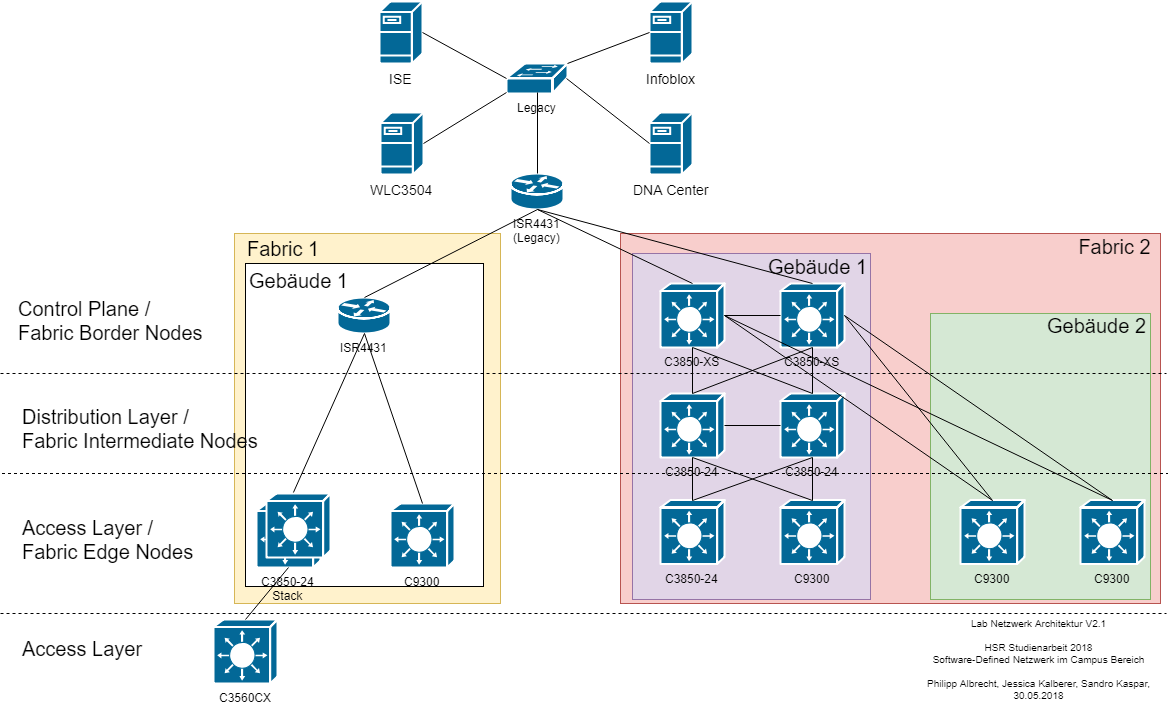
\includegraphics[height=10cm]{img/LabNetworkArchitecture.png}
	\caption{SDN Netzwerk Architektur}
	\label{fig:LabNetworkArchitecture}
\end{figure}

\subsection{Netzwerkarchitekturen Vergleich}
Hauptunterschiede zwischen der klassischen Netzwerkarchitektur und der "Modernen" Software-Defined Access Architektur. 

\begin{itemize}
	\item Bis zur Fabric Edge Nodes (Vergleichbar mit dem Access Layer) unterliegt ein Layer 3 Netzwerk. 
	\item Kein Einsatz von STP oder VSS auf Distribution Layer notwendig, da das Underlay Netzwerk rein Layer 3 ist und Routing Protokolle (OSPF) zum Einsatz kommen.
	\item Der Distribution Layer nimmt neu als Fabric Intermediate Nodes nur noch die Funktion als Layer 3 Brücke bzw. VXLAN transporteuer ein, anstatt die Grenze zwischen Layer 3 und Layer 2 zu sein. Die Fabric Intermediate Nodes sind optional. 
	\item Während beim klassischen Design die logische Netzwerkarchitektur direkt Abhängig ist von der physikalischen Architektur, wird bei SDN die phykalische Netzwerkarchitektur von der logischen Architektur getrennt. Man spricht dann von der Physical Fabric Topology bzw. Underlay und den entsprechenden Layer 2 bzw. Layer 3 Overlay Network. 
\end{itemize}

\begin{figure}[H]
	\centering
	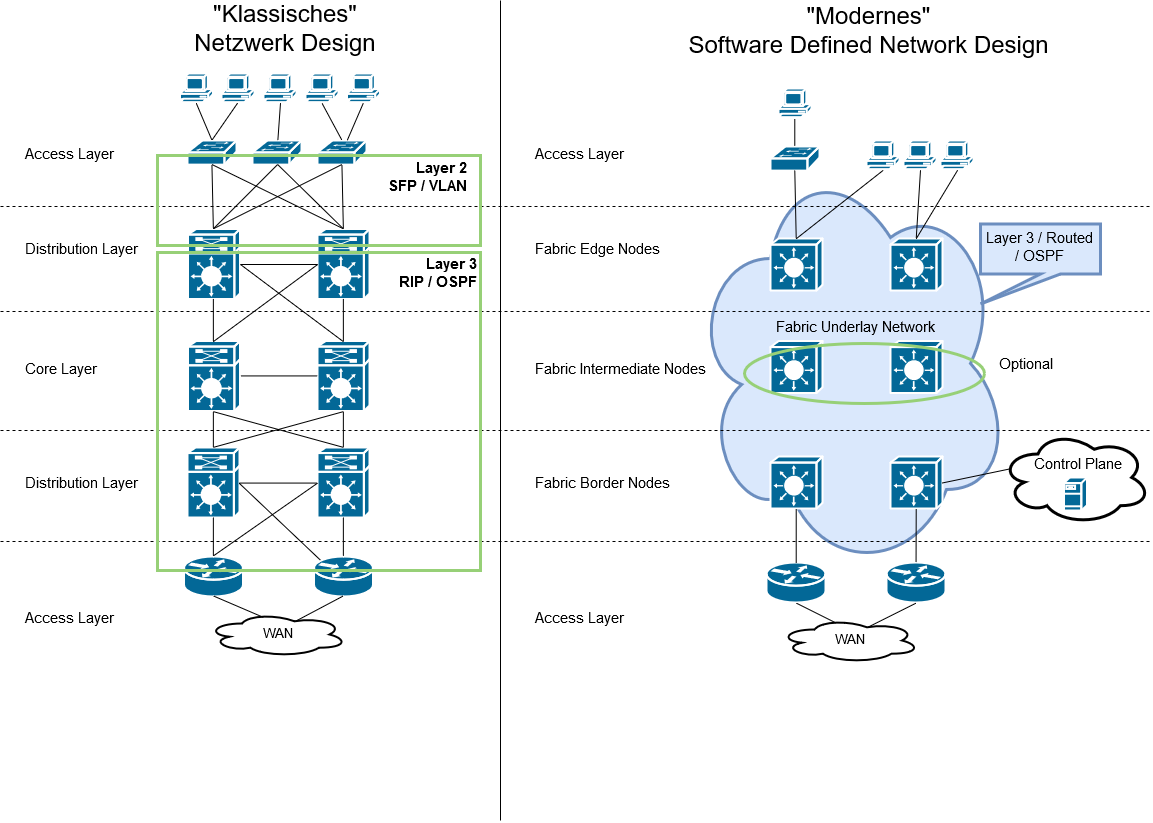
\includegraphics[height=12cm]{img/LabNetworkArchitecture_Vergleich.png}
	\caption{Netzwerk Architektur Vergleich}
	\label{fig:LabNetworkArchitectureVergleich}
\end{figure}

\pagebreak
\subsection{Verkabelungsplan}
\begin{longtable}{| l | l | l | l |}
		\hline
		\multicolumn{4}{| c| }{Verkabelung} \\
		\hline
		\multicolumn{2}{| c |}{Seite A} & \multicolumn{2}{ c |}{Seite B} \\
		\hline
		isr4431-1.access & GE0/0/0 & WAN & -\\
		\hline
		isr4431-1.access & GE0/0/1 & isr4431-2.access & GE0/0/1 \\
		\hline
		isr4431-1.access & GE0/0/2 & c9300-1.dist & GE1/0/1 \\
		\hline
		isr4431-2.access & GE0/0/0 & WAN & - \\
		\hline
		isr4431-2.access & GE0/0/1 & isr4431-1.access & GE0/0/1 \\
		\hline		
		c9300-1.dist & GE1/0/2 & c9300-2.dist & GE1/0/2  \\
		\hline
		c9300-1.dist & GE1/0/3 & isr4431-1.core & GE0/0/0 \\
		\hline
		c9300-2.dist & GE1/0/3 & isr4431-2.core & GE0/0/0 \\
		\hline
		c9300-2.dist & GE1/0/4 & HSR Lab & - \\
		\hline
		isr4431-1.core & GE0/0/1 & isr4431-2.core & GE0/0/1 \\
		\hline
		isr4431-1.core & GE0/0/2 & c3850.g1.dist & GE1/0/1 \\
		\hline
		isr4431-1.core & GE0/0/3 & c3850.g2.access & GE1/0/1 \\
		\hline
		isr4431-1.core & GE0/1/0 & c9300.g3.access & GE1/0/1 \\
		\hline
		isr4431-2.core & GE0/0/2 & c3850.g1.dist & GE2/0/1 \\
		\hline
		isr4431-2.core & GE0/0/3 & c3850.g2.access & GE1/0/2 \\
		\hline
		isr4431-2.core & GE0/1/0 & c9300.g3.access & GE1/0/2 \\
		\hline
		c3850.g1.dist & GE1/0/2 & c3850.g1.access & GE1/0/1 \\
		\hline
		c3850.g1.dist & GE2/0/2 & c9300.g1.access & GE1/0/1 \\
		\hline
		c3850.g1.access & GE1/0/3 & c3650.g1.access & GE0/1 \\
		\hline
\end{longtable}
\section{Vorgehen}
Nachfolgend haben wir das Vorgehen von unserem ersten Versuch in einer Grafik übersichtlich dargestellt. Die Blitze deuten dabei auf ein Hindernis bei welchem mehr Aufwand benötigt wurde hin und das rote X als einen fehlgeschlagenen Versuch, welcher abgebrochen werden musste.
\begin{figure}[H]
	\centering
	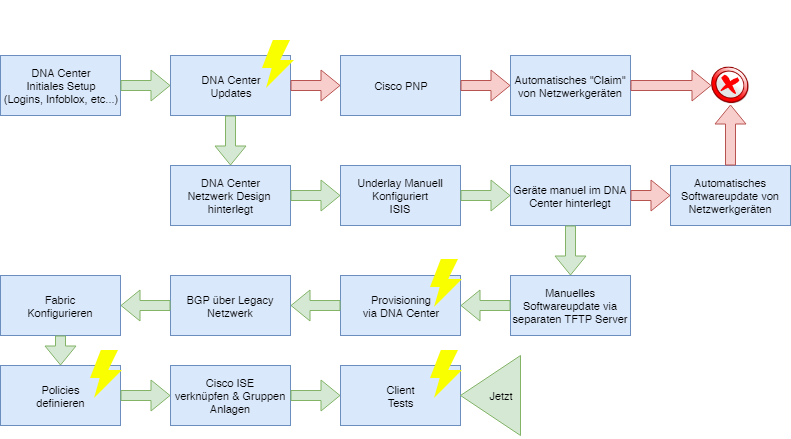
\includegraphics[height=9cm]{img/vorgehen.png}
	\caption{Übersicht Vorgehen}
	\label{fig:vorgehen}
\end{figure} 

\subsection{DNA Center Initiales Setup}

\subsubsection{Installation}
\label{DNACenterSetup_Installation}
Die Installation des DNA Centers erfolgt direkt an der Konsole oder über die Cisco IMC. Dabei wird der maglev-config-wizard ausgeführt. Dieser Befehl kann zu einem späteren Zeitpunkt erneut ausgeführt werden, wenn die Konfiguration angepasst werden muss.

Wie in Kapitel 2\cite{cisco-dna-installation-guide} beschrieben werden folgende Angaben benötigt:
\begin{itemize}
	\item Host IP Adresse
	\item Netmask
	\item Default Gateway IP adress
	\item DNS Servers
	\item Static Routes
	\item HTTPS Proxy
	\item Maglev Master Node IP
	\item Username, Passwort und Linux Passwort
	\item Administration Passphrase für das Web-Interface
	\item NTP Server
	\item Service Subnets
\end{itemize}

Im ersten Schritt \ref{fig:dna-center-install-step-1} wird gewählt, ob ein neuer Cluster erstellt werden soll oder einem beigetreten werden soll. Bei der Testumgebung dieser Arbeit war nur eine Appliance verfügbar, weshalb schliesslich "Start a DNA-C Cluster" ausgewählt wurde. 

\begin{figure}[H]
	\centering
	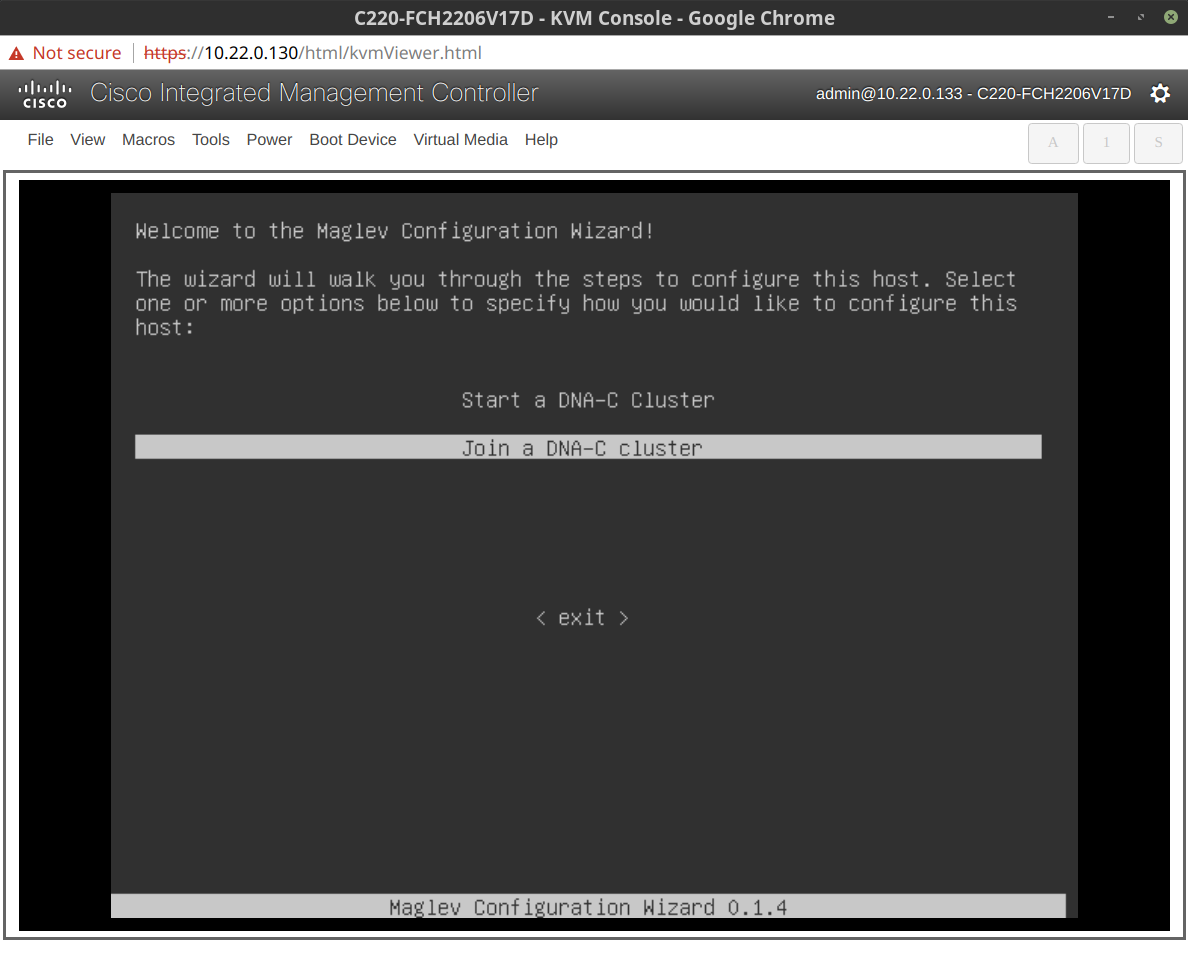
\includegraphics[height=9cm]{img/sc_001.png}
	\caption{DNA Center Configuration Wizard - Start}
	\label{fig:dna-center-install-step-1}
\end{figure} 

Im nächsten Schritt muss die IP Konfiguration für die DNA Center Appliance angegeben werden. Es muss mindestens ein Interface konfiguriert werden und als Cluster Link definiert sein. Statische Routen können definiert werden, sind aber optional.

\begin{figure}[H]
	\centering
	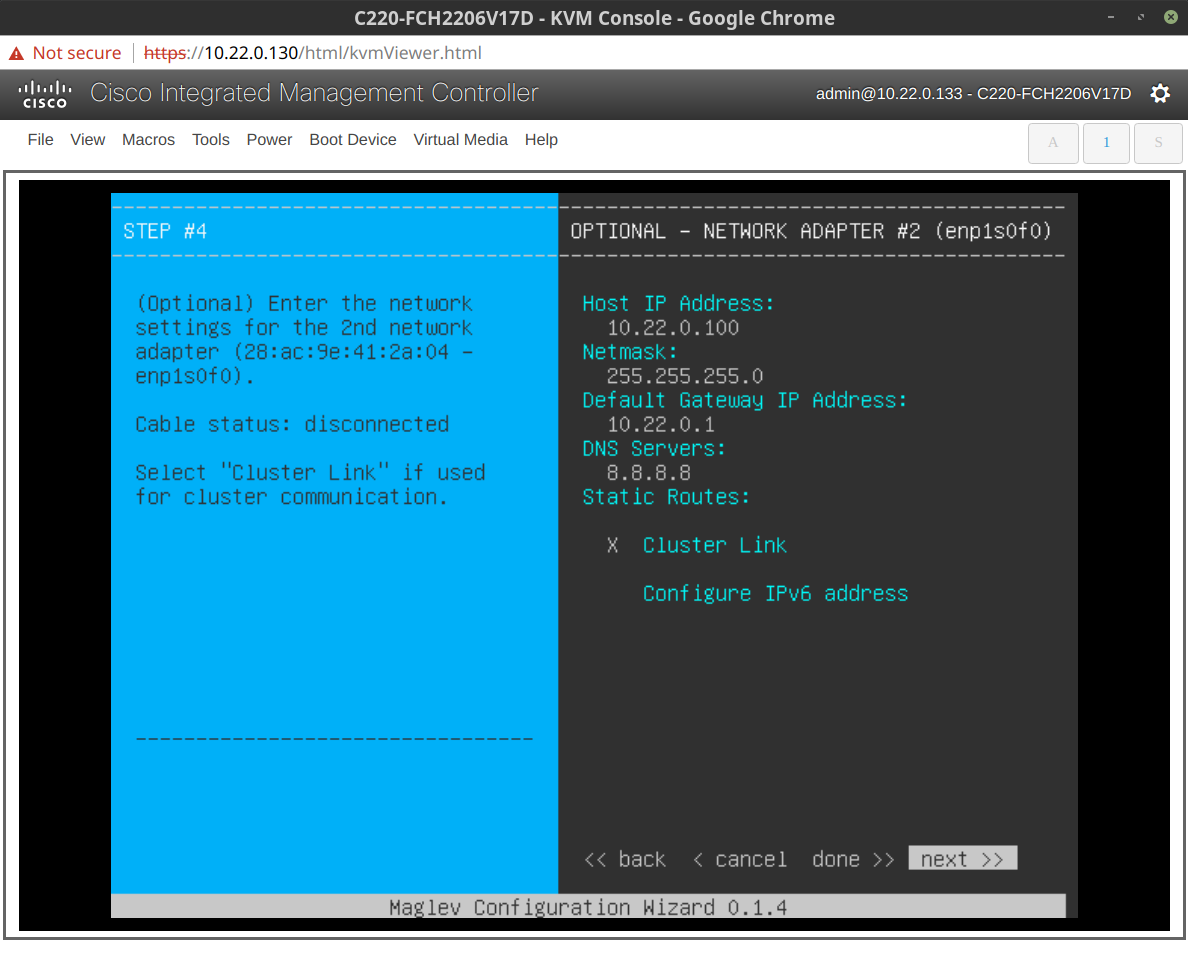
\includegraphics[height=9cm]{img/sc_002.png}
	\caption{DNA Center Configuration Wizard - Entering Management IP}
	\label{fig:dna-center-install-step-4}
\end{figure} 

Im letzten Schritt des Wizards werden alle User Account Einstellungen festgelegt. Hier bei ist zu beachten, dass das "Linux Password" für den SSH Zugriff benötigt wird und die "Administrator Passphrase" für den Zugang zum Web Interface.
 
\begin{figure}[H]
	\centering
	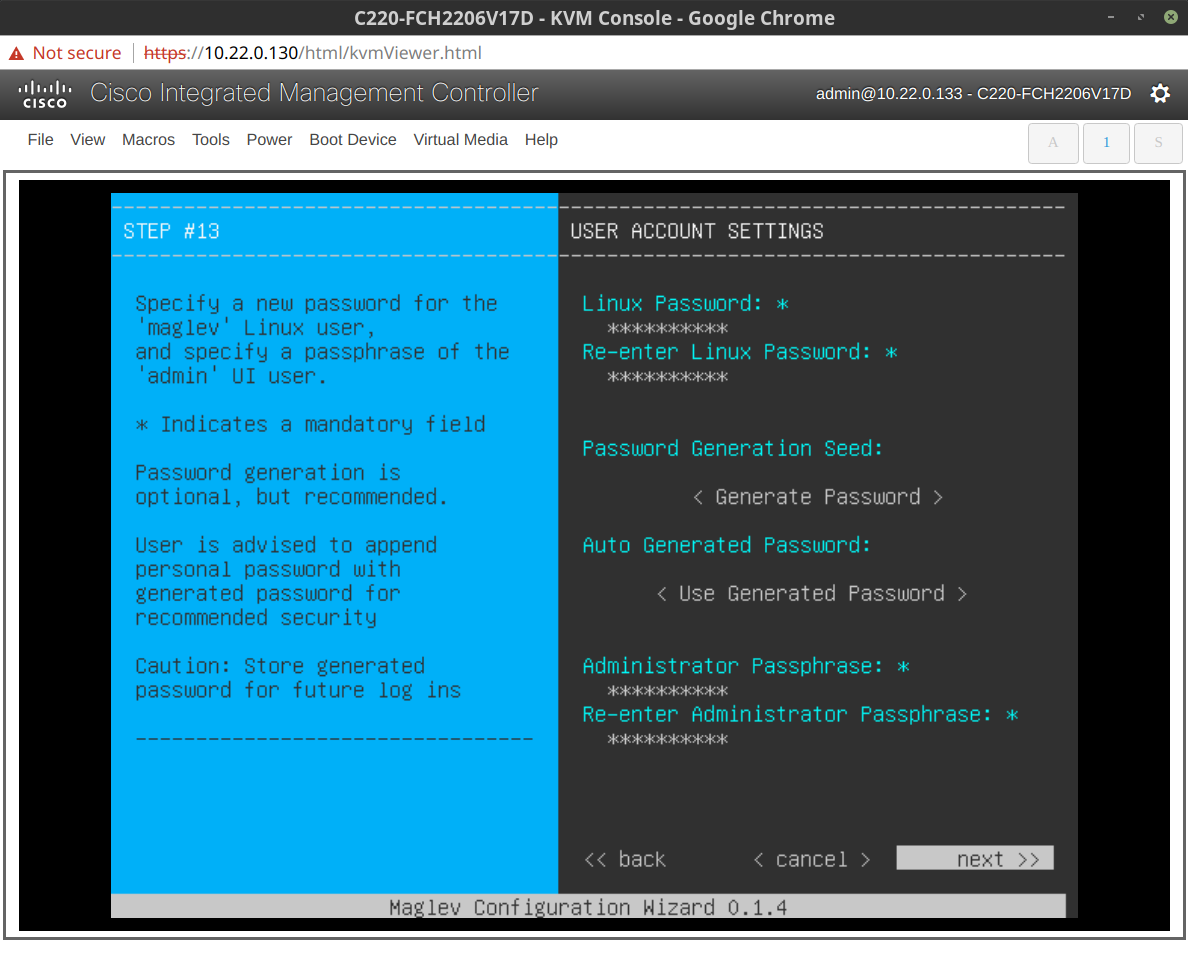
\includegraphics[height=9cm]{img/sc_003.png}
	\caption{DNA Center Configuration Wizard - Entering Authentification Data}
	\label{fig:dna-center-install-step-13}
\end{figure}

Nun wird das DNA Center aufgesetzt. Dieser Prozess dauert mehrere Stunden. 

\begin{figure}[H]
	\centering
	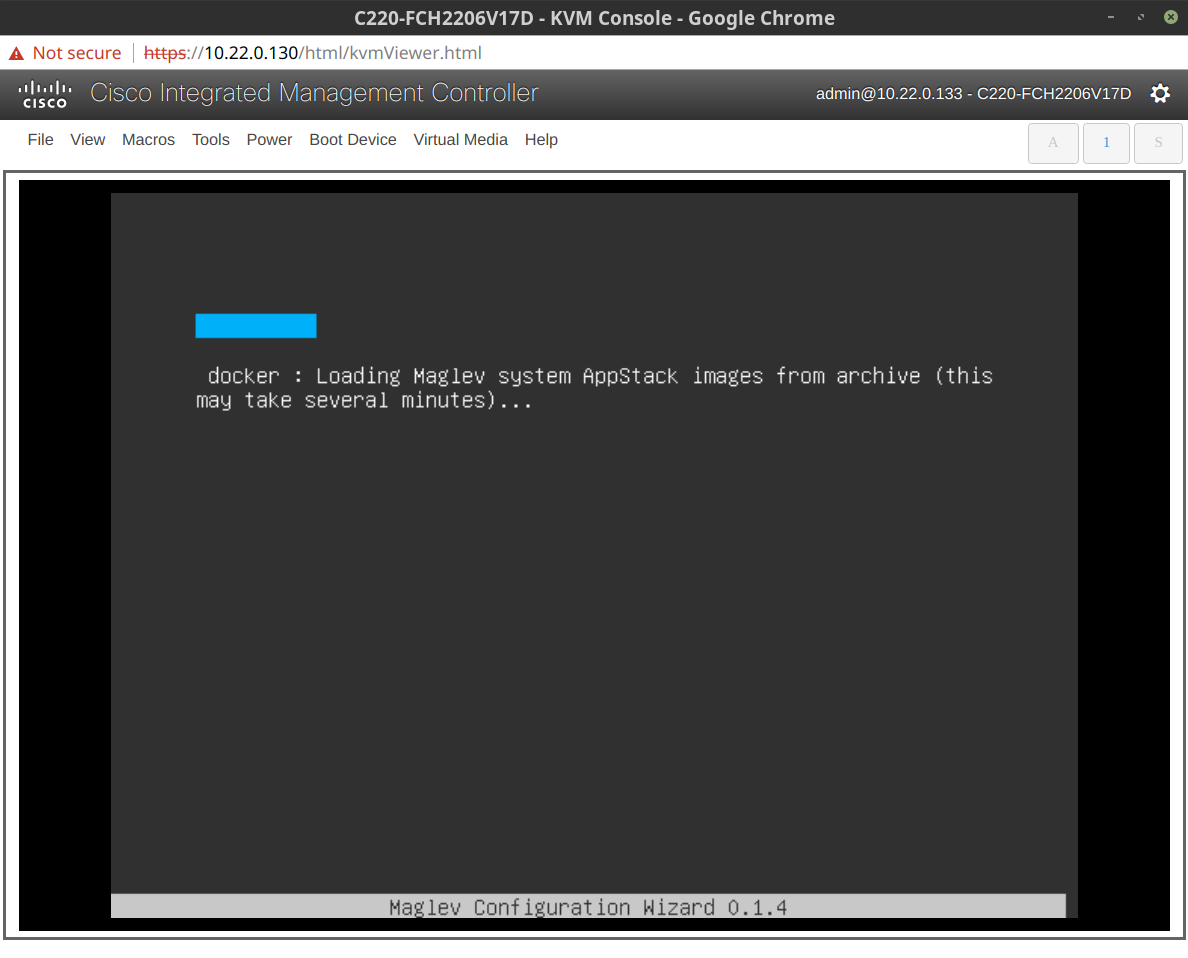
\includegraphics[height=9cm]{img/sc_004.png}
	\caption{DNA Center Configuration Wizard - DNA Center uses docker}
	\label{fig:dna-center-install-step-install}
\end{figure}


\subsubsection{Setup Accounts}
Nach dem der Wizard die Installation vollständig ausgeführt hat, ist das DNA Center Web-GUI verfügbar. Die Konfiguration kann nun über dieses weitergeführt werden.
\begin{figure}[H]
	\centering
	\includegraphics[height=9cm]{img/sc_005.png}
	\caption{DNA Center Web GUI - Login Page}
	\label{fig:dna-center-gui-1}
\end{figure}

Gleich zu Beginn verlangt das DNA Center die Cisco Credentials die mit dem Smart Account verknüpft sind, in welchem die Lizenzen verwaltet werden. Diese Informationen können auch zu einem späteren Zeitpunkt noch eingetragen werden.

\begin{figure}[H]
	\centering
	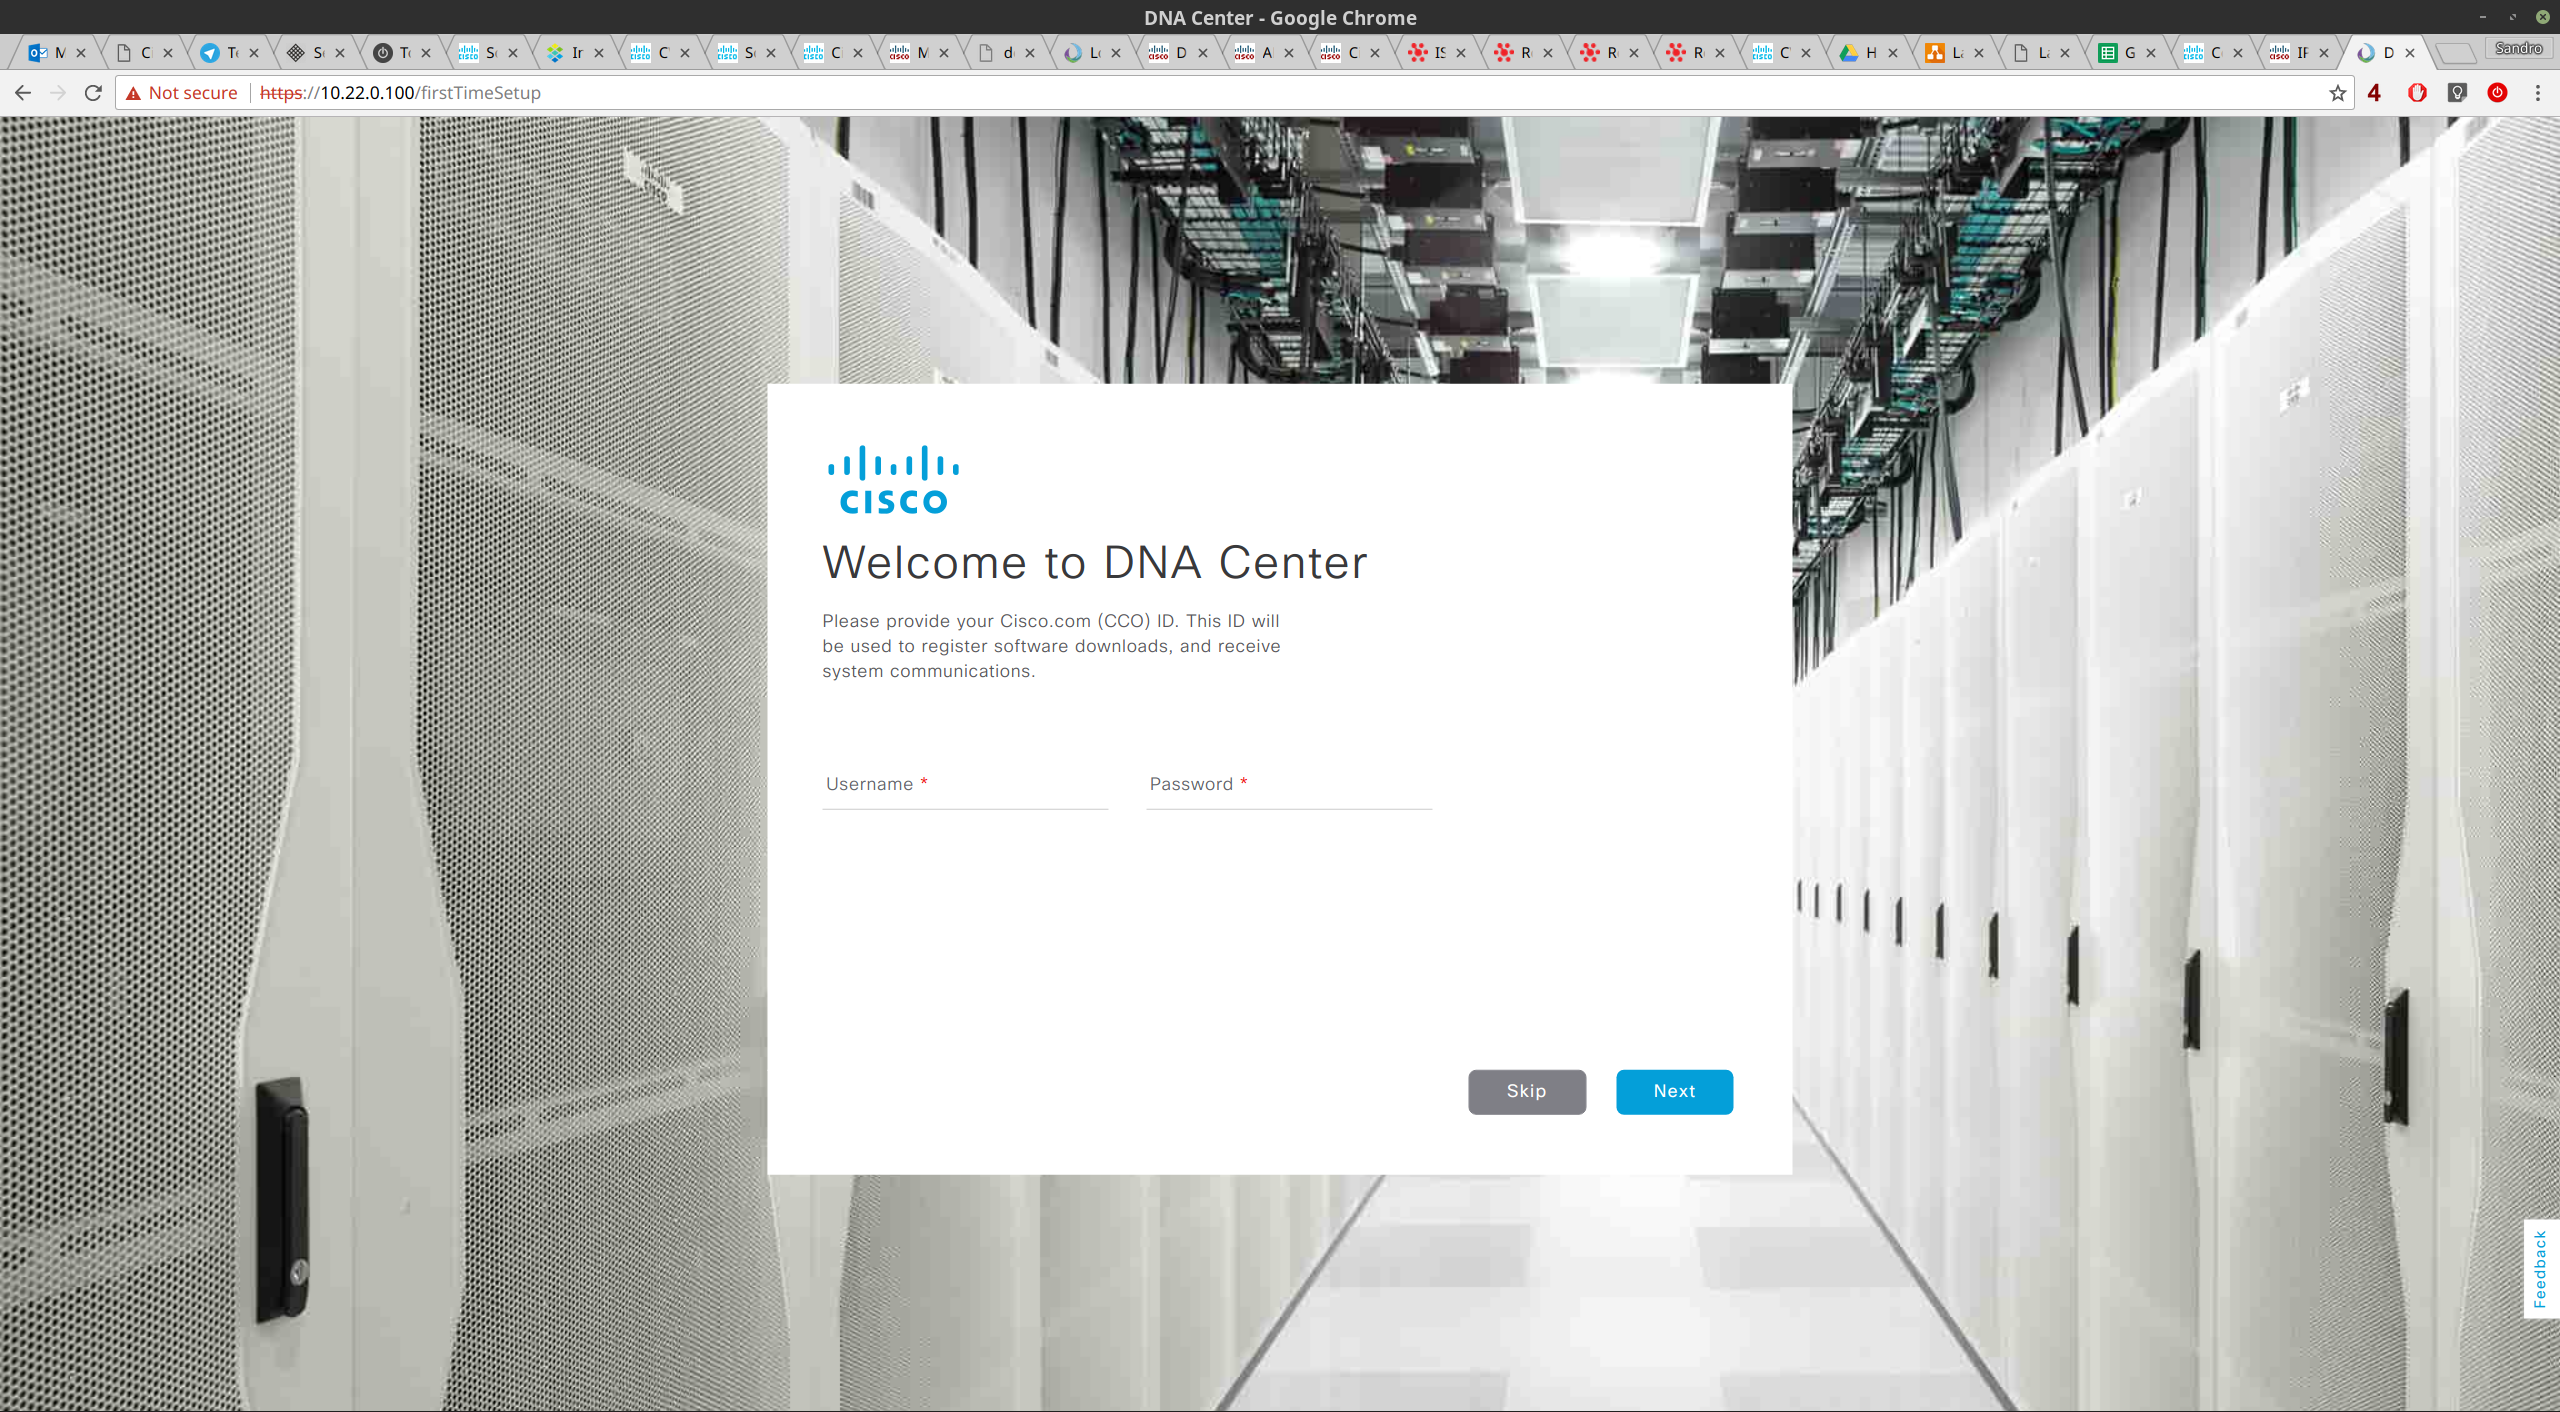
\includegraphics[height=9cm]{img/sc_006.png}
	\caption{DNA Center Web GUI - Cisco Credentials for Licences}
	\label{fig:dna-center-gui-2}
\end{figure}

Im nächsten Schritt kann ein IPAM Server angegeben werden. Diese Einstellung kann ebenfalls später angepasst werden, weshalb wir diesen Schritt zu Beginn übersprungen haben.

\begin{figure}[H]
	\centering
	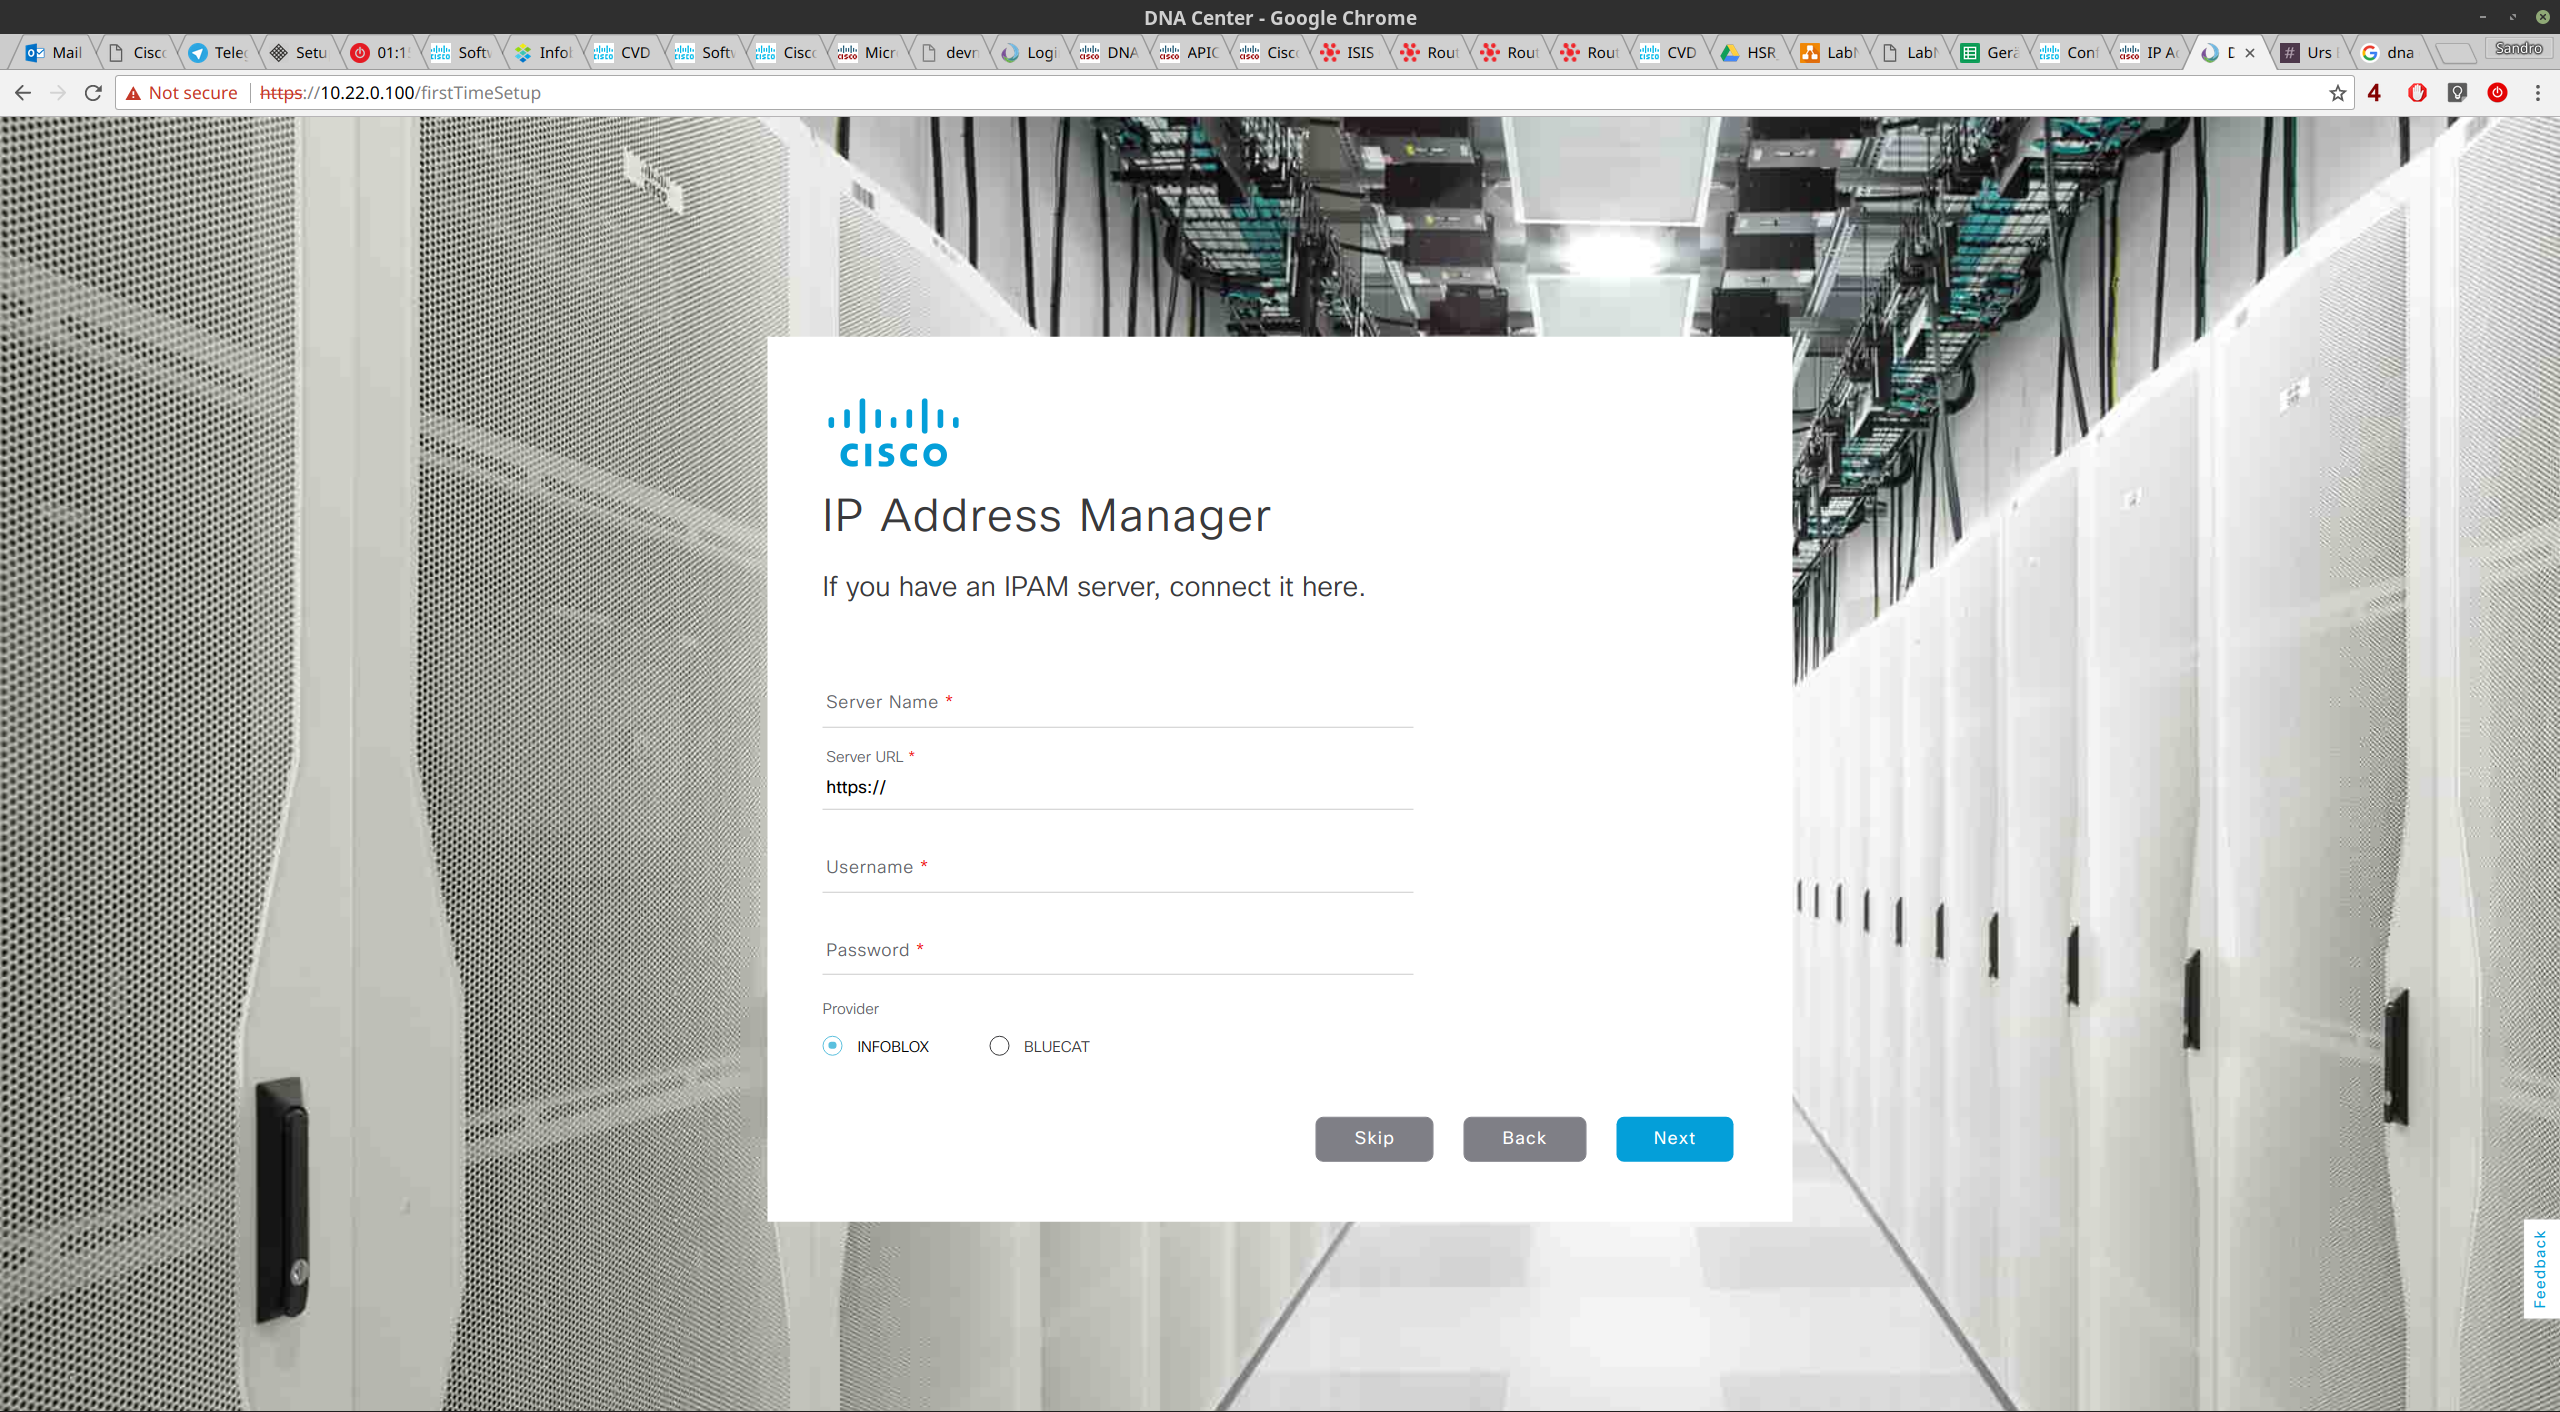
\includegraphics[height=9cm]{img/sc_007.png}
	\caption{DNA Center Web GUI - Cisco IPAM}
	\label{fig:dna-center-gui-3}
\end{figure}

Danach ist die initiale Konfiguration beendet und das DNA Center Dashboard wird angezeigt.

\begin{figure}[H]
	\centering
	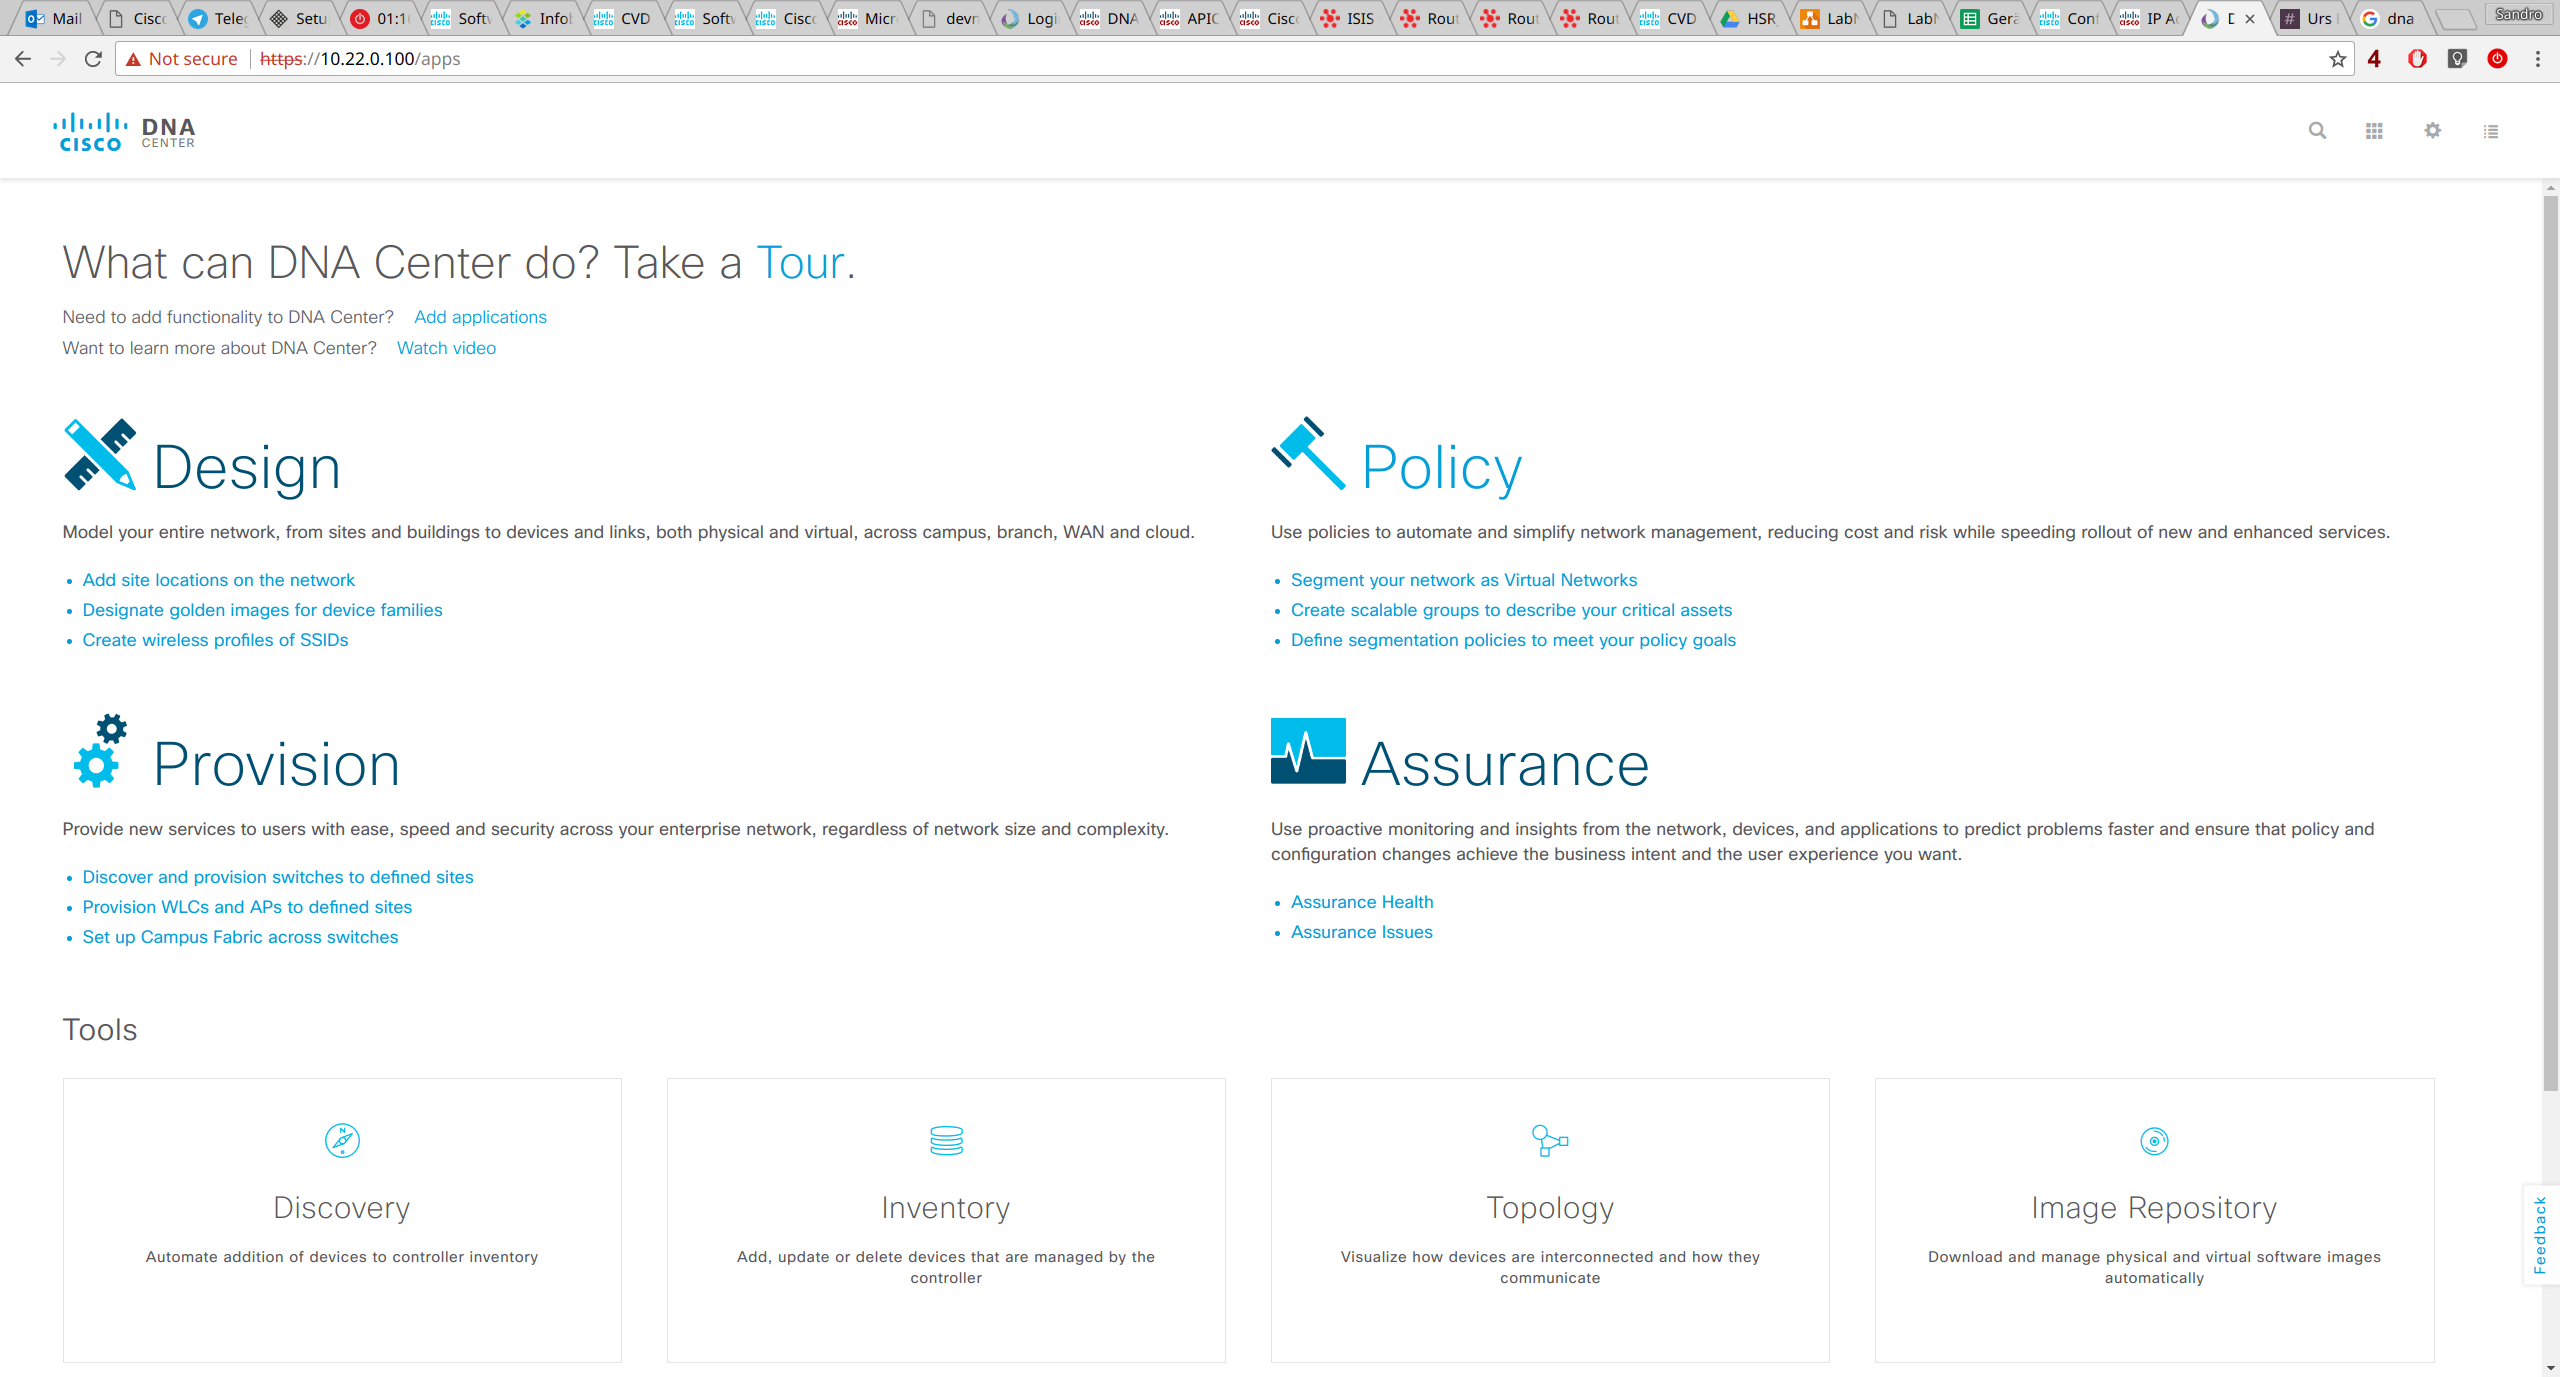
\includegraphics[height=9cm]{img/sc_008.png}
	\caption{DNA Center Web GUI - Dashboard}
	\label{fig:dna-center-gui-4}
\end{figure}

\subsection{DNA Center Updates}
Da sich das DNA Center während dem Setup Prozess nicht automatisch aktualisiert und die DNA Center in relativ kurzen Intervallen released werden, ist es ratsam, gleich zu Beginn die aktuellsten Updates zu installieren.

Der Updateprozess birgt jedoch einige Hürden:
\begin{itemize}
	\item System Updates müssen vor den Package Updates installiert werden.
	\item Werden die Package Updates vor dem System Update ausgeführt, können diese blockieren. 
	\item Die Package Updates müssen in der richten Reihenfolge installiert werden.
	\item Die oben genannte Reihenfolge ist nicht direkt ersichtlich.
	\item Der Updatevorgang dauert mehrere Stunden.
	\item Der Updatefortschritt wird nicht angezeigt. 
	\item Während dem Updateprozess können Teile des Web-GUIs Fehlermeldungen anzeigen oder überhaupt nicht mehr erreichbar sein.\\
\end{itemize} 

Die Update Ansicht ist unter \textit{Einstellungen (Zahnrad-Symbol) $\rightarrow$ System Settings  $\rightarrow$ App Management} zu finden:

\begin{figure}[H]
	\centering
	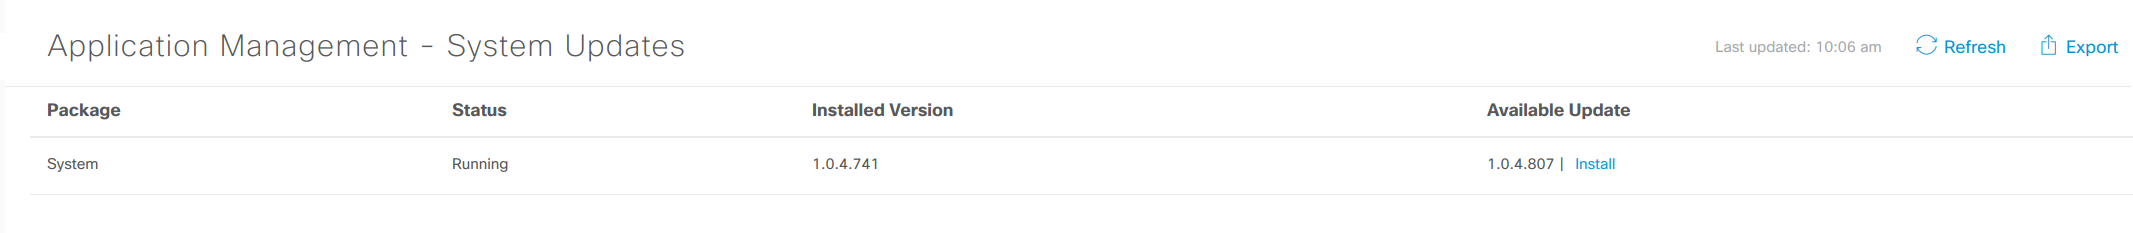
\includegraphics[width=\columnwidth]{img/sc_009.png}
	\caption{DNA Center App Management}
	\label{fig:dna-center-gui-update-1}
\end{figure}

\subsubsection{Fehlgeschlagene Updates reparieren}
Abgestürzte Packete können mit den folgenden Befehlen wieder repariert werden (am Beispiel von main-system-package:1.0.4.779):

\begin{lstlisting}[language=bash]
$ maglev package status | awk  '$3 ~ /[0-9]+/ {print $1":"$3}' | 
grep -v "^system" |  while read pkg; 
do maglev catalog package delete $pkg;done
$ maglev system_update_package install main-system-package:1.0.4.779
\end{lstlisting}

\subsubsection{Update Reihenfolge}
Nach einem Update wurde die Reihenfolge von System und Package Update angepasst. Vermutlich um den Administrator dazu zu bringen zuerst die System Updates zu installieren. 

\begin{figure}[H]
	\centering
	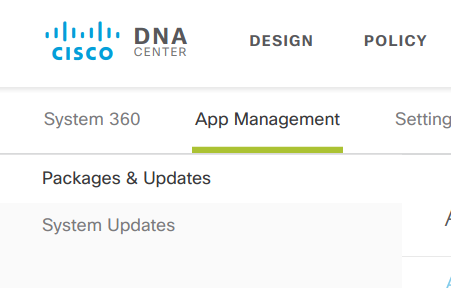
\includegraphics[height=4cm]{img/sc_010.png}
	\caption{DNA Center App Management - Alte Menü Anordnung}
	\label{fig:dna-center-gui-update-2}
\end{figure}

\subsubsection{Schwierigkeit: Cisco CCO Login für Updates notwendig}

Application Packages und System Updates können nur installiert werden, wenn die Cisco CCO Credentials hinterlegt sind.

\begin{figure}[H]
	\centering
	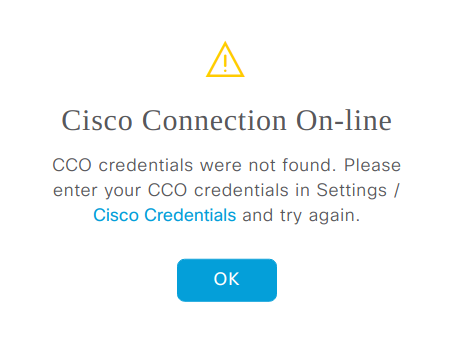
\includegraphics[height=4cm]{img/dan-center-cisco-credentials-required.png}
	\caption{DNA Center Upgrade - Cisco Credentials required}
	\label{fig:dna-center-cisco-credentials-required}
\end{figure}

\subsubsection{Schwierigkeit: Unterschiedliche Versionsangabe}

Beim Updatevorgang kann es zu Verwirrungen kommen, weil die Versionangabe von der Funktion \textit{About} von der Version des System Packages abweicht.

\begin{figure}[H]
	\centering
	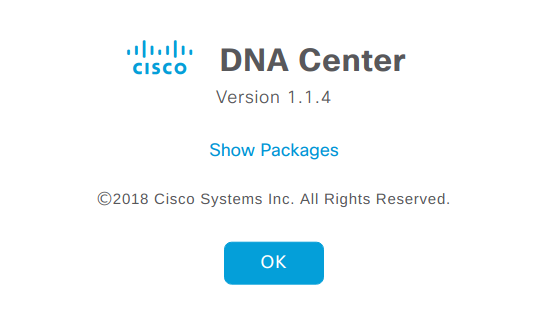
\includegraphics[height=3cm]{img/dna-center-about.png}
	\caption{DNA Center - About - Version}
	\label{fig:dna-center-about}
\end{figure}

Oben wurde bei \textit{About} die richtige Version 1.1.4 angegeben. Nachfolgend die Anzeige unter \textit{System Updates}, welche eine andere Version anzeigt.
\begin{figure}[H]
	\centering
	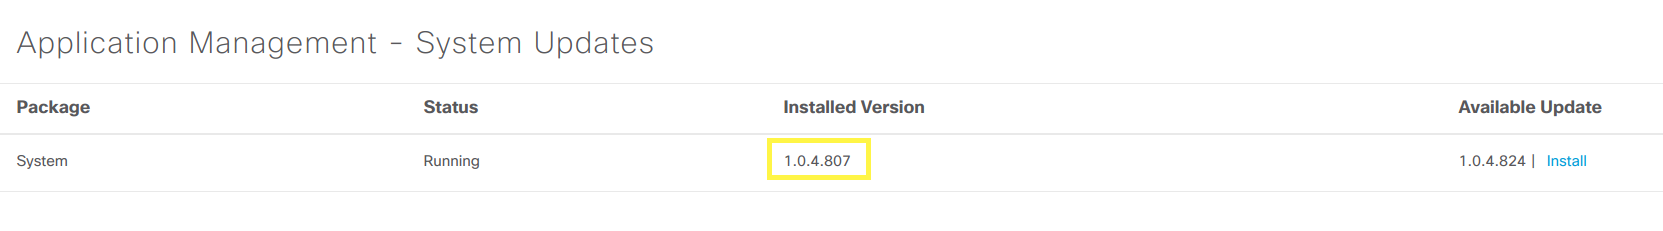
\includegraphics[height=2.25cm]{img/dna-center-system-upgrade-version.png}
	\caption{DNA Center - System Upgrade - Version}
	\label{fig:dna-center-system-upgrade}
\end{figure}

\subsection{Cisco PNP mit DNA Center}
DNA Center hat Plug and Play als App und nutzt diese um voll automatisch einen Switch/Router zu konfigurieren. 
\subsubsection{DHCP Konfiguration}
Bei unserem ersten Versuch ein Seed-Device festzulegen, wurde vom DNA-C kein DHCP Server konfiguriert, weshalb wir dies manuell auf Infoblox eingerichtet haben.
 
\begin{itemize}
	\item DNA Center akzeptiert Cisco PNP Anfragen via http
	\item Cisco Switches/Router versuchen beim ersten Boot ohne eine Konfiguration DHCP und Cisco PNP auszuführen
\end{itemize}

Die Cisco PNP Discovery kann über die DHCP Optione 43 und 60 konfiguriert werden (siehe \cite{cisco-pnp-dhcp}). In unserem Fall haben wir diese Optionen wie nachfolgend auf der Grafik erischtlich auf dem Infoblox Server konfiguriert.

\begin{figure}[H]
	\centering
	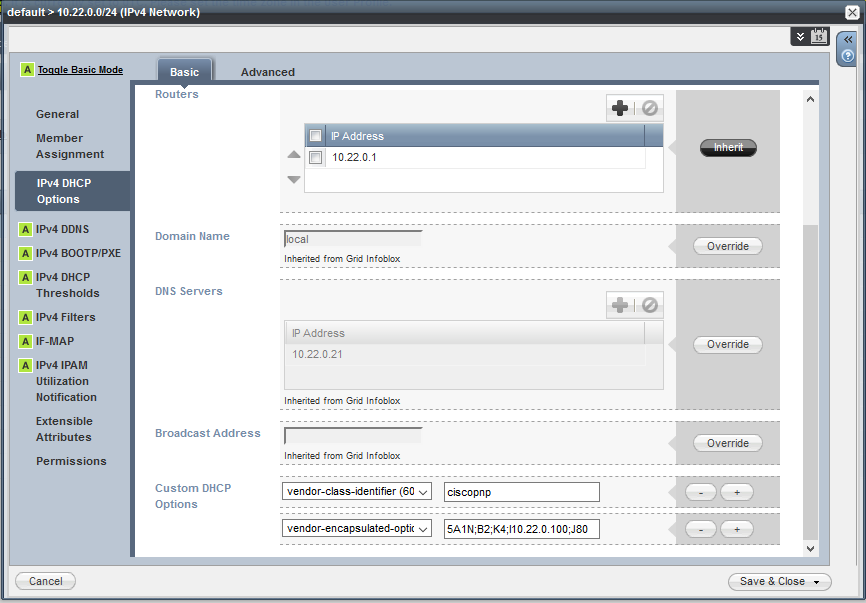
\includegraphics[height=10cm]{img/Infoblox_PNP.png}
	\caption{Infoblox Cisco PNP DHCP Option Konfiguration}
	\label{fig:cisco-pnp}
\end{figure}

\subsection{ISIS Konfiguration}
Da die automatische Erstellung des Underlay Netzwerkes mit der LAN-Automation Funktion nicht funktionierte, mussten wir dieses selber Konfigurieren. 

\subsection{Automatischer "Claim" von Netzwerkgeräten}

\subsubsection{DNA Center Provision - Unclaimed Devices}

Nachdem die DHCP Option erfolgreich konfiguriert ist, werden die Geräte vom DNA-C gefunden und erscheinen Geräte im Device Inventory.

\begin{figure}[H]
	\centering
	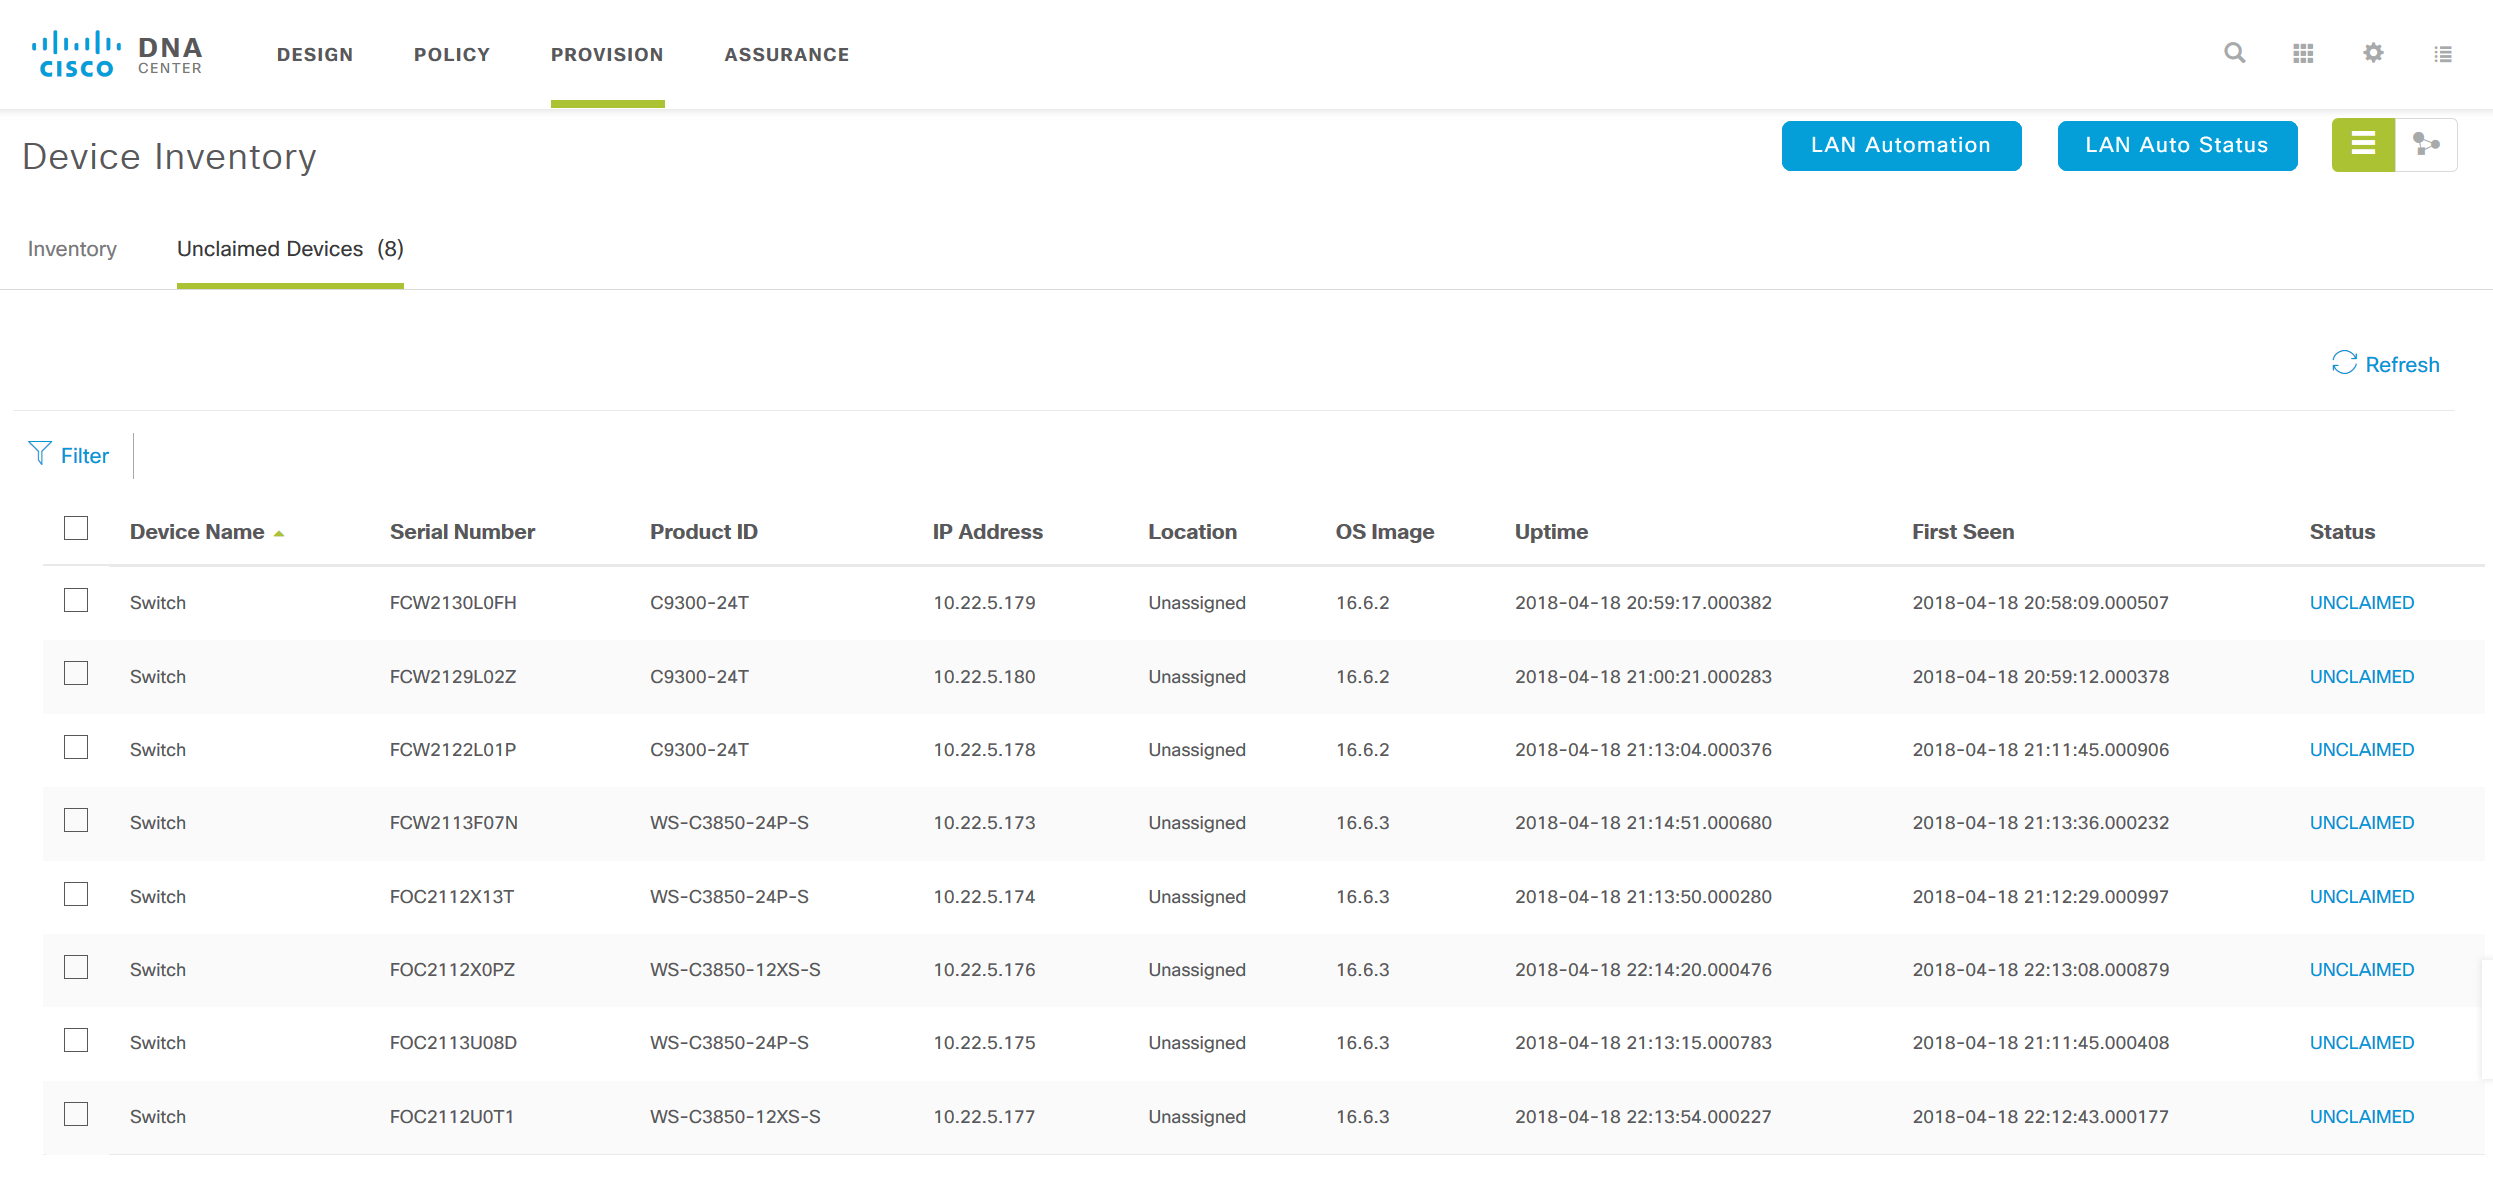
\includegraphics[height=8cm]{img/DNA_Center_All_Fabric2_Unclaimed.PNG}
	\caption{DNA Center Provision - Alle Geräte erfolgreich in der "Unclaimed List"}
	\label{fig:dna-center-provision-unclaimed}
\end{figure}

Bevor es jedoch so weit kam, wurden verschiedene Fehlermeldungen angezeigt. Diese konnten jeweils behoben werden indem das betroffene Gerät auf Werkeinstellung zurückgesetzt und neu gestartet wurde. Dieser Vorgang wurde so lange wiederholt bis keine Fehlermeldungen mehr angezeigt wurden. 

\begin{figure}[H]
	\centering
	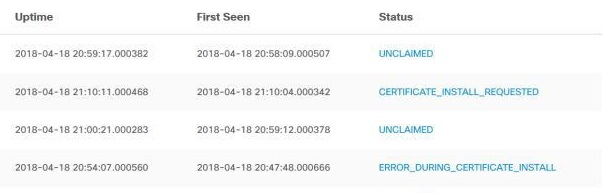
\includegraphics[height=4cm]{img/DNA_Center_Unclaimed_Errors_1.PNG}
	\caption{DNA Center Provision - Fehlermeldungen in der "Unclaimed List"}
	\label{fig:dna-center-provision-unclaimed-2}
\end{figure}

\subsection{DNA Center Netzwerk Design}

\subsubsection{Network Hierarchy}

Gemäss unserer Netzwerk Architektur wie in Kapitel \ref{fig:LabNetworkArchitecture} beschrieben, haben wir zwei Standorte. Rapperswil mit zwei Gebäuden und Jona mit einem Gebäude.
In DNA Center können diese sehr einfach im Abschnitt \textit{Design $\rightarrow$ Network Hierarchy} hinzugefügt werden. Seltsamer Weise ist in den Angaben die Adresse nur optional, dafür aber die Koordinaten der Breiten- und Längengrade Pflicht.

\begin{figure}[H]
	\centering
	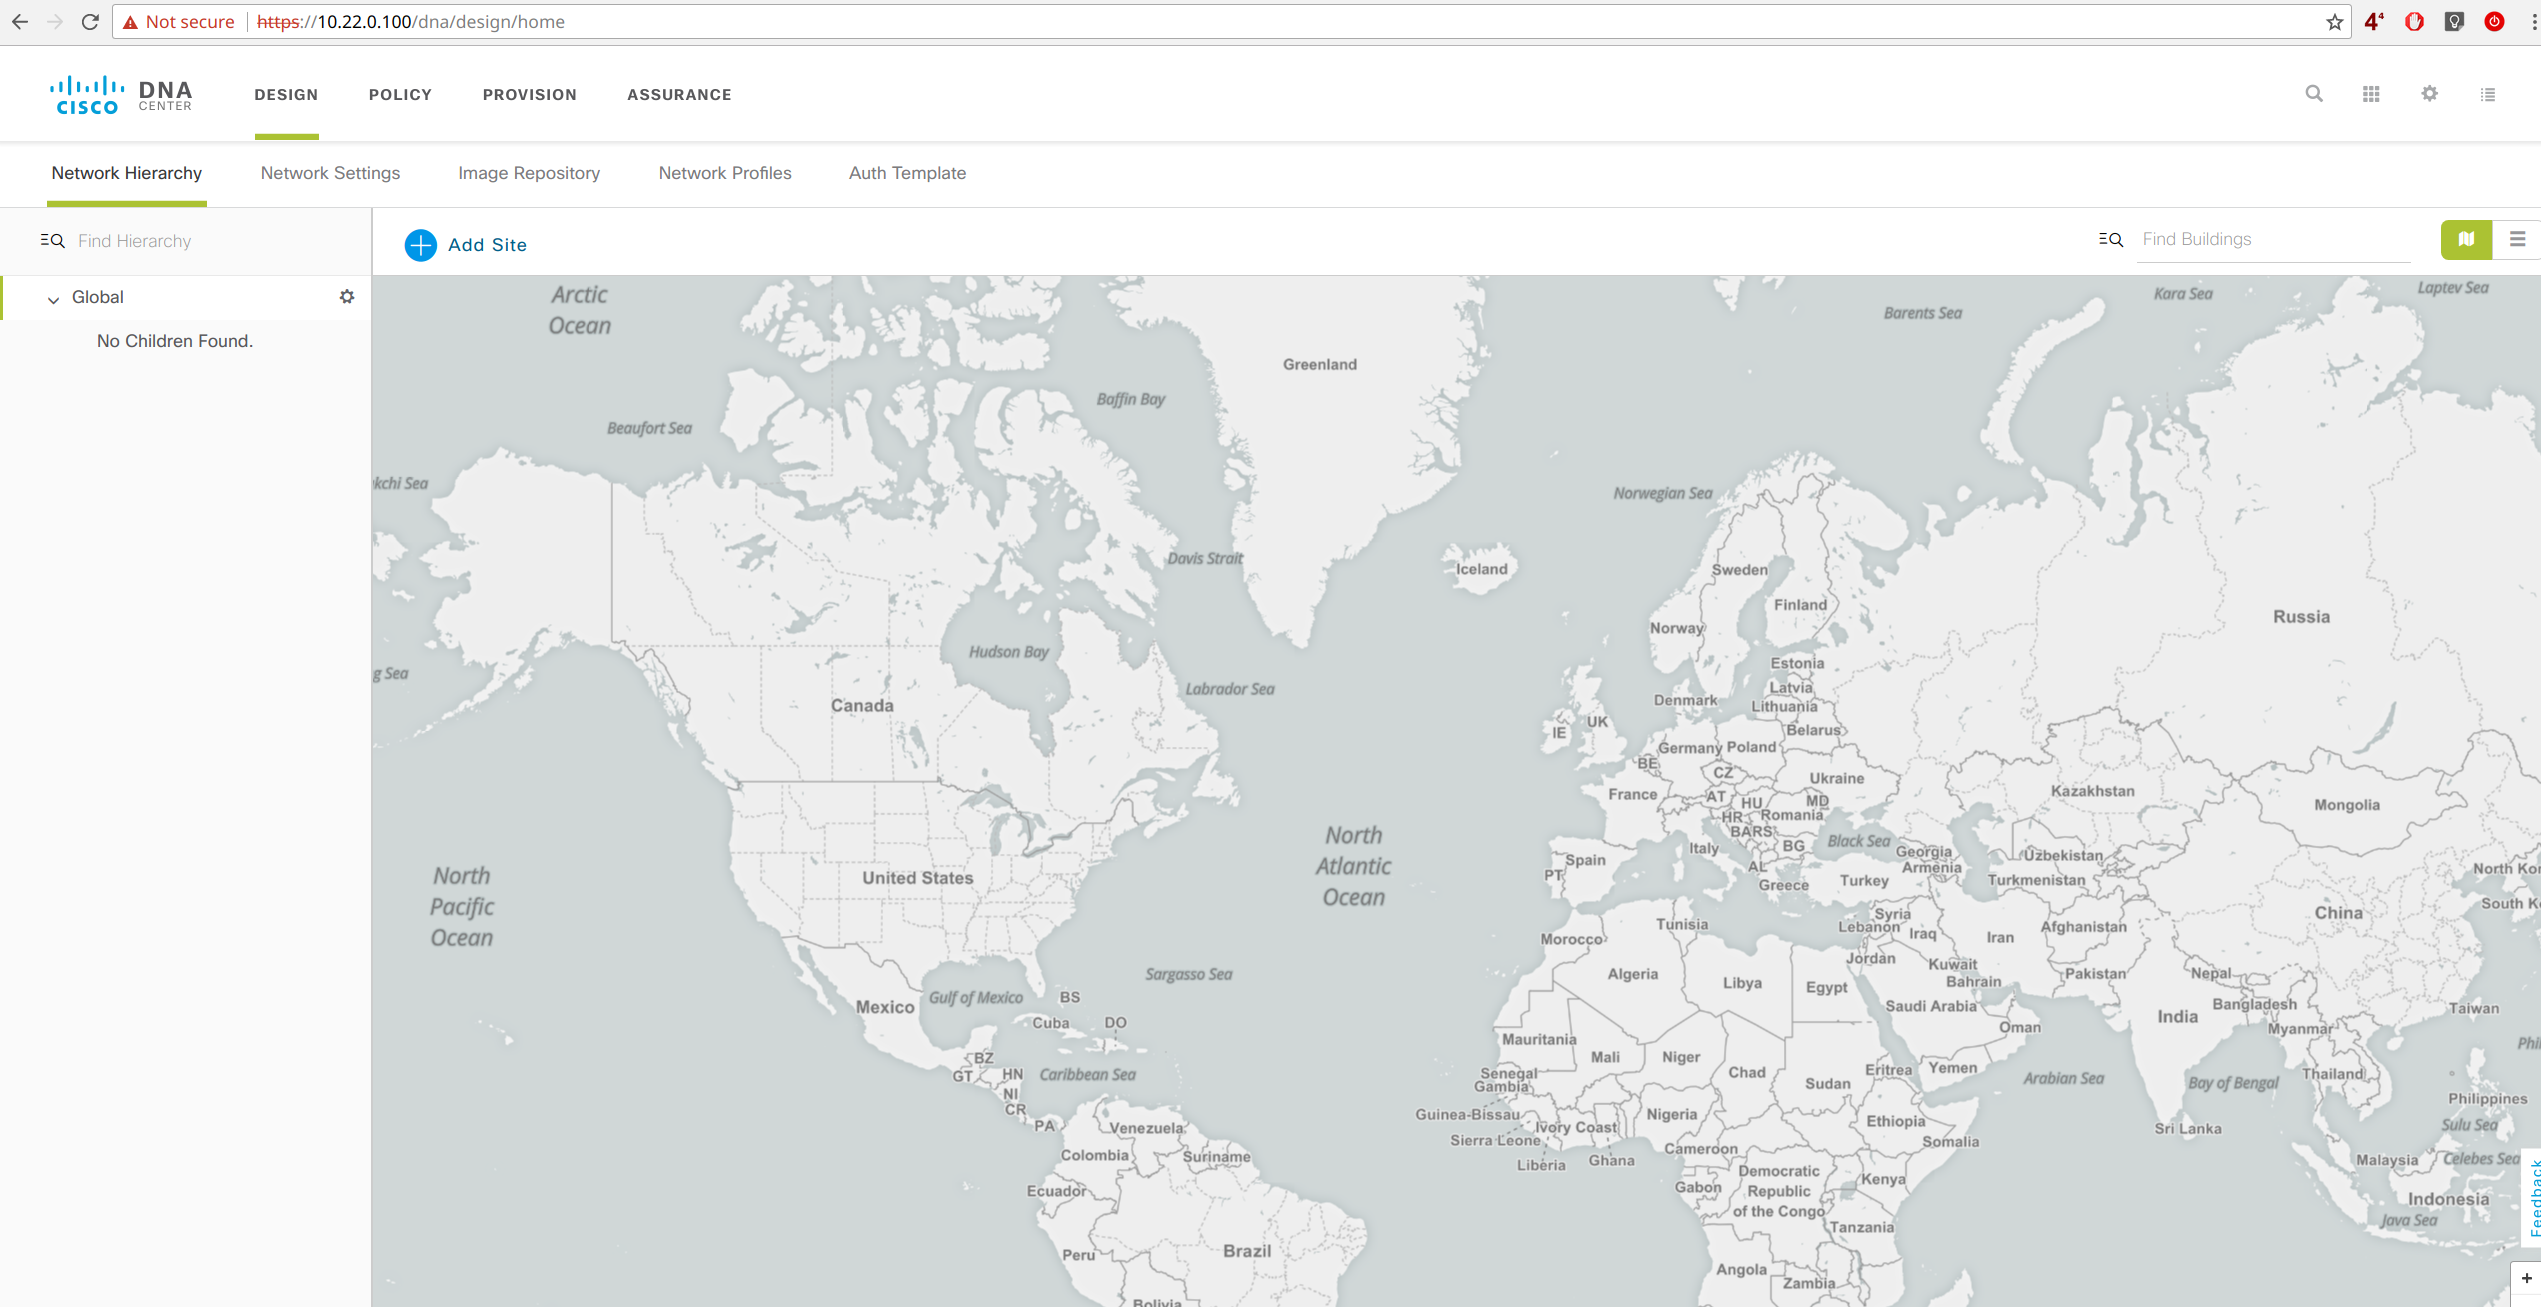
\includegraphics[height=8cm]{img/Selection_011.png}
	\caption{DNA Center Design Map}
	\label{fig:dna-center-design-1}
\end{figure}

\begin{figure}[H]
	\centering
	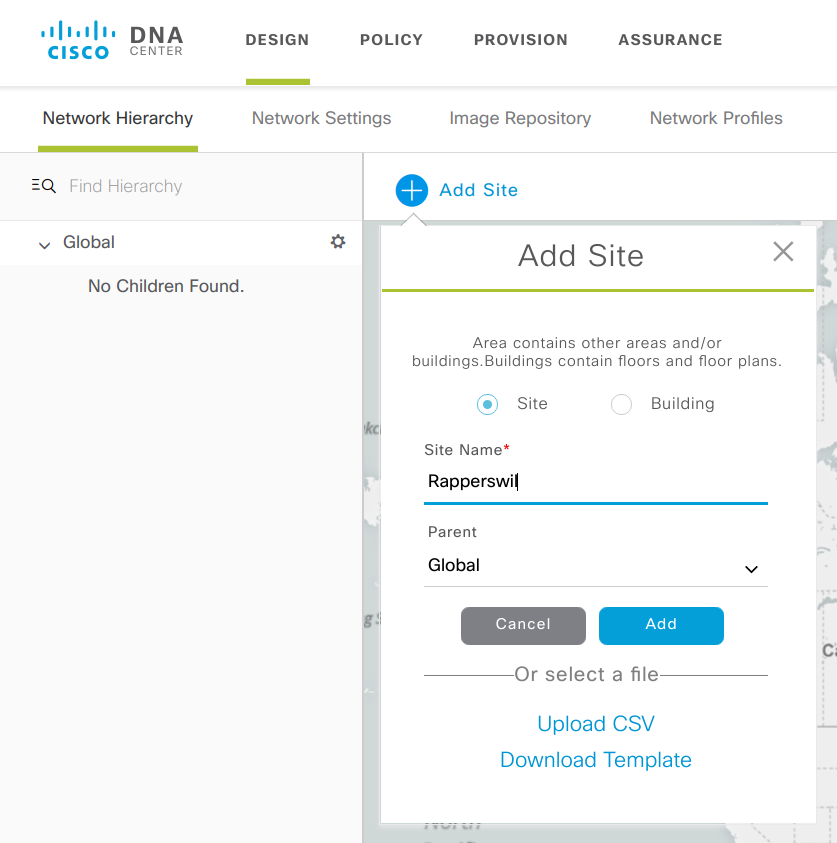
\includegraphics[height=6cm]{img/Selection_012.png}
	\caption{DNA Center Design - Standort hinzufügen}
	\label{fig:dna-center-design-2}
\end{figure}

\begin{figure}[H]
	\centering
	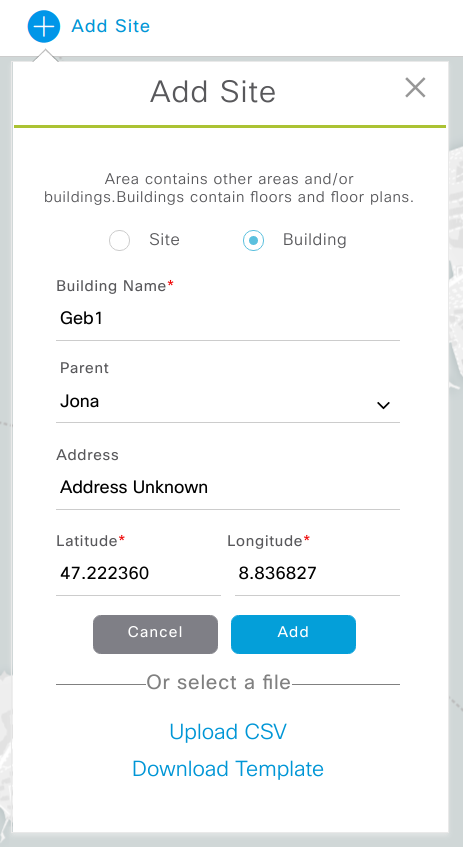
\includegraphics[height=6cm]{img/Selection_014.png}
	\caption{DNA Center Design - Gebäude können mit Koordinaten hinzugefügt werden.}
	\label{fig:dna-center-design-3}
\end{figure}

\begin{figure}[H]
	\centering
	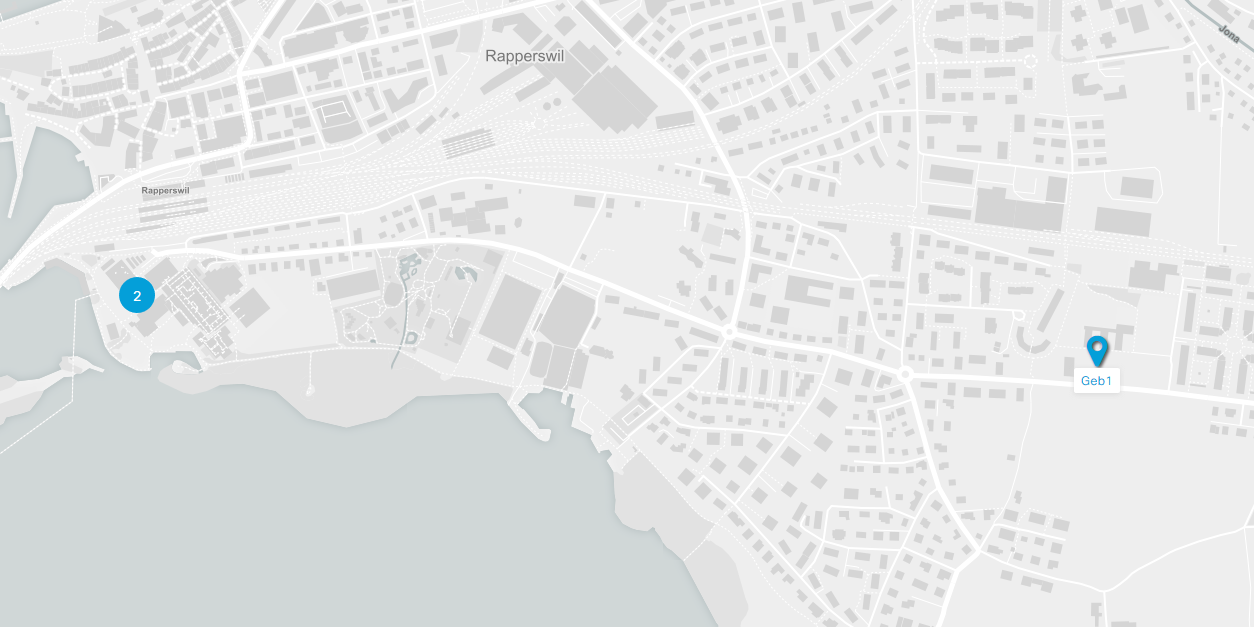
\includegraphics[height=8cm]{img/design_map_overview.PNG}
	\caption{DNA Center Design - Übersicht über alle Standorte und Gebäude}
	\label{fig:dna-center-design-overview}
\end{figure}

\subsection{Netzwerkgeräte zu Inventory hinzufügen}


\subsubsection{Manuell Geräte im DNA Center hinzufügen}
Da alle Versuche die Geräte automatisch hinzuzufügen gescheitert sind, entschieden wir uns den Vorgang manuell durchzuführen. 

Im Dashboard klickt man dazu auf \textit{Inventory} (siehe \ref{fig:dna-center-inventory-button})

\begin{figure}[H]
	\centering
	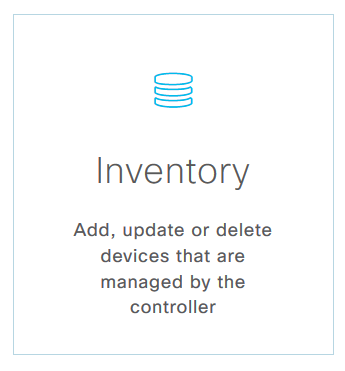
\includegraphics[height=3cm]{img/dna-center-inventory-button.PNG}
	\caption{DNA Center Dashboard - Inventory Knopf}
	\label{fig:dna-center-inventory-button}
\end{figure}

Anschliessend wählt man \textit{Add} (siehe \ref{fig:dna-center-inventory-add})

\begin{figure}[H]
	\centering
	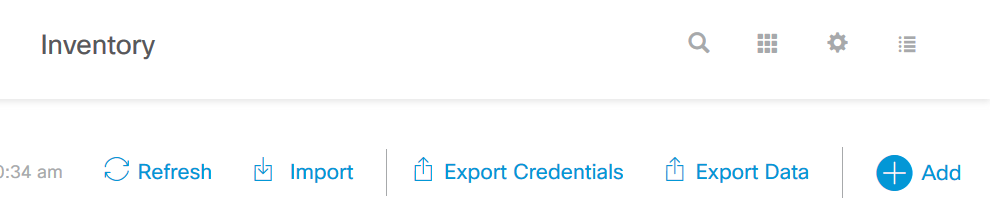
\includegraphics[height=3cm]{img/dna-center-inventory-add.PNG}
	\caption{DNA Center Inventory - Gerät hinzufügen}
	\label{fig:dna-center-inventory-add}
\end{figure}

Anschliessend müssen folgende Informationen eingegeben werden:
\begin{itemize}
	\item Device Type
	\item Device IP \ Name
	\item SNMP (Version, Read und Write Community)
	\item CLI (via SSH oder Telnet) \textit{oder}
	\item NETCONF
\end{itemize}

Wir entschieden uns CLI via SSH zu nehmen. Von NETCONF und CLI muss nur eine von beiden Optionen gewählt werden. 

\begin{figure}[H]
	\centering
	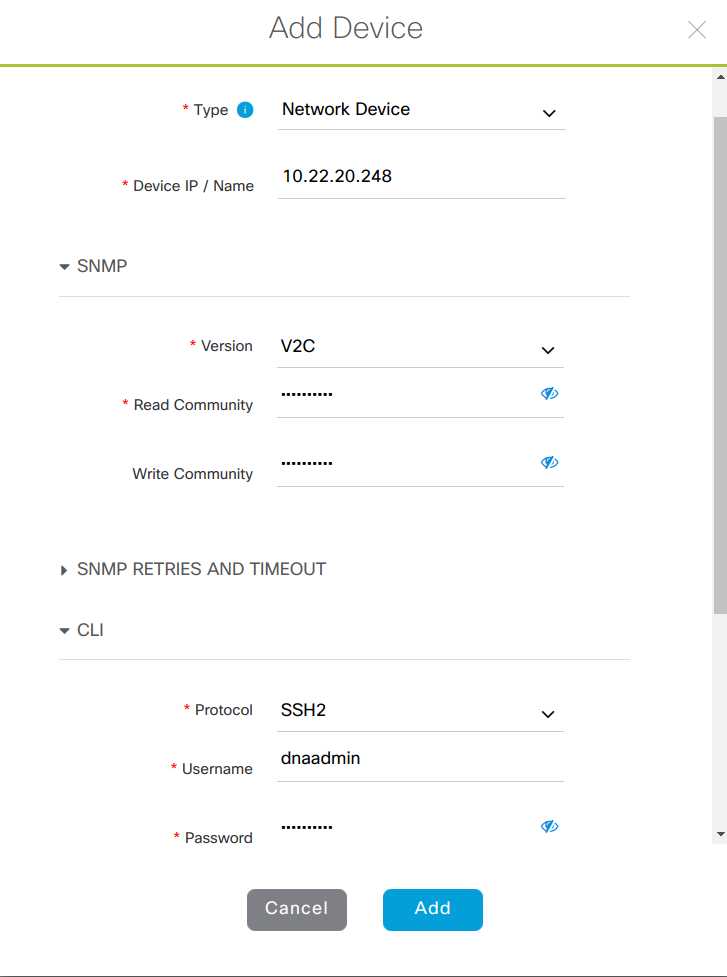
\includegraphics[height=5cm]{img/dna-center-inventory-add-form.png}
	\caption{DNA Center Inventory - Formular Gerät hinzufügen}
	\label{fig:dna-center-inventory-add-form}
\end{figure}

Danach erscheint das Gerät im Inventory. (siehe \ref{fig:dna-center-inventory-index-new})

\begin{figure}[H]
	\centering
	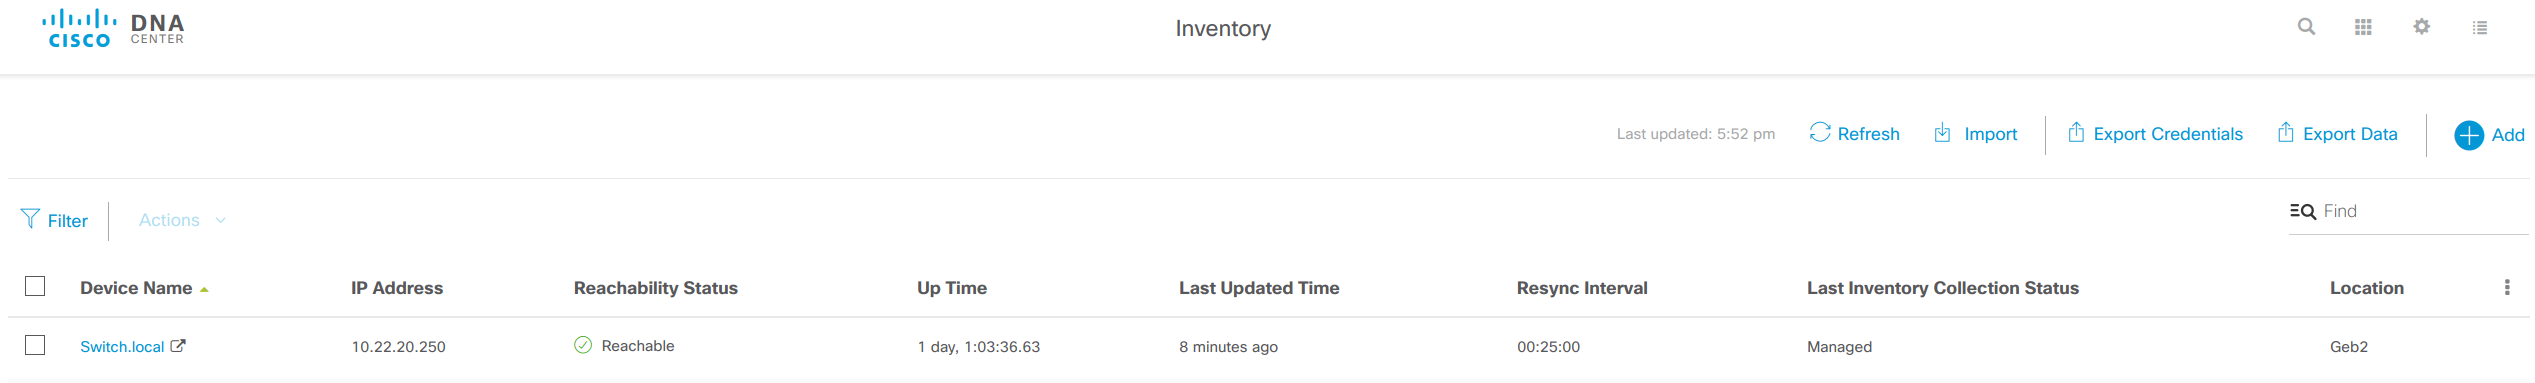
\includegraphics[height=2cm]{img/dna-center-inventory-index-new.png}
	\caption{DNA Center Inventory - Neue Geräte in der Liste}
	\label{fig:dna-center-inventory-index-new}
\end{figure}


\subsection{Image Repository}
Im DNA Center können Netzwerkgeräte automatisch aktualisiert werden. Sobald ein Gerät im Inventory erfolgreich hinzugefügt worden ist, sucht das DNA Center nach Updates. Allerdings nur, wenn ein CCO Account konfiguriert ist. Die Verfügbaren Images sind unter \textit{Desing $\rightarrow$ Global $\rightarrow$ Image Repository} zu finden.

\begin{figure}[H]
	\centering
	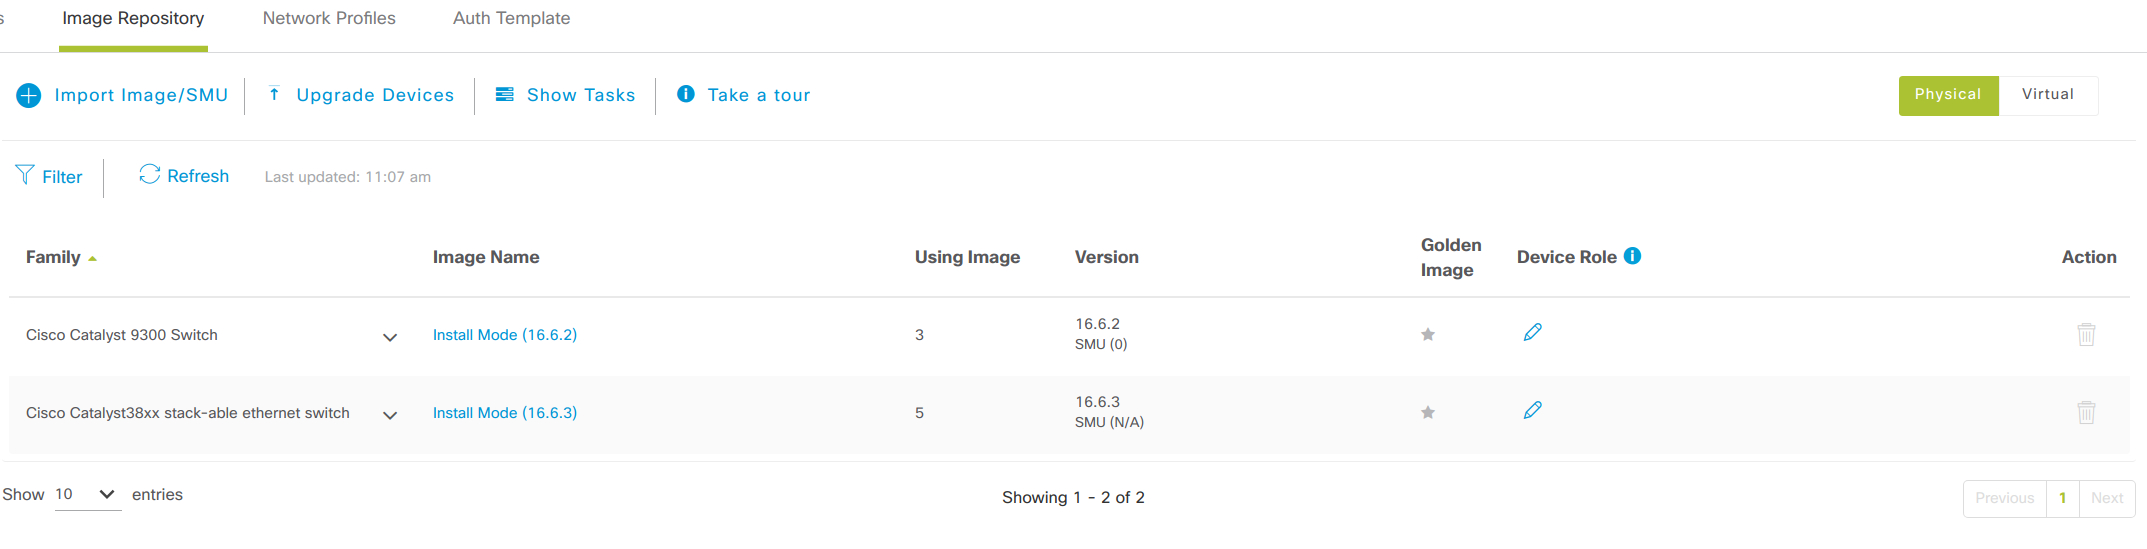
\includegraphics[height=2cm]{img/dna-center-design-image-repository.png}
	\caption{DNA Center Design - Image Respository}
	\label{fig:dna-center-design-image-repository}
\end{figure}

In diesem Image Repository können neue Images heruntergeladen und die gewünschte Version kann mit dem Golden Tag versehen werden. 

\subsection{Automatisches Softwareupdate von Netzwerkgeräten}
Die Softwareupdates von Netzwerkgeräten können im DNA-C unter \textit{Provision $\rightarrow$ devices $\rightarrow$ Inventory} durchgeführt werden. Ebenfalls wird hier automatisch angezeigt, welche Softwareversion zur Zeit auf dem Gerät installiert und ob diese aktuell oder outdated ist.

\begin{figure}[H]
	\centering
	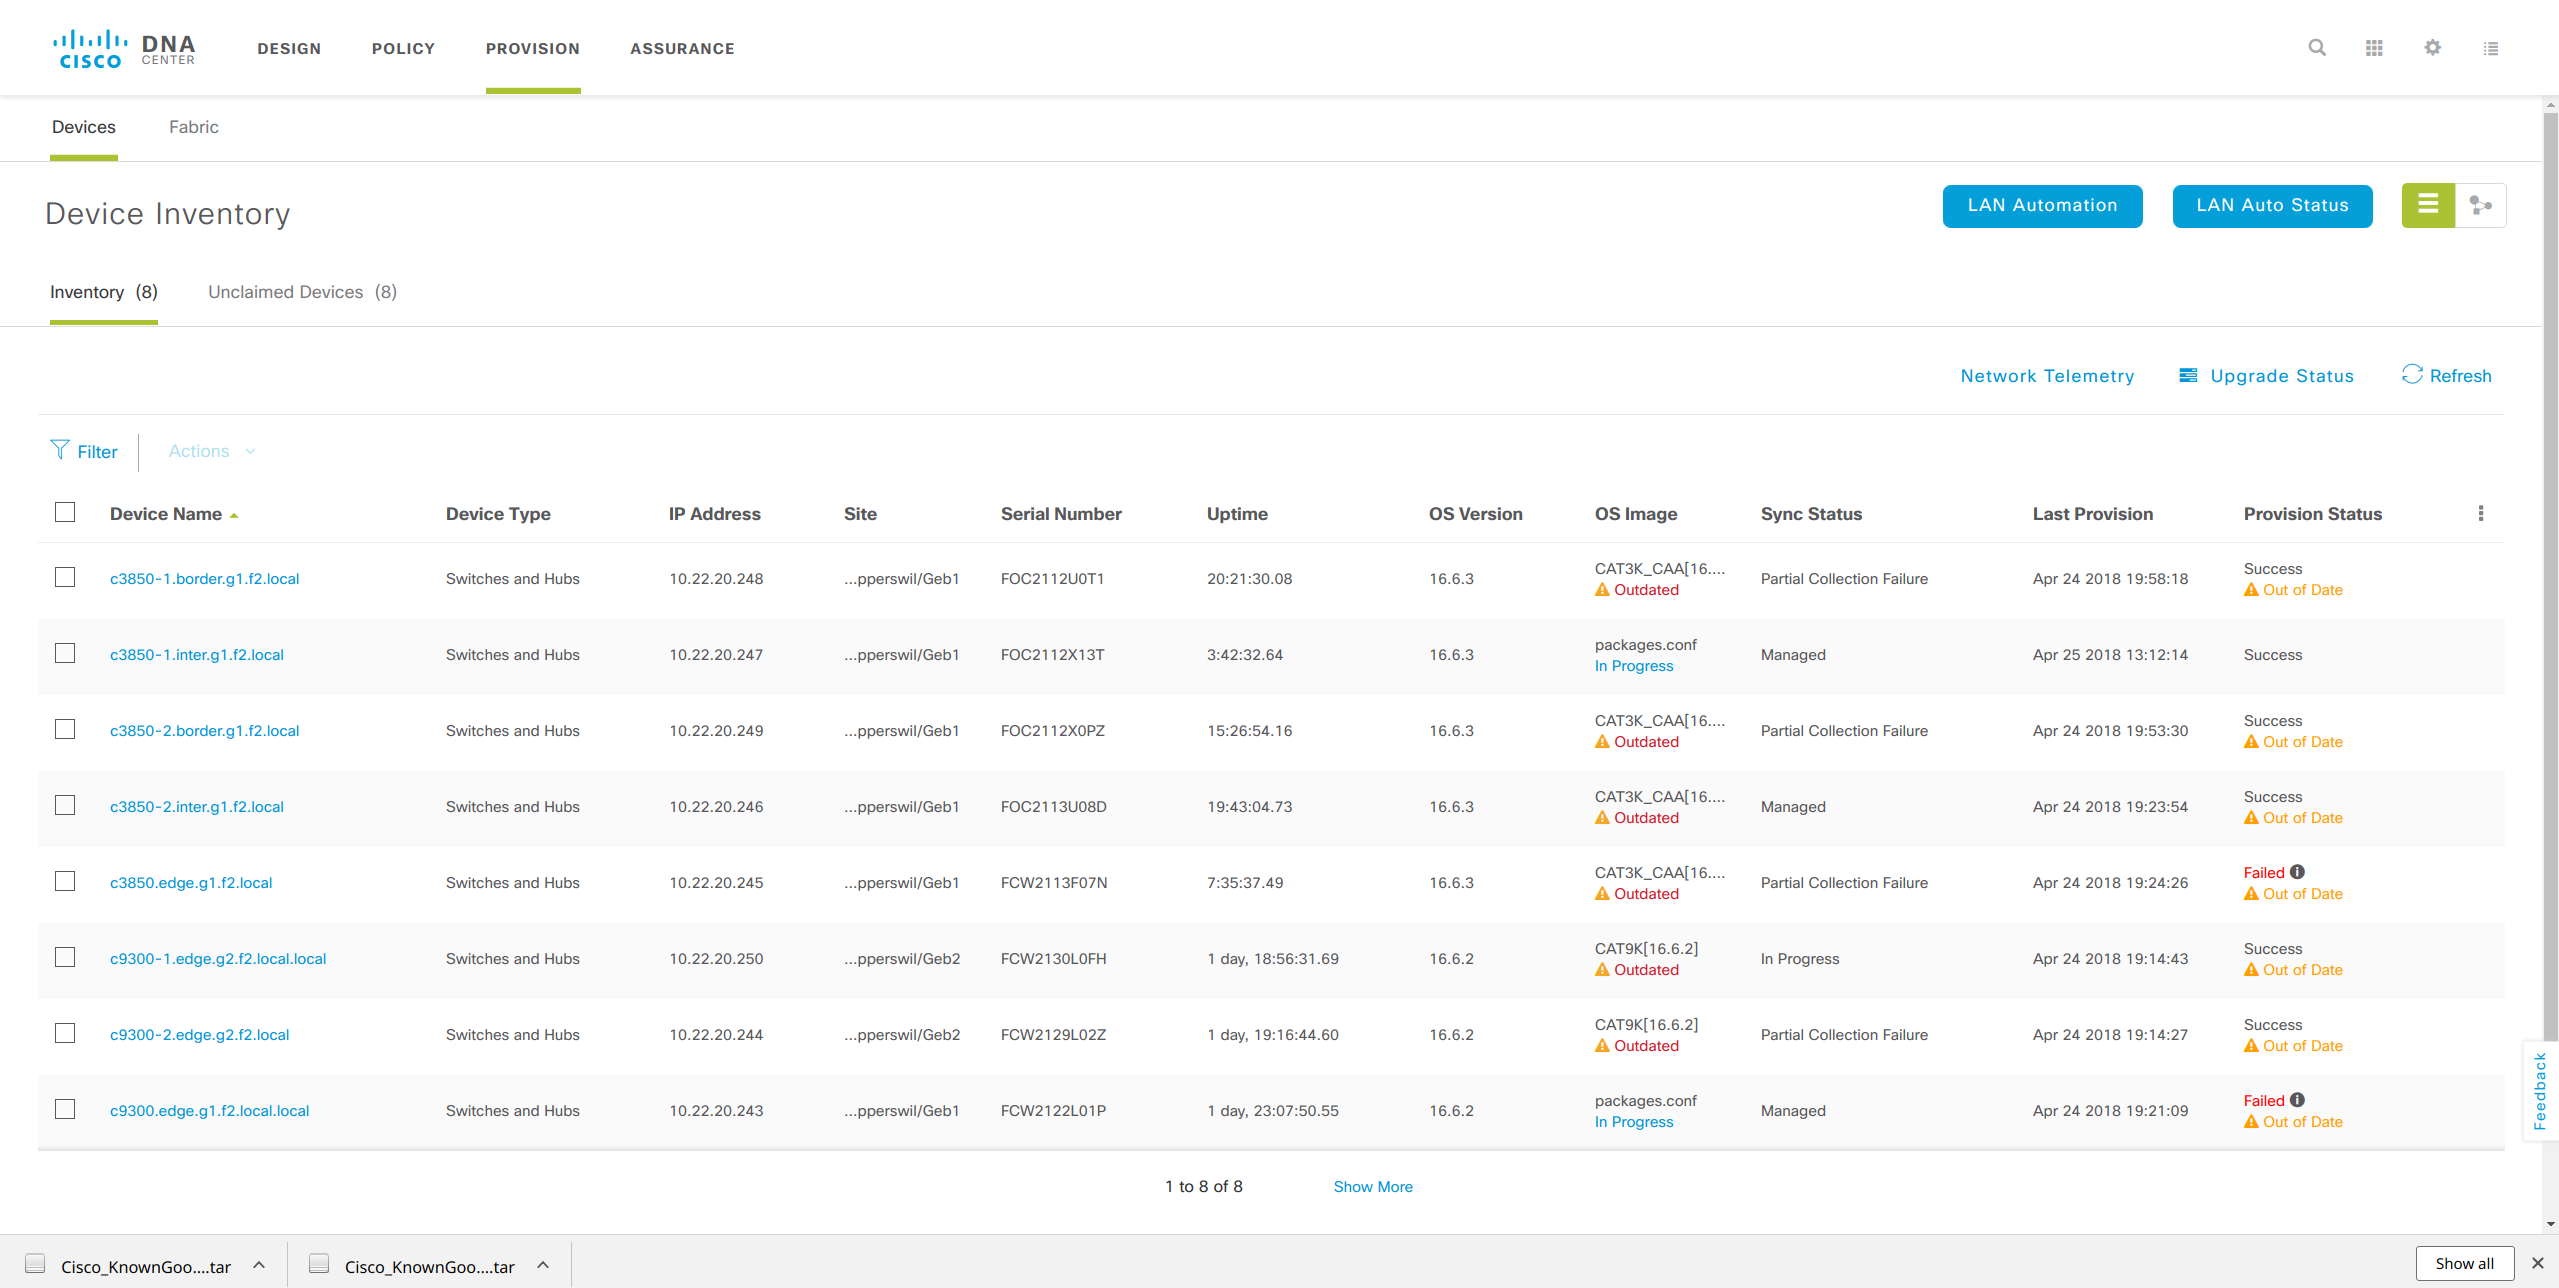
\includegraphics[height=8cm]{img/updates/Selection_070.png}
	\caption{DNA Center Provision - Nach dem manuellen Hinzufügen, muss das OS aktualisiert werden.}
	\label{fig:dna-center-provision-updates}
\end{figure}

Das automatische Softwareupdate hat bei keinem von unseren Switches oder Routern geklappt. Nachfolgend eine kleine Übersicht über die verschiedenen Update Methoden und ausgeführten Versuche.

\begin{tabular}{ | l | l |}
	\hline
	\textbf{Methode} & \textbf{Resultat} \\
	\hline	
	\makecell{DNA Center über HTTP und SFTP} & Fehlgeschlagen (siehe \ref{fig:dna-center-provision-updates-1}) \\
	CLI - HTTPS    & Fehlgeschlagen (siehe \ref{fig:dna-center-provision-updates-2}) \\
	CLI - SCP      & Fehlgeschlagen (siehe \ref{fig:dna-center-provision-updates-3}) \\
	CLI - TFTP     & Erfolgreich (siehe \ref{fig:dna-center-provision-updates-4}) \\	
	\hline
\end{tabular}
\captionof{table}{Softwareupdate - Übersicht Methoden und ausgeführten Versuche}

Beim Versuch die Softwareupdates im DNA-C über HTTP oder SFTP durchzuführen, wurden folgende Fehlermeldungen im DNA-C angezeigt.

\begin{figure}[H]
	\centering
	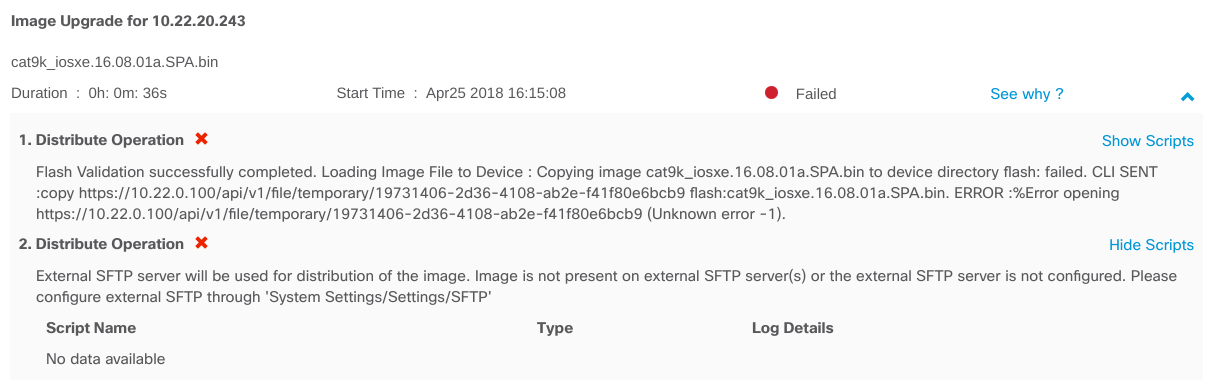
\includegraphics[height=5cm]{img/updates/Selection_071.png}
	\caption{Fehlermeldung Updatevorgang via DNA Center}
	\label{fig:dna-center-provision-updates-1}
\end{figure}

Die Upgrade Prozesse wurden schon beim Herunterladen der einzelnen Images nach unterschiedlicher Dauer immer abgebrochen.

\subsection{Manuelles Softwareupdate via separaten TFTP Server}
Da wie oben beschrieben das automatische Update nicht funktionierte, wurde in einem nächsten Schritt versucht, die Updates manuell auf die Netzwerkgeräte zu installieren. 

\begin{figure}[H]
	\centering
	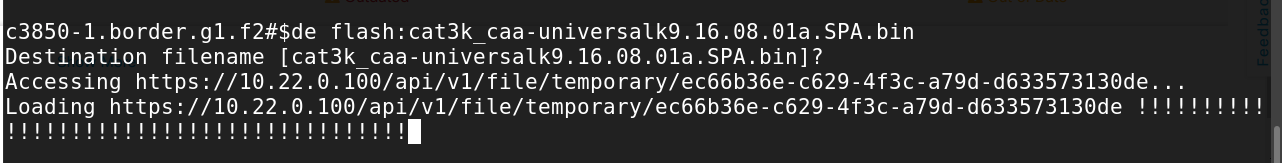
\includegraphics[height=2cm]{img/updates/Selection_082.png}
	\caption{Firmwareupdate Switch via CLI HTTPs}
	\label{fig:dna-center-provision-updates-2}
\end{figure}
Das Herunterladen via HTTPS wurde nach einer gewissen Dauer abgebrochen.

\begin{figure}[H]
	\centering
	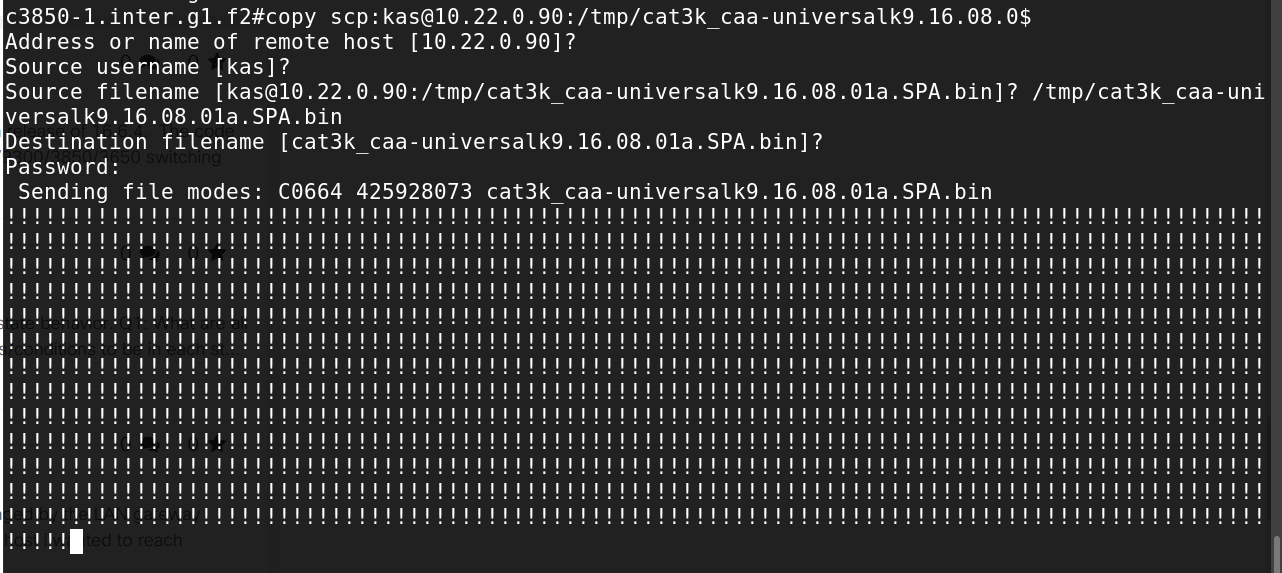
\includegraphics[height=5cm]{img/updates/Selection_108.png}
	\caption{Firmwareupdate Switch via CLI SCP}
	\label{fig:dna-center-provision-updates-3}
\end{figure}
Das Herunterladen via SCP wurde ebenfalls nach einer gewissen Dauer abgebrochen.

\begin{figure}[H]
	\centering
	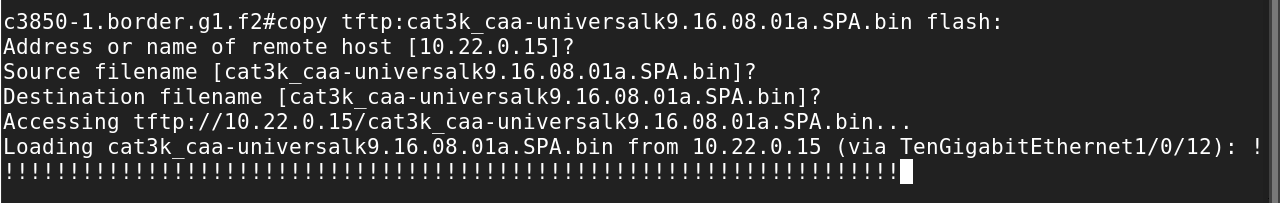
\includegraphics[height=2cm]{img/updates/Selection_111.png}
	\caption{Firmwareupdate Switch via CLI TFTP}
	\label{fig:dna-center-provision-updates-4}
\end{figure}
Der letzte Versuch das Firmwareupdate via TFTP zu installieren war endlich erfolgreich!

\subsection{Lizenzen}
Die Lizenzen bezieht das DNA Center automatisch von den Cisco Server. 
\begin{figure}[H]
	\centering
	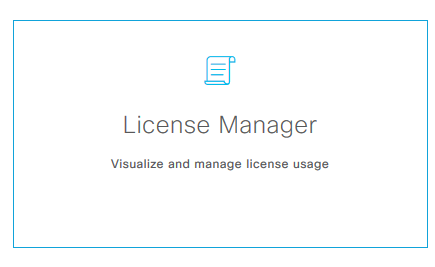
\includegraphics[height=3cm]{img/LicenceManager_001.png}
	\caption{Der Licence Manager ist über das Dashboard erreichbar.}
	\label{fig:dna-center-licence-1}
\end{figure}

\begin{figure}[H]
	\centering
	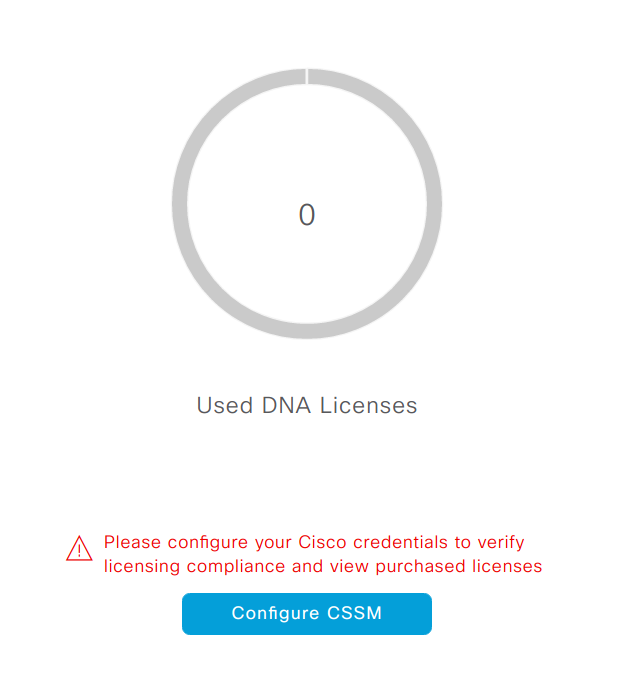
\includegraphics[height=6cm]{img/Selection_006.png}
	\caption{Ohne verlinkten CSSM Account können keine Lizenzen zugewiesen werden.}
	\label{fig:dna-center-licence-3}
\end{figure}

\begin{figure}[H]
	\centering
	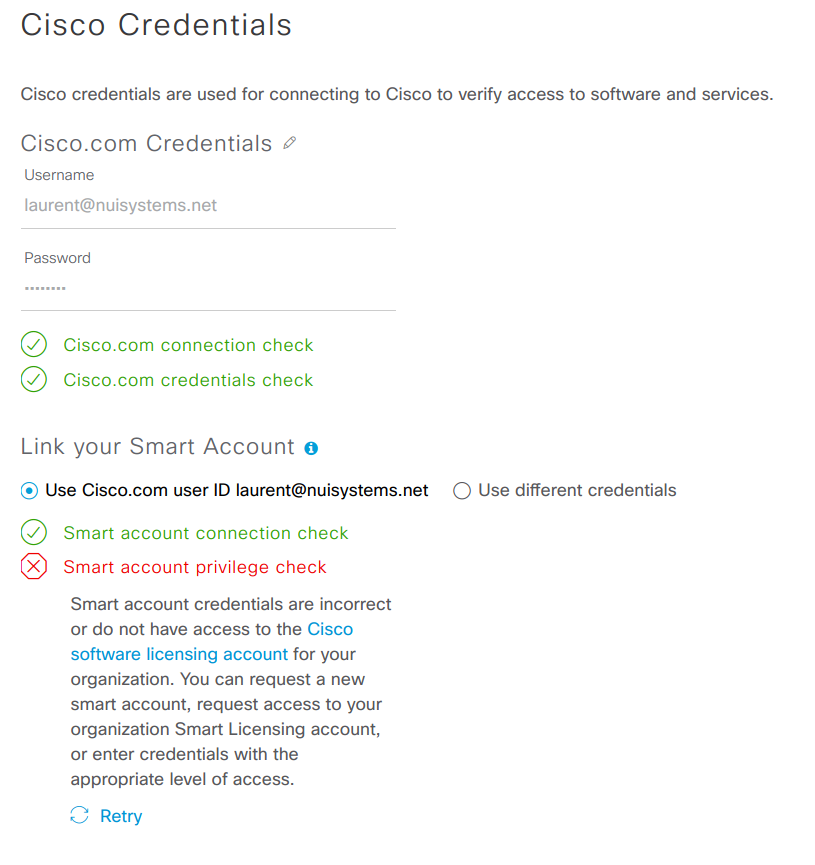
\includegraphics[height=6cm]{img/Selection_008.png}
	\caption{Der im DNA Center hinterlegte Cisco Account muss Zugriff zum entsprechenden Smart Account haben.}
	\label{fig:dna-center-licence-4}
\end{figure}

\begin{figure}[H]
	\centering
	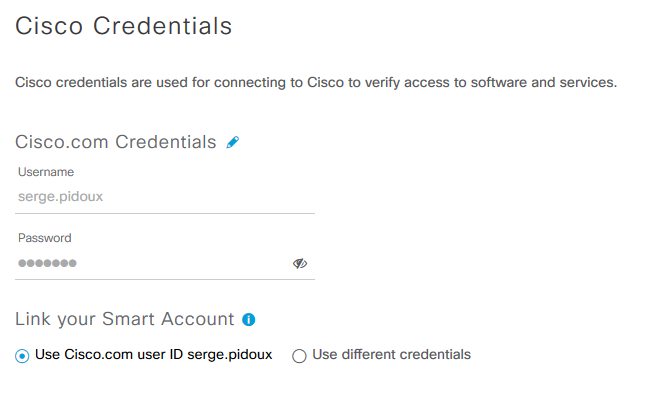
\includegraphics[height=5cm]{img/LicenceManager_002.png}
	\caption{Der korrekt hinterlegte Account}
	\label{fig:dna-center-licence-5}
\end{figure}

\begin{figure}[H]
	\centering
	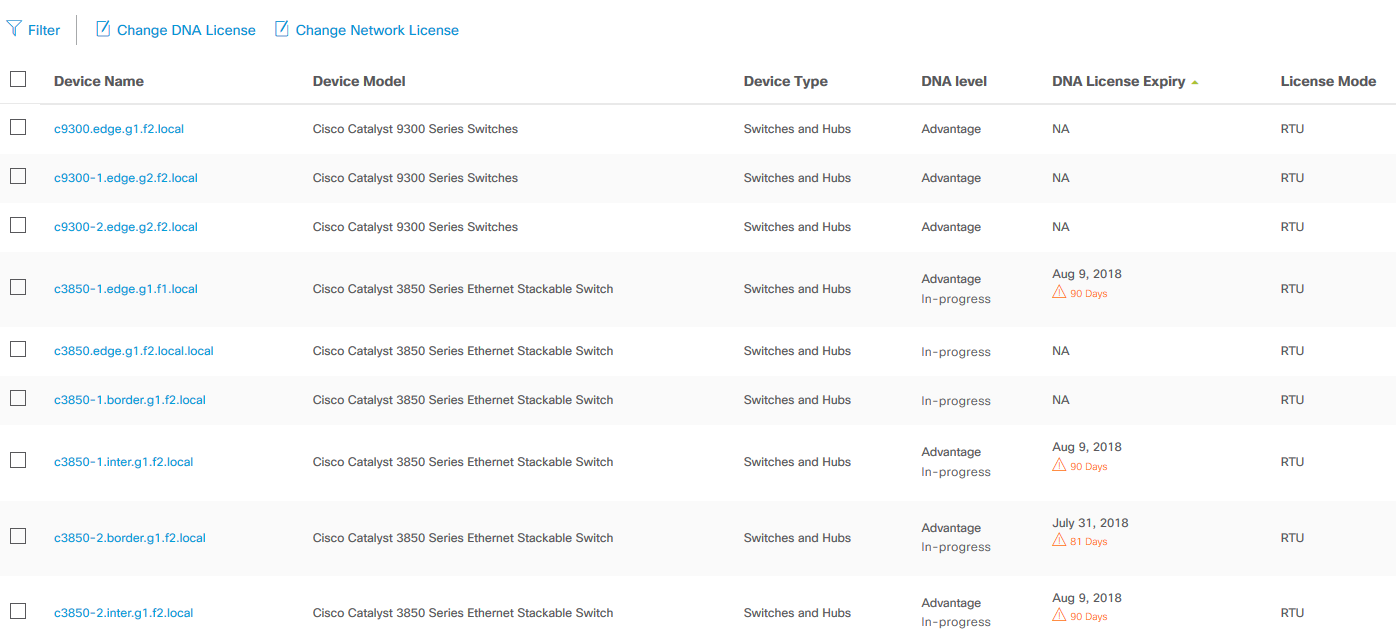
\includegraphics[height=8cm]{img/LicenceManager_003.png}
	\caption{Übersicht über die den Netzwerkkomponenten zugewiesenen Lizenzen}
	\label{fig:dna-center-licence-6}
\end{figure}

\begin{figure}[H]
	\centering
	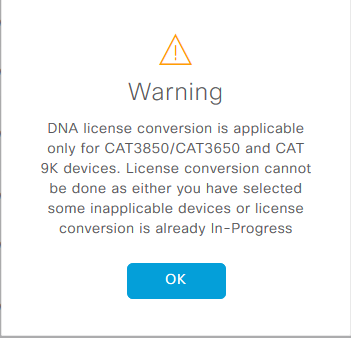
\includegraphics[height=6cm]{img/LicenceManager_004.png}
	\caption{Nicht jedem Gerät kann eine Lizenz zugewiesen werden (Siehe Tabelle)}
	\label{fig:dna-center-licence-7}
\end{figure}

\begin{tabular}{ | c | c | }
	\hline
	\textbf{Geräteserie} & 	\textbf{Lizenzzuweisung möglich} \\
	\hline
	Cisco Catalyst 9300 Series Switches & Ja \\
	Cisco Catalyst 3850 Series Ethernet Stackable Switch & Ja \\
	Cisco 4400 Series Integrated Services Routers & Nein \\
	\hline
\end{tabular}

\subsection{Device Provisioning via DNA Center}
Um den einzelnen Netzwerkgeräten einen Namen und die Basis Konfiguration zu geben, wird im DNA Center unter \textit{Provision $\rightarrow$ Devices} die zu provisionierenden Geräte ausgewählt. Danach wird \textit{Action $\rightarrow$ Provision Device} der Provision Vorgang gestartet.

Dabei wird die komplette Konfiguration, die das DNA Center für ein Device vorsieht auf dem Gerät konfiguriert. Sind Templates für das entsprechende Device konfiguriert worden, werden diese ebenfalls angewendet.
Templates können im Template Editor erstellt und entsprechenden Gerätetypen zugewiesen werden.

\begin{figure}[H]
	\centering
	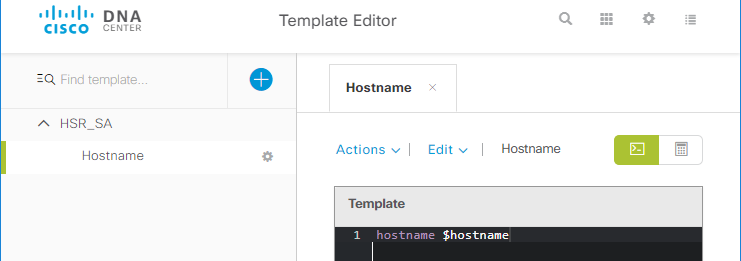
\includegraphics[width=12cm]{img/templateeditor.png}
	\caption{Template Editor}
	\label{fig:Template Editor}
\end{figure}


\subsection{BGP und VRF-Lite}
Automatisierte Weiterleitung externer Verbindungen werden durch Virtual Routing and Forwarding Lite (VRF-Lite) und Border Gateway Protocol Ethernet VPN (BGP-EVPN) unterstützt. Dabei ist uns aufgefallen das die Cisco Catalyst 3850 Series Switche nur eine Lizenz für IP Base installiert haben und BGP sowie VRF-Lite nur in der IP Services Lizenz unterstützt wird. Die genauen Unterschiedene der verschiedenen IOS Software Features sind in untenstehender Grafik ersichtlich\cite{cisco-3850-faq}:

\begin{figure}[H]
	\centering
	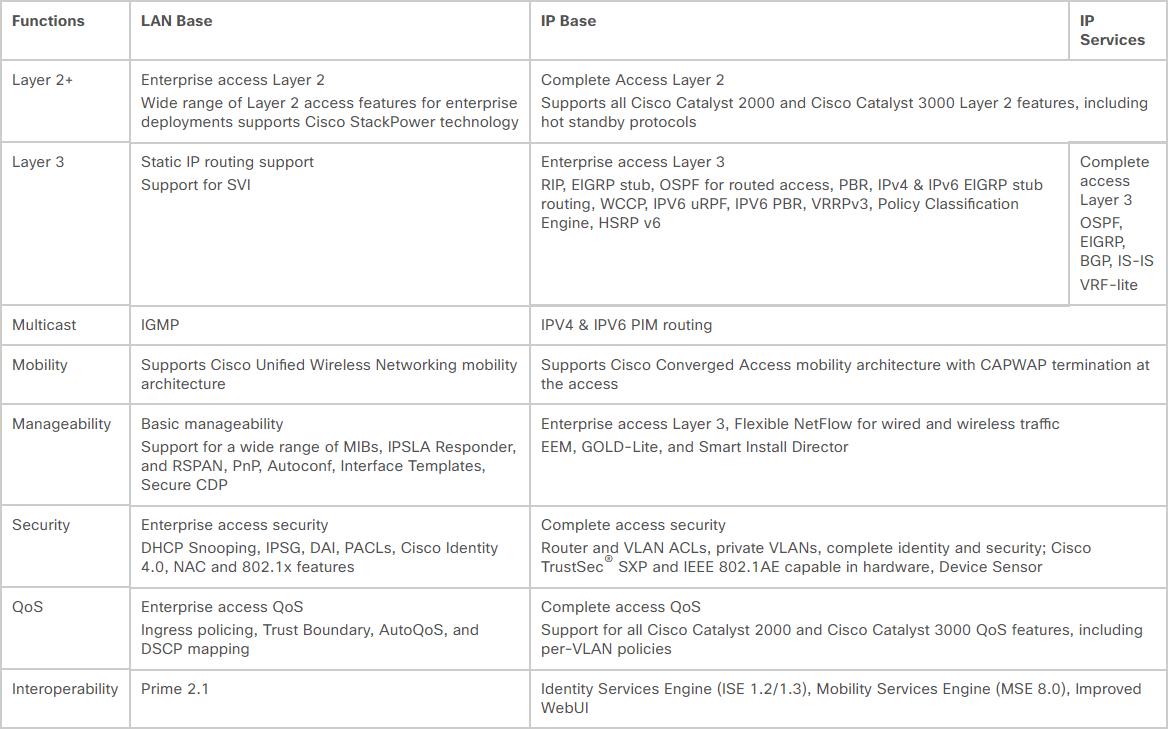
\includegraphics[width=16cm]{img/IPBaseServices.png}
	\caption{IP Base and Services}
	\label{fig:IP Base and Services}
\end{figure}

Über die CLI konnten konnten wir eine IP Services Evaluation Lizenz für 90 Tage aktivieren.

\begin{lstlisting}[language=bash]
sh license right-to-use activate ipservices all accepptEULA
reload
show license right-to-use
\end{lstlisting}

\subsection{Fabric Konfigurieren}
Nach der manuellen Konfiguration des Underlays, dem hinzufügen der Geräte, dem Update und dem Provisionieren, konnten wir endlich die Fabric konfigurieren. 

Erreichbar ist das unter \textit{Provision $\rightarrow$ Fabric}. Nachfolgend wird die Fabric des entsprechenden Standortes ausgewählt.

Den einzelnen Netzwerkgeräten werden nun mit Rechtsklick folgende Rollen zugeteilt:
\begin{itemize}
	\item Border
	\item Border + CP (Control Plane)
	\item Edge
\end{itemize}

Nachdem alle Geräte der entsprechenden Fabric zugeteilt worden sind, kann die Konfiguration gespeichert werden und wird auf die Geräte geschrieben. 

\begin{figure}[H]
	\centering
	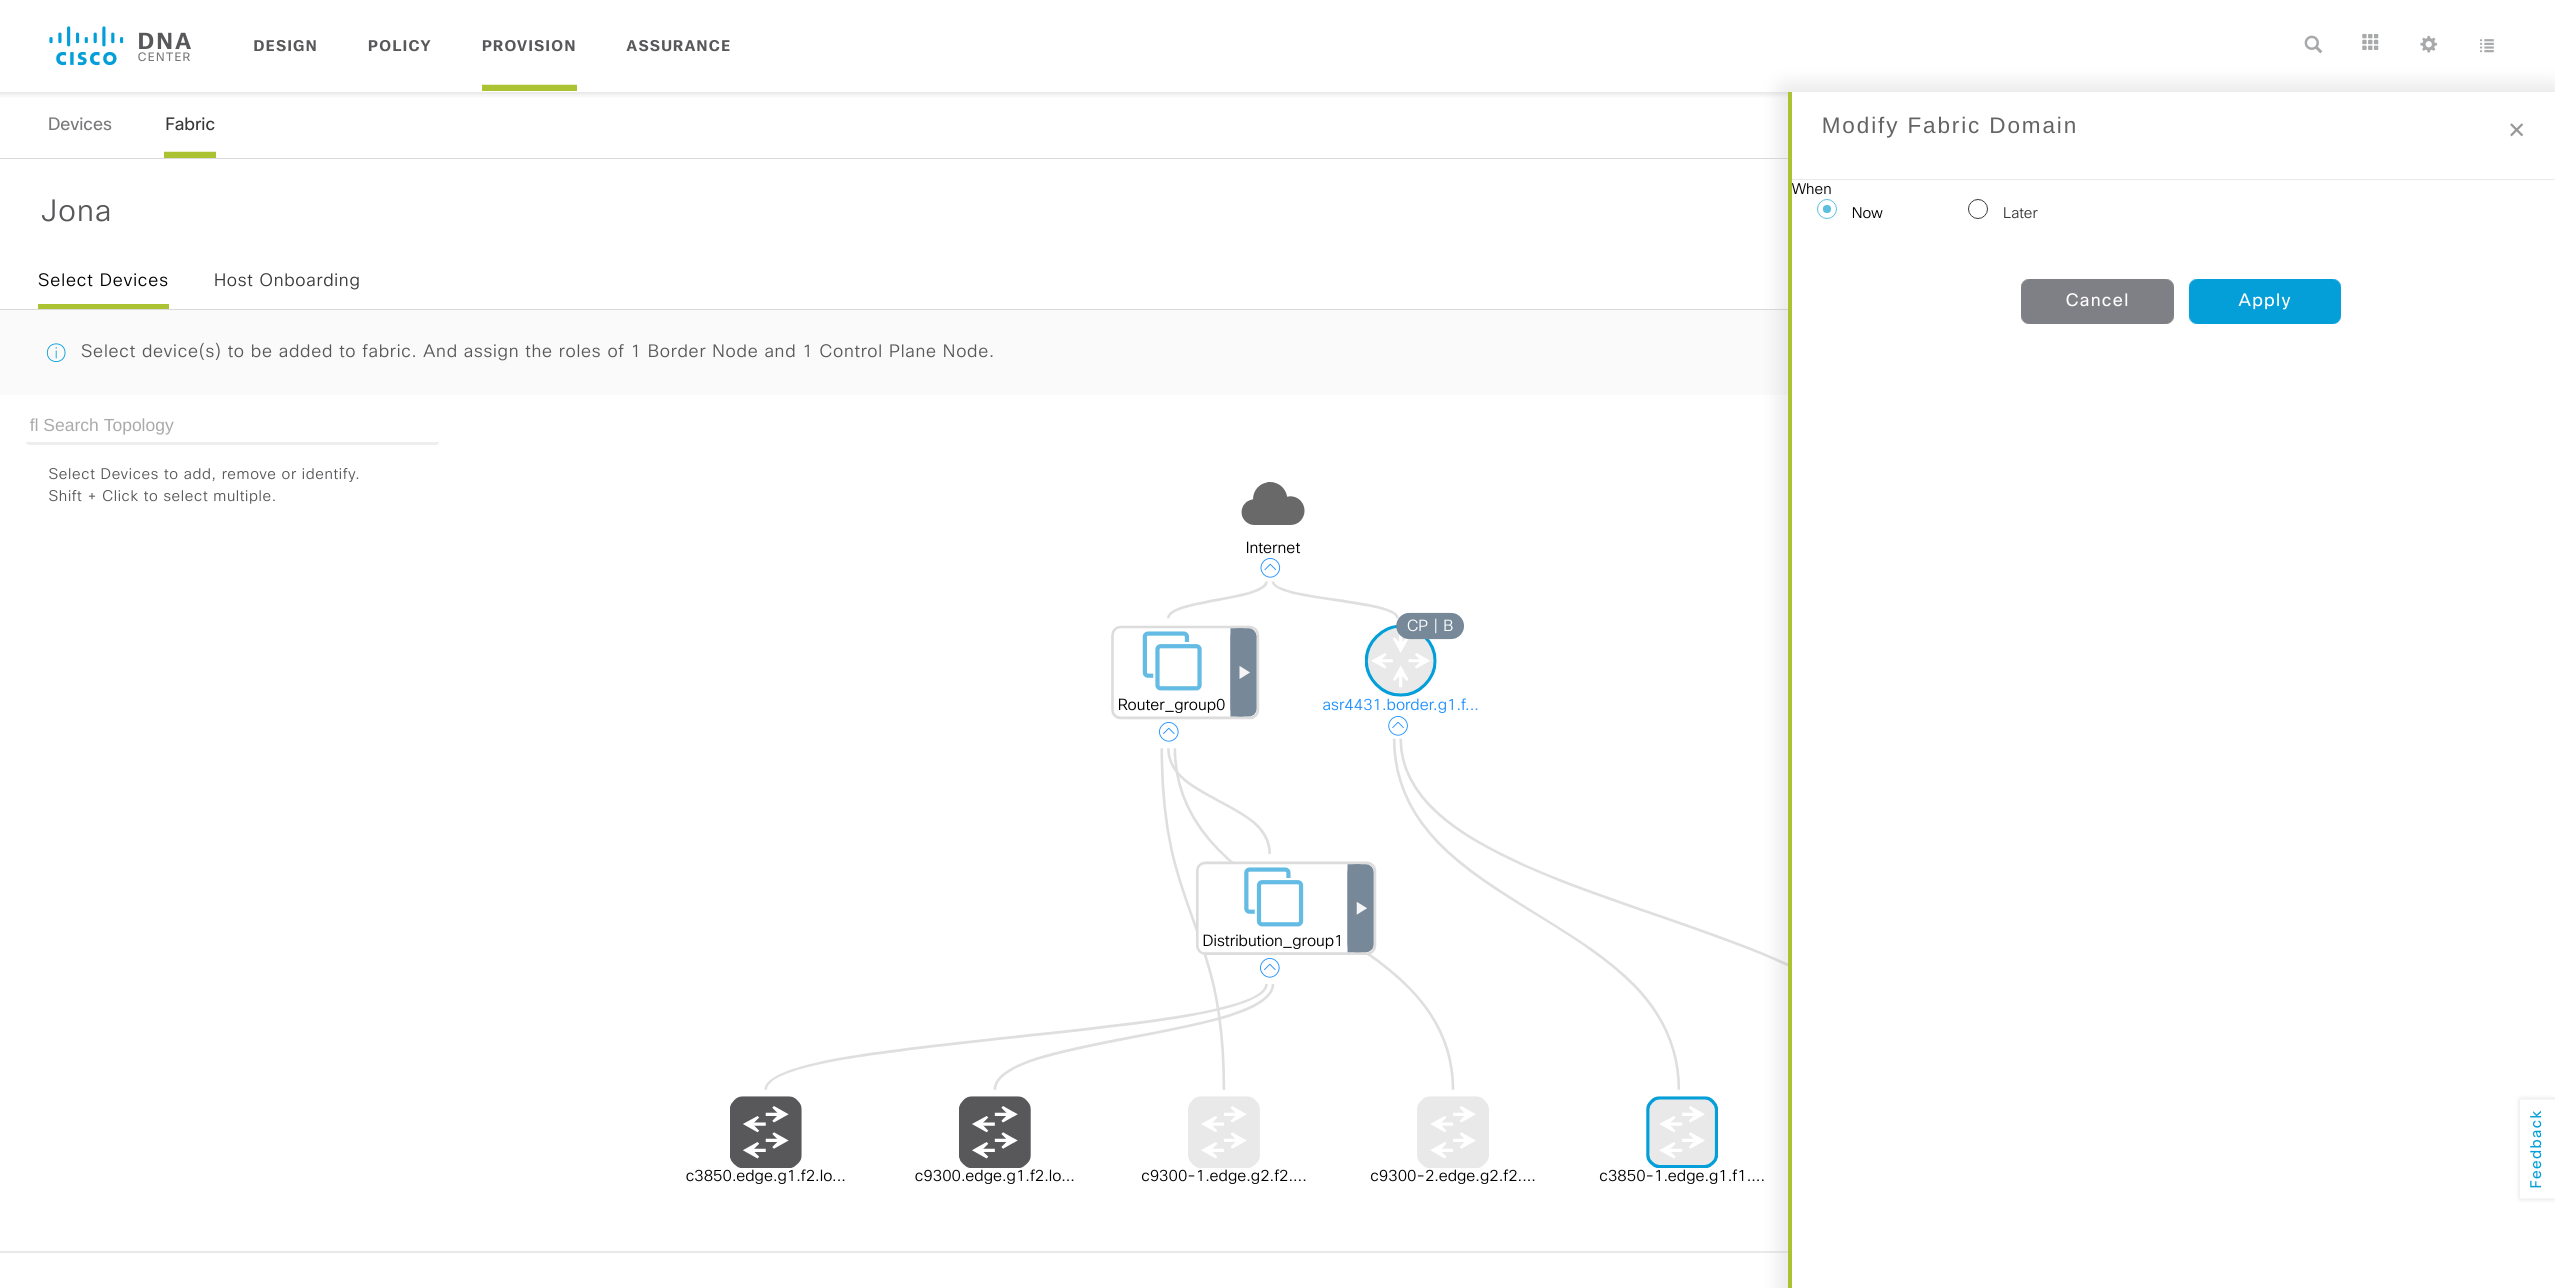
\includegraphics[width=16cm]{img/dna-center-fabric-1.png}
	\caption{DNA Center Provision - Fabric - Nach der Zuteilung wird die Konfiguration auf die Geräte geschrieben.}
	\label{fig:IP Base and Services}
\end{figure}


\begin{tabular}{| l | l | l | l | l |}
	\hline
	\textbf{Darstellung} & \makecell{\textbf{Teil der}\\ \textbf{Fabric}} & \makecell{\textbf{Änderung}\\ \textbf{ausstehend}} & \textbf{Provisioniert} & \textbf{Bemerkung} \\
	\hline
	Grau & Ja & Nein & Nein & \\
	Schwarz & Nein & Nein & Nein & \\
	Grau mit blauem Rand & Ja & Ja & Nein & \\
	Blau & Ja & Nein & Ja & \\
	Umrandung mit Pfeil & - & - & - & Gruppierte Geräte\\	
	\hline
\end{tabular}
\captionof{table}{DNA Center Provision - Fabric - Darstellung}

\subsection{Policies definieren}
Damit die Fabric Konfiguriert werden kann, müssen folgende Bedienungen erfüllt sein:


\subsection{Cisco ISE Verknüpfen und Gruppen anlegen}
TBA

\subsection{Ping zwischen zwei Clients}

\subsection{DNA Center Reset}
Da nach einigen Versuchen weder ein funktionsfähiges Under- noch Overlay Netzwerk vorhanden war, hatten wir uns entschieden das DNA Center neu zu Konfigurieren.

\begin{lstlisting}[language=bash]
$ maglev-config-wizard #DO NOT EXECUTE THIS COMMAND
\end{lstlisting}

Als folge dieses Befehls, nachdem alle Parameter eingegeben wurden, kam die folgende Meldung:

\begin{figure}[H]
	\centering
	\includegraphics[height=10cm]{img/dna-center-reset-fail-1.png}
	\caption{DNA Center - maglev-config-wizard - Fehlermeldung}
	\label{fig:dna-center-reset-1}
\end{figure}

Nach einem Neustart der Appliance kam die folgende Meldung und das System bootete nicht mehr. 
\begin{figure}[H]
	\centering
	\includegraphics[height=1cm]{img/dna-center-reset-fail-2.png}
	\caption{DNA Center - Boot Fehlermeldung}
	\label{fig:dna-center-reset-2}
\end{figure}

In der Anleitung wird dieser Befehl so nicht erwähnt. Bei einem früheren Versuch diesen Befehl auszuführen, um den NTP Server zu ändern, führte es jedoch nicht zu diesem Fehler. 

\paragraph{Neuinstallation}
In folge war es notwendig die Cisco DNA Center Appliance neu zu installieren. 

\begin{figure}[H]
	\centering
	\includegraphics[height=2cm]{img/dna-center-reset-iso.png}
	\caption{DNA Center - Neuinstallation - Installations ISO wird auf USB Drive kopiert}
	\label{fig:dna-center-iso-1}
\end{figure}

Das USB Drive wird direkt in die Appliance gesteckt und gebootet. Der weitere Installationsprozess sieht aus wie im Abschnitt \ref{DNACenterSetup_Installation} gezeigt. 

\alertwarningbox{
	Nach der Neuinstallation sind alle Daten und die Konfiguration gelöscht. Eine Option die Konfiguration beizubehalten gibt es nicht.
}

\subsection{Zweiter Versuch}
Im ersten Versuch haben wir die LAN Automation übersprungen. Das stellt jedoch einer der wichtigen Features des DNA Centers dar. Mit der Unterstützung von Patrick Mosimann sind wir alles Schritt für Schritt durchgegangen. 

\subsection{DNA Center Netzwerk Design}
Wie im ersten Teil

\subsection{Downgrade aller Netzwerkkomponenten}
Nach Absprache mit dem Experten von Cisco, mussten alle Switch und Router auf eine spezifische Version zurückgesetzt werden.

Neue Version: 16.6.3

\subsection{ISE reset}
Um die Störungen durch alte Konfigurationen zu vermeiden, wurde das Cisco ISE Center ebenfalls zurückgesetzt. Dies kann einfach mittels eines Befehls durchgeführt werden.

\begin{lstlisting}[language=bash]
ISE/admin# applicaiton reset-config ise
\end{lstlisting}

\begin{figure}[H]
	\centering
	\includegraphics[height=6cm]{img/secondtry/s2t-cisco-ise-reset.png}
	\caption{Cisco ISE Reset}
	\label{fig:dna-ise-reset-1}
\end{figure}

\subsection{Credentials korrekt hinterlegen}
TBA

\subsection{ISE Integration}
TBA

\subsection{Fabric Border - Seeddevice}
Bevor die LAN Automation gestartet werden kann, müssen folgende Bedinungen erfüllt sein:
\begin{itemize}
	\item Aktives SSH
	\item IP Konnektivität
\end{itemize}

\subsubsection{Verbindung zwischen Legacy Router und Border Switch}
Um eine Verbindung über den Legacy Router zu ermöglichen, musste ein VLAN angelegt werden.

\paragraph{Konfiguration auf Border Switch}
\begin{lstlisting}[language=bash]
# interace XY
# switchport trunk native vlan 100
# interface vlan 100
# ip adress 10.22.31.1 255.255.255.252
# exit
# ip route 10.22.0.0 255.255.255.0 10.22.31.0
\end{lstlisting}

\paragraph{Konfiguration auf Legacy Router}
\begin{lstlisting}[language=bash]
# interface GigabitEthernet0/0/1.100
# encapsulation dot1Q 100
# ip address 10.22.31.2 255.255.255.252
\end{lstlisting}

\subsection{Border BGP}
\begin{lstlisting}[language=bash]
router bgp 10
bgp log-neighbor-changes
neighbor 10.22.11.1 remote-as 30
address-family ipv4
redistribute connected
neighbor 10.22.11.1 activate
exit-address-family
\end{lstlisting}

\subsection{Trustpool}
Zuvor ist das Zertifikat des DNA Centers ersetzt worden. Den gemäss \cite{cisco-dna-appliance-installation-guide-release-1-1} ist es für den ISE Version 2.4 erforderlich, dass die IP Adresse des DNA Centers im Zertifikat hinterlegt worden. Da die Version 2.4 sowieso nicht mit dem DNA Center Version 1.1.5 kompatibel ist, musste der ISE in der Version 2.3 neu installiert werden. Dies hat diese spezielle Anforderung an das Zertifikat nicht. Da das benutzerdefinierte Zertifikat die LAN Automation behinderte. Stellten wir das alte Zertifikat wieder her.

Mit dem folgenden Befehl konnte das ursprüngliche Zertifikat lokal heruntergeladen.

\begin{lstlisting}[language=bash]
scp -r -P 2222 maglev@10.22.0.100:/etc/maglev/.pki .
\end{lstlisting}

In DNA Center unter \textit{System Settings $\rightarrow$ Settings $\rightarrow$ Certificate} wurde das gebergte Zertifikat eingespielt. 

\begin{figure}[H]
	\centering
	\includegraphics[height=8cm]{img/secondtry/dna-center-replace-certificate.png}
	\caption{Cisco DNA Center - Zertifikat ändern}
	\label{fig:dna-zertificate-1}
\end{figure}


\subsection{Netzwork Discovery - LAN Automation - Zweiter Versuch}
\label{Netzwork Discovery - LAN Automation - Zweiter Versuch}
Die Netzwerk Discovery braucht mehr Eingriffe als erwartet. Im ersten Schritt haben wir versucht alle Geräte auf der Seite Rapperswil einzuspielen. Dies hat nicht geklappt. Das PNP schlägt fehl. Deshalb sind wir wie folgt vorgegangen:
\begin{enumerate}
	\item Ein Netzwerkgerät im \textit{Initial Config Dialog} Zustand lassen. (Siehe: \ref{fig:cisco-switch-initial-config})
	\item LAN Automation durchführen. (Siehe \ref{fig:dna-lan-automation-dialog})
	\item Vorgang wiederholen, bis alle Geräte hinzugefügt sind. 
\end{enumerate}

\begin{figure}[H]
	\centering
	\includegraphics[height=0.5cm]{img/secondtry/cisco-switch-initial-config.png}
	\caption{Cisco Switch - Initial Config - Versucht DHCP und PNP zu machen, solange der Dialog aktiv ist.}
	\label{fig:cisco-switch-initial-config}
\end{figure}

\begin{figure}[H]
	\centering
	\includegraphics[height=7cm]{img/secondtry/dna-lan-automation-dialog.png}
	\caption{Cisco Switch - DNA LAN Automation}
	\label{fig:dna-lan-automation-dialog}
\end{figure}

\alertwarningbox{
	Die LAN Automation funktionierte nur mit den Standard Zertifikaten. 
}

\subsection{Broken ISIS - Gründe}
TBA

\subsection{Provisioning}

\subsubsection{Script Template}
\label{Script Template}
Damit der Hostname der Switches und Router via Provisioning gesetzt werden kann, muss ein Template angelegt werden.

Über das Hauptmenü \textit{Tools $\rightarrow$ Template Editor} kann mit \textit{Add (Pluszeichen) $\rightarrow$ Create Project} ein neues Projekt anlegt werden. (Siehe: \ref{fig:dna-center-template-editor-add-project})

\begin{figure}[H]
	\centering
	\includegraphics[height=7cm]{img/secondtry/dna-center-template-editor-add-project.png}
	\caption{Cisco DNA Center - Templateeditor - Add Project}
	\label{fig:dna-center-template-editor-add-project}
\end{figure}

Weiter kann mit \textit{Add (Pluszeichen) $\rightarrow$ Add Template} ein neues leeres File angelegt werden. (Siehe \ref{fig:dna-center-template-editor-add-template})

\begin{figure}[H]
	\centering
	\includegraphics[height=7cm]{img/secondtry/dna-center-template-editor-add-template.png}
	\caption{Cisco DNA Center - Templateeditor - Add Template}
	\label{fig:dna-center-template-editor-add-template}
\end{figure}

Wie in Abbilung \ref{fig:dna-center-template-editor-add-template} sind folgende Einstellungen festzulegen:
\begin{itemize}
	\item Name des Templates
	\item Zugehörige Projekt
	\item Beschreinbung
	\item Tags
	\item Für welche \textit{Device Types} das Template verwendet werden soll.
\end{itemize}

\begin{figure}[H]
	\centering
	\includegraphics[height=7cm]{img/secondtry/dna-center-template-editor-edit.png}
	\caption{Cisco DNA Center - Templateeditor - Template um den Hostname bei der Provisionierung zu setzen.}
	\label{fig:dna-center-template-editor-edit}
\end{figure}

\subsubsection{Network Profile anlegen}
Unter \textit{Design $\rightarrow$ Network Profiles $\rightarrow$ Add Profile} kann ein neues Profil angelegt werden. Dieses Profil wird während des Provisionierungsvorgang verwendet. 

\begin{figure}[H]
	\centering
	\includegraphics[height=4cm]{img/secondtry/dna-center-network-profile-new.png}
	\caption{Cisco DNA Center - Network Profile - New Profile}
	\label{fig:dna-center-network-profile-new}
\end{figure}

Weiter wird festgelegt für welche \textit{Sites} das Netzwerkprofil verwendet werden soll. 

\begin{figure}[H]
	\centering
	\includegraphics[height=5cm]{img/secondtry/dna-center-network-profile-assign-sites.png}
	\caption{Cisco DNA Center - Network Profile - Assign Sites}
	\label{fig:dna-center-network-profile-assign-sites}
\end{figure}

\subsubsection{Claimed Netzwerkgeräte Provisionierung}

Die Provisionierung gestaltet sich im Normalfall sehr einfach. Im Modul \textit{Provision $\rightarrow$ Devices $\rightarrow$ Inventory}

Das zu provisionierende Gerät wird in der Liste ausgewählt. Über \textit{Action $\rightarrow$ Provision} wird die Provision gestartet. 

\begin{figure}[H]
	\centering
	\includegraphics[height=5cm]{img/secondtry/dna-center-provision-device.png}
	\caption{Cisco DNA Center - Netzwerkgerät konfigurieren}
	\label{fig:dna-center-provision-device}
\end{figure}

Im ersten Schritt (Siehe: \ref{fig:dna-center-provision-step1}) wird die entsprechende \textit{Site} ausgewählt. 

\begin{figure}[H]
	\centering
	\includegraphics[height=3cm]{img/secondtry/dna-center-provision-step1.png}
	\caption{Cisco DNA Center - Provision Step 1}
	\label{fig:dna-center-provision-step1}
\end{figure}

Im zweiten Schritt gibt es keine wählbaren Optionen. 

Im dritten Schritt kann das in im Abschnitt \cite{Script Template} ausgewählt werden. Die offnen Variablen (im Falle \ref{fig:dna-center-provision-step3}) werden hier hinterlegt. 

\begin{figure}[H]
	\centering
	\includegraphics[height=4cm]{img/secondtry/dna-center-provision-step3.png}
	\caption{Cisco DNA Center - Provision Step 3}
	\label{fig:dna-center-provision-step3}
\end{figure}

Im letzte Schritt erscheint eine Übersicht. Mit einem Klick auf \textit{Deploy} wird der Script provisioniert. Die dabei automatisch ausgeführten Befehle durch das DNA Center sind in Listing \ref{lst:commands-executed-during-provision} ersichtlich.


\begin{lstlisting}[caption={Befehle automatisch ausgeführt durch das DNA Center während der Provisionierung},label={lst:commands-executed-during-provision},language=bash]
enable
no ip domain-lookup 
ip access-list extended ACL_WEBAUTH_REDIRECT
180 permit tcp any any eq www 
190 permit tcp any any eq 443 
200 permit tcp any any eq 8443 
210 permit udp any any eq domain 
220 permit udp any eq bootpc  any eq bootps 
170 deny ip any host 10.22.0.22
exit 
ip tacacs source-interface Loopback0 
ip radius source-interface Loopback0 
aaa new-model 
ip radius source-interface Loopback 0
exit 
aaa group server radius dnac-network-radius-group
server name dnac-radius_10.22.0.22
ip radius source-interface Loopback 0
exit 
aaa accounting dot1x default start-stop group dnac-client-radius-group
aaa accounting update newinfo periodic 600
aaa accounting exec default start-stop group dnac-network-radius-group
aaa authorization network dnac-cts-list group dnac-client-radius-group
aaa authorization exec VTY_author group dnac-network-radius-group local if-authenticated 
aaa authorization exec VTY_author group dnac-network-radius-group local 
aaa authentication login default local 
aaa authentication dot1x default group dnac-client-radius-group
aaa authentication login VTY_authen group dnac-network-radius-group local 
dot1x system-auth-control 
radius server dnac-radius_10.22.0.22
address ipv4 10.22.0.22 auth-port 1812 acct-port 1813
pac key *
retransmit 1
radius-server deadtime 30
radius-server attribute 25 access-request include 
radius-server attribute 8 include-in-access-req 
radius-server attribute 6 on-for-login-auth 
radius-server attribute 6 support-multiple 
cts authorization list dnac-cts-list
line vty 0 97
login authentication VTY_authen
authorization exec VTY_author
transport input all 
enable
enable
banner motd #\"Welcome to our SA Lab!\"#
hostname c9300-2.edge.g2.f2
enable
enable
enable
enable
enable
enable
enable
\end{lstlisting}

\subsection{Fabric}

\subsubsection{Device Role zuordnen}

\subsubsection{Add to Fabric}
Screenshots und vorgehen. 

\begin{lstlisting}[caption={Befehle automatisch ausgeführt durch das DNA Center während dem hinzufügen zur Fabric},label={lst:commands-executed-during-add-to-fabric},language=bash]
!exec: enable
ip dhcp snooping 
cts role-based enforcement 
vrf definition DEFAULT_VN
address-family ipv4 
vlan 4000
name VOICE_VLAN
exit 
vlan 3999
name CRITICAL_VLAN
exit 
interface GigabitEthernet1/0/3 
no load-interval 
no spanning-tree portfast 
no switchport trunk native vlan 
switchport 
switchport mode dynamic auto 
switchport access vlan 1
exit 
interface GigabitEthernet1/0/4 
no load-interval 
no switchport trunk native vlan 
switchport 
switchport mode dynamic auto 
switchport access vlan 1
exit 
interface GigabitEthernet1/0/7 
no load-interval 
no spanning-tree portfast 
no switchport trunk native vlan 
switchport 
no switchport trunk native vlan 
switchport 
switchport mode dynamic auto 
switchport access vlan 1
exit 
interface GigabitEthernet1/0/10 
no load-interval 
no spanning-tree portfast 
no switchport trunk native vlan 
switchport 
interface GigabitEthernet1/0/12 
no load-interval 
no spanning-tree portfast 
no switchport trunk native vlan 
switchport 
switchport mode dynamic auto 
switchport access vlan 1
exit 
interface GigabitEthernet1/0/13 
no load-interval 
no switchport trunk native vlan 
switchport 
switchport mode dynamic auto 
switchport access vlan 1
exit 
interface GigabitEthernet1/0/15 
no load-interval 
no spanning-tree portfast 
no switchport trunk native vlan 
switchport 
switchport 
switchport mode dynamic auto 
switchport access vlan 1
exit 
interface GigabitEthernet1/0/18 
no load-interval 
no spanning-tree portfast 
no switchport trunk native vlan 
switchport 
switchport mode dynamic auto 
switchport access vlan 1
exit 
interface GigabitEthernet1/0/21 
no load-interval 
no spanning-tree portfast 
no switchport trunk native vlan 
switchport 
switchport mode dynamic auto 
switchport access vlan 1
exit 
switchport access vlan 1
exit 
router lisp 
ipv4 source-locator Loopback0 
locator-set rloc_def9f1a7-9572-4e74-afaf-44215f0fbbde
IPv4-interface Loopback0 priority 10 weight 10
exit 
locator-table default 
locator default-set rloc_def9f1a7-9572-4e74-afaf-44215f0fbbde
service ipv4 
etr map-server 10.22.10.67 proxy-reply 
etr 
sgt 
use-petr 10.22.10.67
use-petr 10.22.30.1
exit 
service ethernet 
database-mapping limit dynamic 5000
map-cache-limit 25000
itr map-resolver 10.22.30.1
ipv4 locator reachability exclude-default 
ip dhcp relay information option 
banner motd #\"Welcome to our SA Lab!\"#
ip sla 1
icmp-echo 10.22.0.22 source-ip 10.22.10.65
frequency 60
threshold 3
timeout 5000
ip sla schedule 1  life forever start-time now 
banner motd #\"Welcome to our SA Lab!\"#
ip sla 2
icmp-echo 10.22.10.67 source-ip 10.22.10.65
frequency 60
threshold 3
timeout 5000
ip sla schedule 2  life forever start-time now 
banner motd #\"Welcome to our SA Lab!\"#
ip sla 3
icmp-echo 10.22.30.1 source-ip 10.22.10.65
frequency 60
threshold 3
timeout 5000
ip sla schedule 3  life forever start-time now 
banner motd #\"Welcome to our SA Lab!\"#
\end{lstlisting}

\subsection{LAN Automation - Dritter Versuch}
Da das DNA Center nur ein Teil der Links zwischen den Switches konfiguriert hat, entschieden wir uns diese nochmals neu durchzuführen. Ausser dem Seed Device haben wir alle Devices gelöscht. Danach starteten wir die LAN Automation nochmals (siehe Abschnitt \ref{Netzwork Discovery - LAN Automation - Zweiter Versuch}).

\begin{enumerate}
	\item LAN Automation starten
	\item Switches und Router so lange neu Booten bis PNP erfolgreich ist.
	\item LAN Automation stoppen
\end{enumerate}

\paragraph{Resultat}
Alle Devices und Links wurden erfolgreich konfiguriert. Das "Schritt-für-Schritt" hinzufügen vom vorherigen Versuch funktioniert nicht. Möglicherweise ist das spätere automatische Hinzufügen von Netzwerkgeräten zu einem Underlay nicht möglich. 

\subsection{Lizenzen auf Netzwerkgeräten nach Underlay Automation}
Geräte haben nicht mer EVAL sondern plötzlich Permanent Lizenzen

\subsection{Ping to Clients}

\subsection{Host Onboarding}

Infoblox vorgehen bei neuem Netzwerk!!!

\subsubsection{Authentifizierungsmethoden}

\begin{tabular}{ | m{8cm} | m{8cm} | }
	\hline
	\textbf{Typ} & 	\textbf{Beschreibung} \\
	\hline
	Closed Authentication & Based on 802.1X. Authentication MUST succeed prior to network access. Requires networks with complete 802.1x support. \\
	Open Authentication & Based on 802.1x. Temporary access is granted (e.g. PXE, DHCP) prior to authentication. Optimal for networks with limited 802.1x support. \\
	Easy Connect & Based on LDAP combined with MAC Address Bypass (MAB). Optimal for networks using Active Directory (AD) authentication. \\
	No Authentication & Optimal for networks that do not support authentication or require static configuration. \\
	\hline

\end{tabular}
\caption[Erklärung der Host Onboardning Authentifizierungsmethoden]{Erklärung der Host Onboardning Authentifizierungsmethoden.\cite{ivan-caduff-slack}}


\section{Ergebnisdiskussion}



\subsection{Zielsetzungen}
Wie in der Architektur ersichtlich, wurden zwei Standorte geplant. Aufgrund der aufgetretenen Probleme und Bugs, wurde entschieden sich nur auf die Seite Rapperswil mit mehreren Devices und zwei Gebäuden zu konzentrieren. Hier konnte eine laufende Fabric erstellt und Policies implementiert werden. Nachfolgend werden die Ergebnisse der einzelnen Zielsetzungen genauer erläutert.

\subsubsection{Definition von Benutzerprofilen}
Die Definition von Benutzerprofilen wurde umgesetzt, hat aber einiges mehr Aufwand gekostet, als geplant war. Mit dem ISE für die Verwaltung der Benutzeridentitäten und Profile, war einiges notwendig, um den ganzen Ablauf des Policy Enforcements zu verstehen.

\subsubsection{Benutzermobilität}
Nach dem erfolgreichen umsetzten der Definition von Benutzerprofilen, konnte in einem weiteren Schritt auch die Benutzermobilität umgesetzt werden. Diese Benutzermobilität funktionierte bei einem Test reibungslos und unglaublich schnell. Nach dem umstecken erfolgte lediglich ein Packet Loss und es blieb sogar eine bestehende SSH Verbindung erhalten. 

%eventuell Screenshot von LISP bei der Benutzermobilität um zu zeigen das nur ein Packet Loss und Verbindung schnell wieder vorhanden.

\subsubsection{Reporting der Netzwerkaktivitäten}
Mit Hilfe der DNA Center API können regelmässige Reports über den Zustand der Netzwerkumgebung per E-Mail versendet werden. Es konnte in der Arbeit ein sehr rudimentäres Reporting implementiert werden, mit dem lediglich eine Liste aller Netzwerkgeräte, sowie eine Liste aller Hosts mit den wichtigsten Informationen, per E-Mail versendet wird. Leider unterstützt die API des aktuellen Release 1.1.6 noch keine Reportingfunktionen im Assurance Bereich. Diese Erweiterung ist erst im Release 1.2 implementiert und wird aber nach wie vor als EFT gekennzeichnet.

\subsubsection{Degradation der Infrastruktur}
Die Degradation konnte aus Zeitgründen leider nicht mehr umgesetzt und getestet werden. Es sind aber Informationen von Cisco Experten vorhanden, welche das DNA Center ausgiebig getestet und teilweise schon bei einigen Kunden implementiert haben, mit welchen ein guter Einblick gewonnen werden kann. Die Switches, sowie Server sollten in einem Netzwerk auf jeden Fall Redundant vorhanden sein, damit ein Ausfall keine weiterreichende Probleme verursacht. Der Ausfall des DNA Centers sollte keinen direkten Einfluss auf das Netzwerk haben. Es können allerdings keine zentralen Konfiguration mehr gemacht werden und die Assurance Daten stehen nicht mehr zur Verfügung. Fällt ein ISE aus und es ist kein weiterer ISE mehr vorhanden, können sich die Benutzer nicht mehr am Netzwerk authentifizieren und die Policies sind nicht mehr verfügbar, da diese allesamt nicht im DNA Center, sondern auf dem ISE erfasst werden.

\subsubsection{Backup und Restore}
Das Backup und Restore funktionierte. Jedoch haben wir beim lesen der Release Notes 1.2 des DNA Center gemerkt, das vorher anscheinend der Assurance Teil noch gar nicht im Backup inkludiert war. In einer früheren Version des DNA Centers funktionierte das Backup aus unerfindlichen Gründen nicht und brachte das gesamte DNA Center zum abstürzen. Dies zeigte sich, in dem nach und nach immer mehr Docker Container abgestürzt und aus diesem Grund auch Teile des DNA Centers nur noch teilweise bis gar nicht mehr reagiert haben. Das abstürzen der Docker Container ging so weiter, bis das DNA Center gar nicht mehr erreichbar und in einem Kong Error stagnierte. In dem Release 1.1.7 funktionierte das Backup nach mehrmaligem Hinzufügen eines Backup Servers jedoch ohne weiteres und konnte auch wiederhergestellt werden. Es ist zum jetzigen Zeitpunkt aber nicht möglich eine Auswahl über die zu sichernden Elemente zu treffen.

\subsubsection{Anbindung an externe Systeme wie die Identity Services Engine (ISE) und Infoblox}
Die externen Systeme, welche in dieser Arbeit verwendet wurden, konnten grösstenweise gut an das DNA Center angebunden werden. Dies war aber auch nur möglich, wenn die genauen empfohlenen Versionen von Cisco eingehalten wurden. So musste beispielsweise der ISE bei einer Neuinstallation eine Version heruntergestuft werden, um die volle Funktionalität und Synchronisation mit dem DNA Center sicherzustellen. Die Anbindung des Infoblox hat ohne Probleme funktioniert, jedoch funktioniert die Kommunikation einzelner Elemente, wie zum Beispiel der IP Adress Pools nur vom DNA Center zum Infoblox. Umgekehrt funktioniert die Synchronisation der IP Adress Pools gar nicht. 

\subsection{Bugs}
Wie bei neuerer Software üblich, sind auch in DNA Center noch verhältnismässig viele Bugs vorhanden. Die Bugs wurden in dieser Arbeit dokumentiert und jeweils an die Cisco Experten weitergeleitet. Teilweise konnten die Bugs mit neuen Releases behoben werden. Bei einzelnen Bugs sind Antworten oder Verbesserungen noch ausstehend. 




\section{Schlussfolgerungen}
Zusammenfassung und Ausblick
\subsection{Erreichte Ziele}
Nebst dem Ziel das Netzwerk mit Underlay und Overlay aufzusetzen, konnten Alle Usecases praktisch oder theoretisch in der Arbeit abgedeckt werden. 
\subsection{Mögliche Verbesserungen}
Um noch mehr Netzwerkorchestrierung über Programmierschnittstellen zu erreichen sind die kommenden Erweiterungen der API des Cisco DNA Centers unabdingbar. Die in dieser Arbeit bisher aufgetretenen Bugs, gehören zu jeder Software dazu und werden sicherlich bei kommenden Versionen behoben. 
 
\subsection{Zukunft}
Die Verwaltung des Netzwerkes durch einen zentralen Controller, wie das Cisco DNA Center, schafft viel Vorteile. In der Zukunft können sich Netzwerkingenieure mehr auf ertragreiche Aufgaben wie das Netzwerkdesign und die Überwachung konzentrieren. Dank des vereinfachten und zentralen Troubleshooting mit dem Cisco DNA Center Assurance sind Netzwerkprobleme im Handumdrehen gelöst. Des weiteren bietet die API in den kommenden Versionen des Cisco DNA Centers die Möglichkeit alle Netzwerkgeräte über eine einzige Schnittstelle zu programmieren. Der komplexe und mühsame Zugriff auf jedes einzelne Gerät entfällt. 
\section{Abkürzungsverzeichnis}
\begin{acronym}[SEPSEPSEP]
	\acro{AAA}{authentication, authorization, and accounting}
	\acro{ACL}{access control list}
	\acro{AP}{access point}
	\acro{BGP}{border gateway protocol}
	\acro{CAPWAP}{control and provisioning of wireless access points protocol}
	\acro{CCO}{Cisco Connection On-line}
	\acro{CMD}{Cisco Meta Data}
	\acro{DNA}{Cisco Digital Network Architecture}
	\acro{EID}{endpoint identifier}
	\acro{HTDB}{host tracking database}
	\acro{IGP}{interior gateway protocol}
	\acro{IPAM}{IP-Adress-Management}
	\acro{ISE}{Cisco Identity Services Engine}
	\acro{LAN}{Local Area Network}
	\acro{LISP}{Locator/ID Separation Protocol}
	\acro{MR}{Map Resolver}
	\acro{MS}{Map Server}
	\acro{MTU}{maximum transmission unit }
	\acro{PnP}{Plug and Play}
	\acro{RLOC}{routing locator}
	\acro{SDA}{Software-Defined Access}
	\acro{SGACL}{scalable group access control list}
	\acro{SGT}{scalable group tag}
	\acro{SXP}{scalable group tag exchange protocol}
	\acro{VLAN}{virtual local area network}
	\acro{VN}{virtual network}
	\acro{VNI}{virtual extensible LAN network identifier}
	\acro{VRF}{virtual routing and forwarding}
	\acro{VTEP}{virtual extensible LAN tunnel endpoin}
	\acro{VXLAN}{virtual extensible LAN}
	\acro{IPAM}{IP Adress Manager}	
\end{acronym}

%\ac{Kuerzel} Bei der ersten Verwendung von \ac{Kuerzel} wird die Langfassung der Abkürzung und die Abkürzung selbst in Klammern dargestellt. Wird der Befehl \ac{Kuerzel} das nächste mal aufgerufen erschneit nur nocht die Abkürzung.

%\acf{Kuerzel} Mit \acf{Kuerzel} gibt es ein zweites Erstes Mal für diese Abkürzung. Das heißt, sie wird wieder in der Langform und der geklammerten Abkürzung gezeigt.

%\acs{Kuerzel} \acs{Kuerzel} gibt nur die Abkürzung aus.

%\acl{Kuerzel} \acl{Kuerzel} gibt nur die Langform der Abkürzung aus.







\newpage
\appendix
\pagenumbering{Roman}

\section{Installationsanleitung}

\subsection{DNA Center Setup}



\subsubsection{DNA Center Reset}
Da nach einigen Versuchen weder ein funktionsfähiges Under- noch Overlay Netzwerk vorhanden war, hatten wir uns entschieden das DNA Center neu zu Konfigurieren.

\begin{lstlisting}[language=bash]
$ maglev-config-wizard #DO NOT EXECUTE THIS COMMAND
\end{lstlisting}

Als folge dieses Befehls, nachdem alle Parameter eingegeben wurden, kam die folgende Meldung:

\begin{figure}[H]
	\centering
	\includegraphics[height=10cm]{img/dna-center-reset-fail-1.png}
	\caption{DNA Center - maglev-config-wizard - Fehlermeldung}
	\label{fig:dna-center-reset-1}
\end{figure}

Nach einem Neustart der Appliance kam die folgende Meldung und das System bootete nicht mehr. 
\begin{figure}[H]
	\centering
	\includegraphics[height=1cm]{img/dna-center-reset-fail-2.png}
	\caption{DNA Center - Boot Fehlermeldung}
	\label{fig:dna-center-reset-2}
\end{figure}

In der Anleitung wird dieser Befehl so nicht erwähnt. Bei einem früheren Versuch diesen Befehl auszuführen, um den NTP Server zu ändern, führte es jedoch nicht zu diesem Fehler. 

\paragraph{Neuinstallation}
In folge war es notwendig die Cisco DNA Center Appliance neu zu installieren. 

\begin{figure}[H]
	\centering
	\includegraphics[height=2cm]{img/dna-center-reset-iso.png}
	\caption{DNA Center - Neuinstallation - Installations ISO wird auf USB Drive kopiert}
	\label{fig:dna-center-iso-1}
\end{figure}

Das USB Drive wird direkt in die Appliance gesteckt und gebootet. Der weitere Installationsprozess sieht aus wie im Abschnitt \ref{DNACenterSetup_Installation} gezeigt. 

\alertwarningbox{
	Nach der Neuinstallation sind alle Daten und die Konfiguration gelöscht. Eine Option die Konfiguration beizubehalten gibt es nicht.
}



\subsection{DNA Center Network Discovery}

Um die Netzwerkkomponenten zum DNA Center hinzuzufügen, wurde mehrere Versuche unternommen. 

\section{Benutzerhandbuch}

\subsection{Updates}
Es ist wichtig das DNA Center auf einem aktuellen Stand zu halten, da es noch eher in einem frühen Release steckt.

Auf folgender Webseite veröffentlicht Cisco die Sicherheitslücken und erklärt gleich zu welcher Version das DNA Center geupdatet werden muss:
\url{https://tools.cisco.com/security/center/publicationListing.x?resourceIDs=233151\&apply=1\&totalbox=1\&pt0=Cisco\&cp0=233151\#~FilterByProduct}

\subsection{Design}
Mit dem Design wird die physische Struktur bis auf die Gebäude genau hinterlegt. Zusätzlich werden Informationen hinterlegt, die das DNA Center während der Provisionierung auf die Netzwerkkomponenten schreibt. 

\subsubsection{Site hinzufügen}
\begin{enumerate}
	\item Ausgehend vom DNA Center Dashboard nach \textit{Design $\rightarrow$ Network Hierarchy} navigieren. 
	\item \textit{Add Site} wählen. 
	\item Im neuen Popup den gewünschten Namen eingeben.
	\item \textit{Add} anwählen. 	
\end{enumerate}

\subsubsection{Gebäude zur Site hinzufügen}
\begin{enumerate}
	\item Ausgehend vom DNA Center Dashboard nach \textit{Design $\rightarrow$ Network Hierarchy} navigieren. 
	\item \textit{Add Site} wählen. 
	\item Im neuen Popup den gewünschten Namen eingeben.
	\item \textit{Building} anwählen
	\item Adresse und/oder Koordinaten eingeben.
	\item \textit{Add} anwählen.
\end{enumerate}


\subsubsection{Netzwerkdienste Konfigurieren}
\begin{enumerate}
	\item Ausgehend vom DNA Center Dashboard nach \textit{Design $\rightarrow$ Network Settings} navigieren. 
	\item \textit{Global} wählen. 
	\item Bei \textit{AAA Server Network} und \textit{Client/Endpoint} anwählen.
	\item Bei \textit{Network $\rightarrow$ ISE} wählen und entsprechende IP Adresse eingeben.
	\item Bei \textit{Network $\rightarrow$ RADIUS} wählen und entsprechende IP Adresse eingeben.
	\item Bei \textit{Client/Endpoint $\rightarrow$ Servers $\rightarrow$ ISE} wählen und entsprechende IP Adresse eingeben.
	\item Bei \textit{Client/Endpoint $\rightarrow$ Protocol $\rightarrow$ RADIUS} wählen und entsprechende IP Adresse eingeben.
	\item Bei \textit{DHCP Server} das \textbf{PLUS}-Zeichen anklicken und die IP Adresse des DHCP Servers (in diesem Fall Adresse des Infoblox) hinterlegen. 
	\item \textit{SYSLOG Server}, \textit{SNMP Server} und \textit{Netflow Collector Server} können leer gelassen werden.
	\item Bei \textit{Message of the day} ist eine für den Netzwerkadministrator aufstellende, aber nicht nervige Willkommensnachricht einzugeben. 
	\item Mit einem Klick auf \textit{Save} ist alles abzuspeichern.
\end{enumerate}

\subsubsection{Device Credentials hinterlegen}
\begin{enumerate}
	\item Ausgehend vom DNA Center Dashboard nach \textit{Design $\rightarrow$ Network Settings $\rightarrow$ Device Credentials} navigieren. 
	\item \textit{Add} wählen. 
	\item Entsprechende(r) \textit{Name}, \textit{Username}, \textit{Password} und \textit{Enable Password} eingeben.
	\item Mit einem Klick auf \textit{Save} alles abspeichern.
\end{enumerate}

\subsubsection{IP Address Pools hinzufügen}
Das DNA Center benötigt verschiedene IP Adressen Pools. 
\begin{itemize}
	\item 1 x /23 (mindestens empfohlen) für die LAN Automation
	\item 1 x /24 (mindestens empfohlen) für die Border
	\item Für jedes VN ein Pool. Die Grösse ist abhängig von den Anforderungen.
\end{itemize}
\begin{enumerate}
	\item Ausgehend vom DNA Center Dashboard nach \textit{Design $\rightarrow$ Network Settings $\rightarrow$ IP Address Pools} navigieren. 
	\item \textit{Add IP Pool} wählen. 
	\item Nun gilt es einen IP Pool Name, ein IP Subnet, ein CIDR Präfix, eine Gateway IP Adresse einzugeben.
	\item Der korrekte DHCP Server und DNS Server ist per Dropdown auszuwählen.
	\item Mit einem Klick auf \textit{Save} alles abspeichern.
\end{enumerate}

\subsubsection{Netzwerkprofile zuweisen}
Um den Geräten Templates zugeweisen zu können, müssen die Sites Profile zugewiesen werden.
\begin{enumerate}
	\item Ausgehend vom DNA Center Dashboard nach \textit{Design $\rightarrow$ Network Profiles} navigieren. 
	\item In der Zeile von \textit{Default Swichting Profile} auf \textit{0 Sites} klicken. 
	\item Im neuen Popup alle Sites über das Multidropdown-Menü hinzufügen.
	\item Mit \textit{Save} das Netzwerkprofil speichern.
\end{enumerate}

\subsection{Access Control Policies}

\subsubsection{Virtual Network}
Virtuelle Netzwerke sind isolierte Routing- und Switching-Umgebungen. Standardmässig können Hosts die in seperaten virtuellen Netzwerken existieren nicht miteinander kommunizieren. Mit Hilfe von virtuellen Netzwerken kann das physische Netzwerk in mehrere logische Netzwerk geteilt werden. Ein typischer Anwendungsfall ist die Segmentierung von Gästen, Mitarbeitern und Kontraktor in getrennte Gruppen, so dass der Zugriff nur auf Teile des Netzwerkes erlaubt oder eingeschränkt werden kann. Die verschiedenen Arten von Netzwerken sind:

\begin{itemize}
	\item Gast-Netzwerk: Netzwerkverbindungen, die von einem Unternehmen zur Verfügung gestellt werden, um seinen Gästen den Zugang zum Internet und zum eigenen Unternehmen zu ermöglichen, ohne die Sicherheit des Host-Unternehmensnetzwerks zu beeinträchtigen. Gäste können auf das Internet zugreifen, aber nicht auf interne Anwendungen, die im Rechenzentrum gehostet werden.
	\item Mitarbeiter-Netzwerk: Netzwerkverbindungen, die den Zugriff auf das Internet und interne Anwendungen ermöglichen. Diese Gruppe kann weiter segmentiert werden, um z.B. den Zugriff innerhalb des Unternehmensnetzwerks zu ermöglichen oder einzuschränken, für bestimmte interne Anwendungen, Laborumgebungen und Server. Ein Finanzangestellter z.B. braucht keinen Zugang zum Entwicklungslabor. Ebenso benötigt ein Entwickler keinen Zugriff auf eine Verkaufsprognose. Diese können ohne Probleme in weitere virtuelle Netzwerke segmentiert werden.
	\item Kontraktor-Netzwerk: Netzwerkverbindung, die es den Benutzern ermöglicht, auf das Internet und auf unternehmensspezifische Anwendungen innerhalb des Unternehmensnetzwerks zuzugreifen. Ein virtuelles Netzwerk kann sich über mehrere Standorte und Netzwerkdomänen (Wireless, Campus und WAN) erstrecken.
\end{itemize}

\subsubsection{Virtual Network hinzufügen}
\begin{enumerate}
	\item Ausgehend vom DNA Center Dashboard nach \textit{Policy $\rightarrow$ Virtual Network} navigieren. 
	\item \textbf{PLUS} Zeichen anwählen.
	\item Der gewünschte Virtual Network Name ist einzugeben.
	\item Die gewünschten Scalable Groups können nun der Drap\&Drop in das Virtual Network gezogen werden.
	\item Die Ansicht wird mit \textit{Save} gespeichert.
\end{enumerate}

\subsubsection{Scalable Group}
Skalierbare Gruppen umfassen eine Gruppierung von Benutzern, Endgeräten oder Ressourcen, die dieselben Anforderungen an die Zugriffskontrolle stellen. Diese Gruppen (in Cisco ISE als Sicherheitsgruppen oder SGs bekannt) werden auf dem Cisco ISE definiert. Eine skalierbare Gruppe kann nur ein Element (ein Benutzer, ein Endgerät oder eine Ressource) enthalten.

\paragraph{Scalable Group hinzufügen}
\begin{enumerate}
	\item Ausgehend vom DNA Center Dashboard nach \textit{Policy $\rightarrow$ Registry $\rightarrow$ Scalable Groups} navigieren. 
	\item \textit{Add Groups} wählen.
	\item Bei bedarf ist ein Login in Cisco ISE erforderlich.
	\item \textit{+ Add} anklicken.
	\item Im Formular ist Name, Icon und Beschreibung im neuen Formular einzugeben und mit \textit{Submit} zu speichern. 
\end{enumerate}

\subsubsection{Access Control Contract}
Ein Zugriffsvertrag ist eine Security Group Access Control List (SGACL). Sie definiert das Regelwerk, dass die Netzwerkinteraktion zwischen Quelle und Ziel in einer Zugriffskontrollrichtlinie regelt.

\subsubsection{Group-based Access Control Policy}
Gruppenbasierte Zugriffskontrollrichtlinien sind Security Group Access Control Lists (SGACLs). DNA Center hat den Cisco ISE integriert, um den Prozess der Erstellung und Pflege von SGACLs zu vereinfachen. Während der initialen Integration von DNA Center und Cisco ISE werden skalierbare Gruppen und Richtlinien, die in Cisco ISE vorhanden sind, an das DNA Center weitergegeben und in das standardmäßige virtuelle Netzwerk eingefügt.

Das folgende Beispiel zeigt den Prozess der Authentifizierung und Zugriffskontrolle, den ein Benutzer durchläuft, wenn er sich in das Netzwerk einloggt:
\begin{enumerate}
	\item Ein Benutzer verbindet sich mit einem Port auf einem Switch und stellt seine Zugangsdaten zur Verfügung.
	\item Der Switch kontaktiert Cisco ISE.
	\item Cisco ISE authentifiziert den Benutzer und lädt die SGACLs auf den Port, mit dem der Benutzer verbunden ist.
	\item  Dem Benutzer wird der Zugang zu bestimmten Benutzern oder Geräten (Servern) auf der Grundlage des in die SGACL gewährt.
\end{enumerate}

\subsubsection{Workflow}
Workflow zur Konfiguration einer gruppenbasierten Zugriffskontrollrichtlinie.

\begin{table}[H]
	\rowcolors{2}{gray!25}{white}
	\centering
	\begin{tabularx}{\textwidth}{p{2 cm} | X | p{2 cm}}
		\rowcolor{gray!50}
		\textbf{Schritt} & \textbf{Aktion} & \textbf{Zweck} \\
		\hline	
		1 & Erstellen eines virtuellen Netzwerkes. Abhängig von der Konfiguration des Unternehmens und seinen Zugriffsanforderungen und -beschränkungen können die Gruppen in verschiedene virtuelle Netzwerke unterteilt werden, um eine weitere Segmentierung zu ermöglichen. & (Optional) \\
		2 & Erstellen einer skalierbaren Gruppe. Nach der Integration von Cisco ISE werden die in ISE vorhandenen skalierbaren Gruppen in das DNA Center übertragen. Wenn eine skalierbare Gruppe nicht besteht, kann diese direkt angelegt werden. & (Optional) \\
		3 & Erstellen eines Zugriffskontrollvertrag (access control contract). Ein Contract definiert eine Reihe von Regeln, die eine Aktion (erlauben oder verweigern), die Netzwerkgeräte basierend auf dem Datenverkehr durchführen, der bestimmten Protokollen oder Ports entspricht. & \\
		4 & Erstellen einer gruppenbasierten Zugriffskontrollrichtlinie (group-based access control policy). Die Zugriffskontrollrichtlinie definiert den Zugriffskontrollvertrag, der den Verkehr zwischen den skalierbaren Quell- und Zielgruppen regelt. & \\
		
	\end{tabularx}
	\caption{Workflow zur Erstellung der Access Control Policies}
	\label{tab:Workflow zur Erstellung der Access Control Policies}
\end{table}

\subsection{Erstellen einer Group-Based Access Control (Fabric)}
\begin{enumerate}
	\item Wähle auf der DNA Center Homepage \textit{Policy $\rightarrow$ Contracts $\rightarrow$ Access Contracts}.
	\item Klick \textit{Add Contract}.
	\item Im Dialogfenster des \textit{Contract Editor} kann ein Namen und eine Beschreibung für den Vertrag erfasst werden.
	\item Wähle in der Dropdown-Liste \textit{Implicit Action} entweder \textit{Deny} oder \textit{Permit}.
	\item Wähle aus der Dropdown-Lste in der Spalte \textit{Port/Protocol} einen Port oder ein Protokoll aus. Hinweis: Wenn das DNA Center nicht über den Port oder das Protokoll verfügt welches benötigt wird, kann dies selbst erstellt werden. Klicke hierzu auf \textit{Add Port/Protocol}, füge alle erforderlichen Informationen hinzu und klicke auf \textit{Save}.
	\item (Optional) Um weitere Regeln in den Vertrag aufzunehmen, klicke auf \textit{Add} und wiederhole Schritt 5 und 6.
	\item Klicke \textit{Save}.
\end{enumerate}

\subsection{Provision}
\subsubsection{Seed Device manuell konfigurieren}

\subsubsection{LAN Automation durchführen}

\subsubsection{Netzwerkkomponenten Provisionieren}

\subsubsection{Netzwerkkomponenten Provisionieren}

\subsubsection{Fabric erstellen}
\paragraph{Border + CP festlegen}
\paragraph{Intermediate Nodes festlegen}
\paragraph{Edge Nodes festlegen}

\subsubsection{Host Onboarding}

\paragraph{Virtual Networks auswählen}

\paragraph{Ports konfigurieren}



\section{Projektmanagement}
\subsection{Projektplan}
\section{Bugs}
Im folgenden werden Bugs aufgeführt, die während unserer Arbeit aufgetreten sind. Die hier erwähnten Bugs wurden auch via Slack an Cisco gemeldet. Alle erwähnten Bugs beziehen sich auf das DNA Center in Version 1.1.6 und ISE in Version 2.3.

\newcommand{\bugreport}[9]{
\subsubsection{#1}
	\begin{table}[H]
		\rowcolors{2}{gray!25}{white}
		\centering
		\begin{tabularx}{\textwidth}{| l | X |}
			\hline
			Komponente   & #2       \\
			\hline
			Dringlichkeit   & #3       \\
			\hline
			Beschreibung   & #4  \\ 
			\hline
			Konsequenzen   & #5  \\ 
			\hline
			Workaround & #6 \\
			\hline
			Reproduzieren & #7	\\
			\hline
			Reporter  & #8 \\
			\hline
			Feedback Cisco & #9 \\
			\hline
		\end{tabularx}
		\caption{Bug: #1}
	\end{table}
}

\bugreport
% Titel
{Backup Server hinzufügen}
% Komponente
{Einstellungen $\rightarrow$ System Settings $\rightarrow$ Backup \& Restore}
% Dringlichkeit
{Hoch}
% Beschreibung
{Nach der Eingabe der Backup Server Einstellungen und dem Klick auf \textit{Apply} geschieht nichts. Nach einer Weile werden immer mehr Docker Container gestoppt, bis das DNA Center nicht mehr gebraucht werden kann. Ein Neustart ist erforderlich.
\textbf{Nachtrag:} Nach mehreren Versuchen mit verschiedenen SSH Servern hat es geklappt. Über die genaue Ursache kann keine Aussage gemacht werden.
}
% Konsequenzen
{Beim Ausfall der Appliance können die Einstellungen nicht wiederhergestellt werden.}
% Workaround
{Keiner}
%Reproduzieren
{
	\begin{enumerate}
		\item Einstellungen $\rightarrow$ System Settings $\rightarrow$ Backup \& Restore
		\item Im Popup \textit{Configure} wählen. 
		\item SSH Servereinstellungen eingeben
		\item \textit{Apply} drücken. 
	\end{enumerate}
}
% Reporter
{Sandro Kaspar}
% Feedback Cisco
{}

\bugreport
% Titel
{Netzwerkgerät OS Update}
% Komponente
{Provision $\rightarrow$ Devices $\rightarrow$ Inventory}
% Dringlichkeit
{Mittel}
% Beschreibung
{Im DNA Center können OS Images der Netzwerkgeräte aktualisiert werden. Dieser Funktion hat bei allen Versuchen immer zu Fehlern geführt und konnte nicht fertiggestellt werden.
\textbf{Wichtig:}
Im Imagerepository muss das Image verfügbar sein. }
% Konsequenzen
{OS Updates müssen manuell durchgeführt werden.}
% Workaround
{Update manuell via TFTP direkt via CLI auf dem Netzwergerät ausführen.}
%Reproduzieren
{
	\begin{enumerate}
		\item Provision $\rightarrow$ Devices $\rightarrow$ Inventory
		\item Gewünschtes Gerät anwählen 
		\item Action $\rightarrow$ Update OS Image
		\item Im Popup Gerät auswählen $\rightarrow$ Update
	\end{enumerate}
}
% Reporter
{Sandro Kaspar}
% Feedback Cisco
{}

\bugreport
% Titel
{DNA Center Update - Appliance nicht nutzbar während Update}
% Komponente
{Einstellungen $\rightarrow$ App Management}
% Dringlichkeit
{Mittel}
% Beschreibung
{Wenn ein \textit{System Update} oder ein \textit{Package Update} durchgeführt wird, kann das GUI des DNA Center nicht verwendet werden. Problematisch: Der Zugriff ist trotzdem möglich. Jedoch sind dann zufällig Funktionen nicht vorhanden oder benutzbar.}
% Konsequenzen
{Appliance nicht nutzbar während Update}
% Workaround
{Während Update GUI nicht verwenden}
%Reproduzieren
{
	Bedingung: Updates sind verfügbar
	\begin{enumerate}
		\item Einstellungen $\rightarrow$ App Management
		\item \textit{System Update} oder \textit{Package Update} wählen
		\item Packages auswählen
		\item Install oder Update wählen
	\end{enumerate}
}
% Reporter
{Philipp Albrecht}
% Feedback Cisco
{Die Empfehlung von Cisco lautet, das DNA Center während Updates nicht zu verwenden.}


\bugreport
% Titel
{Devices mit Namen "NULL" können nicht gelöscht werden}
% Komponente
{Provision $\rightarrow$ Devices $\rightarrow$ Inventory}
% Dringlichkeit
{Niedrig}
% Beschreibung
{Nach der LAN-Automation kommt es vor, dass Devices mit dem Namen "NULL" erscheinen. Diese können nicht über das Action Menü gelöscht werden, da der entsprechende Button deaktiviert ist.}
% Konsequenzen
{Wenn die Synchronisation nicht funktioniert und das Device neu hinzugefügt werden muss, kann es nicht entfernt werden.}
% Workaround
{"NULL-Device" zusammen mit einem funktionierendem Netzwerkgerät markieren. Die \textit{Action} Schaltfläche wird dann klickbar. Das funktionierende Device deselektieren. Die Schaltfläche bleibt danach weiterhin klickbar und das "NULL-Device" kann über \textit{Action} $\rightarrow$ \textit{Delete} gelöscht werden.}
%Reproduzieren
{
	Bedingung: "NULL-Device" in \textit{Inventory} vorhanden
	\begin{enumerate}
		\item Provision $\rightarrow$ Devices $\rightarrow$ Inventory
		\item "NULL-Device" anwählen
		\item Versuchen \textit{Action} Schaltfläche anzuwählen
	\end{enumerate}
}
% Reporter
{Sandro Kaspar}
% Feedback Cisco
{}

\bugreport
% Titel
{https://dnacenter/mypnp \textit{Configurations} nicht löschbar}
% Komponente
{https://dnacenter/mypnp $\rightarrow$ Configurations}
% Dringlichkeit
{Mittel}
% Beschreibung
{Im myPNP können Konfigurationen nicht gelöscht werden.}
% Konsequenzen
{Annahme: Von dort kommen veraltete Informationen die auf die Netzwerkgeräte geschrieben wird.}
% Workaround
{Nicht vorhanden}
%Reproduzieren
{
	Bedingung: In myPNP sind Konfigurationen vorhanden.
	\begin{enumerate}
		\item https://dnacenter/mypnp $\rightarrow$ Configurations
		\item Beliebige Konfiguration anwählen
		\item \textit{Delete} klicken
	\end{enumerate}
}
% Reporter
{Sandro Kaspar}
% Feedback Cisco
{Dieses Feature ist noch in der Beta Phase und offiziell noch nicht verfügbar.}


\bugreport
% Titel
{9xxx Serie Lizenzzuordnung}
% Komponente
{Licence Manager $\rightarrow$ Switches}
% Dringlichkeit
{Mittel}
% Beschreibung
{In der Tabelle \textit{Switch Licence Usage} werden redundante Einträge für Switches der 9xxx Serie angezeigt. Einerseits gibt es den Eintrag \textit{Cisco Catalyst 9300 Series Switches} andererseits \textit{Cisco Catalyst 9xxx Series Switches} Ein Gerät mit der Version 9300 fällt demnach in zwei verschiedene \textit{Model}.}
% Konsequenzen
{Die Lizenzen können nicht zugewiesen werden.}
% Workaround
{Nicht vorhanden}
%Reproduzieren
{
Siehe Beschreibung
}
% Reporter
{Sandro Kaspar}
% Feedback Cisco
{}


\bugreport
% Titel
{Lizenzanzeige}
% Komponente
{Licence Manager $\rightarrow$ Switches}
% Dringlichkeit
{Niedrig}
% Beschreibung
{In der Tabelle \textit{Switch Licence Usage} werden Lizenzen als \textit{Available} angezeigt, die erst in der Zukunft gültig werden.}
% Konsequenzen
{Die Lizenzen können zum aktuellen Zeitpunkt nicht verwendet werden. Die Zahl der \textit{Available Licences} ist nicht korrekt.}
% Workaround
{Nicht vorhanden}
%Reproduzieren
{
	Siehe Beschreibung
}
% Reporter
{Sandro Kaspar}
% Feedback Cisco
{}


\bugreport
% Titel
{PNP}
% Komponente
{Provision $\rightarrow$ LAN Automation}
% Dringlichkeit
{Mittel}
% Beschreibung
{Während der LAN Automation machen die Switches und Router PNP auf das DNA Center. Dies klappt teilweise nicht und der Switch muss zurückgesetzt und neu gestartet werden. Insbesondere wenn mehrere Geräte gleichzeitig aufgesetzt werden sollen funktioniert dies kaum.}
% Konsequenzen
{Die LAN Automation braucht viel manuelle Eingriffe und ist sehr aufwändig.}
% Workaround
{Nicht vorhanden}
%Reproduzieren
{Mehrere Netzwerkgeräte gleichzeitig via PNP in Betrieb nehmen.}
% Reporter
{Sandro Kaspar}
% Feedback Cisco
{}


\bugreport
% Titel
{LAN Automation IP Vergabe}
% Komponente
{Provision $\rightarrow$ Devices $\rightarrow$ Inventory}
% Dringlichkeit
{Mittel}
% Beschreibung
{Wir haben die LAN Automation ein zweites Mal mit einem grösseren IP Pool gestartet. Bei einzelnen Geräten wird aber im DNA Center weiterhin die alte IP angezeigt nachdem diese PNP versucht haben.}
% Konsequenzen
{Die IP Adresse ist ungültig und die Geräte nicht erreichbar.}
% Workaround
{Geräte löschen und Vorgang wiederholen bis die IP Adresse stimmt.}
%Reproduzieren
{
	Siehe Beschreibung
}
% Reporter
{Sandro Kaspar}
% Feedback Cisco
{}

\bugreport
% Titel
{Manuelle Eingriffe Infoblox}
% Komponente
{Design $\rightarrow$ Network Settings $\rightarrow$ IP Address Pool}
% Dringlichkeit
{Niedrig}
% Beschreibung
{Wenn etwas an den IP Pools geändert wird, zum Beispiel das Hinzufügen oder Löschen von IP Pools werden diese Änderungen nicht aktiv, da auf dem Infoblox die entsprechenden Services nicht neu gestartet werden.}
% Konsequenzen
{Die Anzeige im DNA Center zeigt nicht die Realität. DHCP und DNS funktionieren nur eingeschränkt.}
% Workaround
{Die entsprechenden Services auf dem Infoblox Server neu starten}
%Reproduzieren
{
	Siehe Beschreibung
}
% Reporter
{Sandro Kaspar}
% Feedback Cisco
{}

\bugreport
% Titel
{Cisco ISE - TrustSec - Monitor}
% Komponente
{Work Center $\rightarrow$ TrustSec $\rightarrow$ TrustSec Policy $\rightarrow$ Matrix $\rightarrow$ Monitor All - Off}
% Dringlichkeit
{Hoch}
% Beschreibung
{Wird das Monitoring bei den TrustSec Policy aktiviert/deaktiviert, wird diese Änderung nicht immer auf die Switches geschrieben. Ein zusätzlicher Klick auf \textit{Deploy} hilft nicht. Der ISE meldet, es seien bereits alle Änderungen deployed.}
% Konsequenzen
{Monitoring wird nicht aktiviert oder deaktiviert. Das kann bedeuten, dass auf einzelnen Edge Nodes Policies nicht enforced werden.}
% Workaround
{Auf dem Switch die entsprechende Ports down und wieder up nehmen, sodass dieser die Policies vom ISE pulled.}
%Reproduzieren
{
	Siehe Beschreibung
}
% Reporter
{Sandro Kaspar}
% Feedback Cisco
{}


\bugreport
% Titel
{Policies - Contracts - Access Contract}
% Komponente
{Policy $\rightarrow$ Contracts $\rightarrow$ Access Contract}
% Dringlichkeit
{Niedrig}
% Beschreibung
{Wird ein zuvor erstellter Contract bearbeitet, dauert es mehrere Sekunden bis die Rows mit den Actions angezeigt werden.}
% Konsequenzen
{Kann zu Missverständnissen führen, wenn ein Benutzer davon ausgeht, ein Contract sei leer.}
% Workaround
{Warten}
%Reproduzieren
{Unter \textit{Policy $\rightarrow$ Contracts} einen bestehenden Contract bearbeiten.}
% Reporter
{Sandro Kaspar}
% Feedback Cisco
{}
	

\bugreport
% Titel
{Policies - Contracts - Traffic Copy Destination}
% Komponente
{Policy $\rightarrow$ Contracts $\rightarrow$ Traffic Copy Destination $\rightarrow$ Add Traffic Copy Destination}
% Dringlichkeit
{Mittel}
% Beschreibung
{Wird mittels Policy \textit{$\rightarrow$ Contracts $\rightarrow$ Traffic Copy Destination $\rightarrow$ Add Traffic Copy Destination} eine neue Destination hinzugefügt und der \testit{Save} Butten geklickt, speichert dies die Eingabe nicht.}
% Konsequenzen
{Es ist nicht möglich Traffic Copy Destinations anzulegen und somit auch keine Traffic Copy Contracts, da die Destinations dafür benötigt werden.}
% Workaround
{Nicht vorhanden}
%Reproduzieren
{Unter textit{$\rightarrow$ Contracts $\rightarrow$ Traffic Copy Destination $\rightarrow$ Add Traffic Copy Destination} eine neue Destination hinzufügen und speichern.}
% Reporter
{Sandro Kaspar}
% Feedback Cisco
{}








\section{Persönliche Summaries}
\subsection{Sandro Kaspar}

\subsection{Philipp Albrecht}
Mit der Vorstellung wie klassische Netzwerke konfiguriert werden, bin ich an das DNA Center mit grossen Erwartungen gestossen. Network Orchestration mit zentralen Kontrollern habe ich bisher nur von Ubiquiti und Cisco Meraki gekannt. Als wir nach langen warten endlich die Hardware mitte April bekommen haben, merkte ich, dass meine Erwartungen viel zu hoch waren. Während ich mir wie bei Cisco Meraki eine einfache intuitive "Clicki-Bunti" Lösung vorgestellt habe, stiess ich an ein unintuitives Etwas, komplizierten Lizenzen und haufenweise Bugs. Alle Operationen und Versuche waren geprägt vom langen warten bis irgendwelche Geräte ihren Reboot durchgeführt haben und durchstöbern von als Marketingunterlagen strukturierte Bedienungsanleitungen. Schnell merkte ich zwei Dinge. Einerseits den Mangel an Erfahrungen und Wissen mit Cisco ISE, LISP, VXLAN und andererseits, dass das effektive Erlebnis mit dem DNA Center weit abweicht von den farb-freudigen Marketing Videos auf der Webseite von Cisco. 
Im persönlichen Zeitmanagement kam mit dem späten Eintreffen der nicht funktionierend Appliance noch ein weiteren Problem. Seit beginn der Arbeit waren nun schon fast zwei Monate vergangen und plötzlich musste ich viel mehr Zeit in die Semesterarbeit investieren. Da ich Teilzeit studiere, nebenbei Arbeite und jeweils von Zürich nach Rapperswil pendle, konnte ich nicht einfach plötzlich mehr Zeit für die Semesterarbeit investieren. 
Alles in allem fand ich unsere Arbeit sehr spannend. Das Ergebnis hingegen ist sehr ernüchternd und nicht zufriedenstellend. Das DNA Center ist nicht wie Erwartet ein fertiges ausgereiftes Produkt, sondern eine riesige Baustelle.

\subsection{Jessica Kalberer}
Das Themengebiet Network Design and Seurity hat mich schon seit Anfang des Studiums interessiert und mich nun in der Studienarbeit vor neue Herausforderungen gestellt. Als ich zum ersten mal von Cisco DNA Center hörte, war ich fasziniert von der ganzen Appliance. Der Gedanke das nun alles über eine einzige Appliance konfiguriert und verwaltet werden konnte, war einfach traumhaft. Am Anfang des Projektes musste ich mich einige Stunden in die  Technologien einlesen, da vieles für mich neu war. Bisher kannte ich nur die traditionellen Netzwerk Design die aus einem Acces, Distribution und Core Layer bestanden. Leider verschob sich unsere ganze Arbeit etwas, da die Hardware relativ spät bei uns ankam. Mitte April konnten wir dann mit der ganzen Installation und Konfiguration starten. Die  Konfiguration des DNA Center war relativ Ernüchternd, da vieles noch nicht fehlerfrei funktionierte und darum manuell konfiguriert werden musste. \\
Die Arbeit im dreier Team empfand ich als angenehm. Es war jedoch teilweise etwas schwierig, wenn Konfigurationen im DNA Center gemacht wurden und nicht alle in einem Raum sassen, so das nicht jeder wusste was gerade gemacht wird. Da das DNA Center fehleranfällig war, musste immer genau abgesprochen werden, wer was Konfiguriert und wann etwas neu gestartet wird. Teilweise funktionierten Ansichten nicht mehr genau oder der ISE wurde wahllos nicht mehr angezeigt. Die Arbeit im Team hatte aber zum Vorteil, das viele Probleme besprochen werden konnten und fast immer jemand wusste wie man es anders probieren könnte.
% !TeX encoding = UTF-8
\section{Sitzungsprotokolle}

\subsection{Sitzungsprotokoll 27.02.2018}

\paragraph{Sitzungsteilnehmer}
\begin{itemize}	
	\item Laurent Metzger 
	\item Philipp Albrecht
	\item Sandro Kaspar
	\item Jessica Kalberer
\end{itemize}

\paragraph{Traktanden}
\begin{itemize}	
	\item Projektstart
	\item Besprechung genaue Aufgabenstellung und nächste Schritte
\end{itemize}

\paragraph{Beschlüsse (Diskussion)}
\begin{itemize}	
	\item Evaluieren eines Software Defined Network im Campus Bereich für FUB.
	\item Anleitung für FUB für die Erstellung eines SD Networks mittels DNA Center.
	\item Freie Hand bei Gestaltung wöchentlicher Reports, da nicht alle Möglichkeiten bekannt.
	\item Geräte werden erst Mitte März 2018 geliefert
	\item Offene Frage: Vorgaben auf welcher Plattform Projekt laufen soll (Dropbox, gitHub)?
\end{itemize}

\paragraph{Offene Punkte (erledigt vor nächster Sitzung)} \mbox{}
\begin{table}[H]
	\rowcolors{2}{gray!25}{white}
	\centering
	\begin{tabularx}{\textwidth}{X | p{4.5cm}}
		\rowcolor{gray!50}
		\textbf{Was} & \textbf{Verantwortlichkeit} \\
		\hline	
		Projektplan mit Meilensteinen erstellen	& Philipp \\	
		Sitzungsprotokoll vom 27.02.2018 erstellen & Jessica \\
		Beschreibung der SD-A Lösung mit Vorteilen im Vergleich zu klassischem Campus Design (Management Summary) &	Sandro \\
		Module 2 Lesson 2 auf Cisco Learning Library anschauen (Part 1 und Part 2) & Philipp, Sandro, Jessica \\
		Dokumentation vorbereiten (Latex) anhand Strukturierungsbeispiel 2 & Jessica \\
		Zeiterfassung Tool vorbereiten & Jessica \\	
	\end{tabularx}
	\label{tab:my-label}
\end{table}

\paragraph{Nächster Termin}
\begin{itemize}	
	\item Meeting mit Betreuer: 06. März 2018, 10 Uhr, 60 Minuten
	\item Meeting mit Industriepartner: 08. März 2017, 14 Uhr, 120 Minuten
\end{itemize}

\paragraph{Kommende Abwesenheiten} \mbox{}\\
keine

\newpage





\subsection{Sitzungsprotokoll 06.03.2018}

\paragraph{Sitzungsteilnehmer}
\begin{itemize}	
	\item Laurent Metzger 
	\item Urs Baumann 
	\item Philipp Albrecht
	\item Sandro Kaspar
	\item Jessica Kalberer
\end{itemize}

\paragraph{Traktanden}
\begin{itemize}	
	\item Aufgabenstellung schriftlich vom Betreuer erhalten? Bekommen wir diese noch?
	\begin{itemize}
		\item erhalten wir in den letzten zwei Wochen
	\end{itemize}
	\item Zeiterfassung mit Toggl / Waffle.io / GitHub Issues so sinnvoll oder anders gewünscht?
	\begin{itemize}
		\item Tools passen, jedoch den Betreuern noch Zugang zu allen Tools geben
	\end{itemize} 
	\item Business Dresscode für Besprechung mit Industriepartner gewünscht?
	\begin{itemize}
		\item Nein, normale anständige Kleidung reicht
	\end{itemize}
	\item Teilnehmer Besprechung Industriepartner und deren Rollen?
	\begin{itemize}
		\item FUB Leiter vom Netzwerk mit einem Mitarbeiter
	\end{itemize}
	\item Was muss für die Besprechung mit dem Industriepartner vorbereitet werden?
	\begin{itemize}
		\item wir werden in erster Linie Informationen von FUB erhalten
		\item Grafik vorbereiten um eine Übersicht über unsere Tools zu zeigen
	\end{itemize}
	\item Arbeit auf GitHub private oder public? Waffle.io wenn private 5 Dollar / Monat
	\begin{itemize}
		\item Industriepartner am Donnerstag nochmals darauf ansprechen
	\end{itemize}
	\item Technologien einzeln genauer beschreiben notwendig?
	\begin{itemize}
		\item Technologien im technischen Bericht genauer beschreiben (SDA, DNA,..)
	\end{itemize}
\end{itemize}

\paragraph{Beschlüsse (Diskussion)}
\begin{itemize}	
	\item Use Cases Bereiche (ca. 10 Use Cases generieren). Unterscheidung welche Änderung das DNA Center bringt. Welche Use Cases sind neu? Use Cases müssen anfangs nicht komplett ins Detail beschrieben werden. Vielleicht zuerst User Stories generieren und daraus dann die Use Cases ableiten. Diese können dann mit Industriepartner abgeglichen werden, ob diese mit ihm übereinstimmen. Beispiele:
	\begin{itemize}
		\item Definierung von Benutzer- und Geräteprofile, um basierend auf Geschäftsanforderungen die Zugriffsrechte und Netzwerksegmentierung zu verwalten und so das Netzwerk sicher zu halten
		\item Durch APIs, Erstellung von wöchentlichen Reports per E-Mail
	\end{itemize}
	\item GitHub private oder public?
	\begin{itemize}
		\item Wird mit Industriepartner am nächsten Donnerstag direkt abgeklärt, aber wahrscheinlich ist es egal das wir es public machen
		\item Zugriffe für GitHub, Toggl, Waffle.io für Betreuer einrichten
	\end{itemize} 
	\item Technologien welche für unsere Arbeit essentiell sind im technischen Bericht festhalten, wie beispielsweise DNA Center, VXLAN, LISP. Doch Technologien wie BGP müssen nicht weiter dokumentiert werden, da genügend Cisco Quellen verfügbar sind und bekannt sein sollte.
	\item Projektmanagement gewünschter Inhalt:
	\begin{itemize}
		\item Projektplan
		\item Arbeitspakete
		\item Risikomanagement
		\item Testprotokoll (um Use Cases zu überprüfen)
	\end{itemize}
	\item Sitzung am Donnerstag mit Industriepartner für uns erst um 15:30 Uhr
	\begin{itemize}
		\item Dresscode für Meeting normal wie immer
		\item Präsentation mit Industriepartner Dresscode edel erwünscht mit Hemd etc.
	\end{itemize}
	\item Netzwerk-Umgebung: es muss noch eine passende Netzwerk-Topologie erstellt werden
	\begin{itemize}
		\item Hardware
		\begin{itemize}
			\item 4 x Catalyst 9300
			\item 4 x Catalyst 3850
		\end{itemize}
		\item VMs werden von Betreuer erstellt und wir erhalten VPN Zugriff auf die Server, falls wir Hardware Zugriff benötigen, befinden sich die Switches im Netzwerklabor.
		\begin{itemize}
			\item ISE, Infobox (Betreuer)
			\item DHCP, DNS, NTP (Ubuntu VM)
		\end{itemize}
	\end{itemize}
	\item Traktanden jeweils am Montagabend vorher an Betreuer senden.
	\item Kosten des Projektes
	\begin{itemize}
		\item Hardware DNA Center um die 90'000 Fr, Switch je à 10'000 Fr. Grundsätzlich wird alles von Urs im Netzwerklabor installiert. Softwaretechnisch kann alles an Cisco retourniert werden, wenn etwas nicht mehr bootet
	\end{itemize}
\end{itemize}

\paragraph{Offene Punkte (erledigt vor nächster Sitzung)} \mbox{}
\begin{table}[H]
	\rowcolors{2}{gray!25}{white}
	\centering
	\begin{tabularx}{\textwidth}{X | p{4.5cm}}
		\rowcolor{gray!50}
		\textbf{Was} & \textbf{Verantwortlichkeit} \\
		\hline	

		Zugriffe auf GitHub, Waffle.io und Toggl an Betreuer senden & Sandro \\
		Grafik vorbereiten für Übersicht über unsere Tools & Philipp \\
		GitHub private oder public mit FUB abklären am Donnerstag & Philipp, Sandro, Jessica \\
		Eingesetzte Technologien dokumentieren & Jessica \\
		Netzwerk-Topologie Vorschlag & Philipp \\
		Risiko-Management Tabelle & Sandro \\
		Use Cases vorbereiten (ca. 10 Use Cases generieren) & Philipp, Sandro, Jessica \\
		Sitzungsprotokoll in Latex übernehmen & Jessica \\
		Sitzungsprotokoll Traktanden jeweils spätestens Montagabend an Betreuer	& Jessica \\
		Testprotokoll Vorlage erstellen anhand von Use Cases & Jessica \\

	\end{tabularx}
	\label{tab:my-label}
\end{table}

\paragraph{Nächster Termin}
\begin{itemize}	
	\item Sitzung mit Industriepartner: 08. März 2018, 15.30 Uhr, 30 Minuten
	\item Sitzung mit Betreuer: 13. März 2018, 15.10 Uhr, 60 Minuten
\end{itemize}

\paragraph{Kommende Abwesenheiten} \mbox{}\\
keine

\newpage






\subsection{Sitzungsprotokoll 08.03.2018}

\paragraph{Sitzungsteilnehmer}
\begin{itemize}	
	\item Laurent Metzger 
	\item Urs Baumann
	\item Laurent Billas FUB
	\item Serge Pidoux FUB
	\item Philipp Albrecht
	\item Sandro Kaspar
	\item Jessica Kalberer
\end{itemize}

\paragraph{Traktanden}
\begin{itemize}	
	\item Arbeit auf GitHub private oder public? Waffle.io wenn private 5 Dollar / Monat
	\item Vorstellung unserer internen Organisationsstruktur
	\item Wird SDA zur Zeit schon benutzt?
	\item Aktuelle Infrastruktur
	\begin{itemize}
		\item Anzahl Benutzer
		\item Anzahl Netzwerkgeräte
		\item Wie viele Personen betreuen zur Zeit diese Infrastuktur? 
	\end{itemize}
\end{itemize}

\paragraph{Beschlüsse (Diskussion)}
\begin{itemize}	
	\item Sicherheit ist der Mittelpunkt bei der FUB. Entsprechende Use Cases definieren:
	\begin{itemize}
		\item Benutzer- und Geräteprofile Definition ist ein sehr wichtiger Punkt für die FUB. Sie möchten gerne wissen wie diese Definition auf einem ISE aussehen 
		\item Use Case: Austausch eines Switches oder Netzwerk-Gerätes
		\item sicherstellen das wir die erhaltenen Use Case richtig verstanden haben und dies mit ihnen nochmals abklären, falls etwas nicht ganz klar oder unpräzise
		\item wir werden mind. 4 Use Cases von der FUB erhalten, welche Ihnen besonders wichtig sind. Spätestens bis ende März 2018.			
	\end{itemize}
	\item Netzwerk-Umgebung: es muss noch eine passende Netzwerk-Topologie erstellt werden
	\begin{itemize}
		\item Hardware
		\begin{itemize}
			\item 4 x Catalyst 9300
			\item 4 x Catalyst 3850
			\item 1 Cisco 3650CX - Büro-Switch (herausfinden wie diese Switche im DNAC integriert werden können)
			\item 2 ISR4431
		\end{itemize}
		\item VMs werden von Betreuer erstellt und wir erhalten VPN Zugriff auf die Server, falls wir Hardware Zugriff benötigen, befinden sich die Switches im Netzwerklabor.
		\begin{itemize}
			\item ISE, Infobox (Betreuer - Lizenzen erhalten wir von der FUB)
			\item DHCP, DNS, NTP (Diese Dienste sind nicht separat, sondern auf der Infobox vorhanden und können dort eingerichtet werden.
		\end{itemize}
	\end{itemize}
	\item DNA-Center inkl. Material sollte ca. in 1-2 Wochen gesendet werden.
	\item Dimensionen des aktuellen FUB Netzes:
	\begin{itemize}
		\item Ganzes Führungsnetz Schweiz mittels MPLS
		\item Anzahl User permanent ein paar Tausend, aber ist sehr variabel je nach Einsatz. Wichtiger Punkt der abzuklären gilt wäre, werden die maximal erlaubten Geräte überschritten? Wo liegen die Limiten?
		\item Kennenlernen der Tools und abklärung ob diese Technologien 
	\end{itemize}
	\item GitHub kann public genutzt werden, da Informationen von FUB schon vorher gefiltert.
	\item SDA wird noch nicht benutzt, wir sollen diese Technologien für die Evaluieren.
\end{itemize}

\paragraph{Offene Punkte (erledigt vor nächster Sitzung)} \mbox{}
\begin{table}[H]
	\rowcolors{2}{gray!25}{white}
	\centering
	\begin{tabularx}{\textwidth}{X | p{4.5cm}}
		\rowcolor{gray!50}
		\textbf{Was} & \textbf{Verantwortlichkeit} \\
		\hline	
		Netzwerktopologie mit zusätzlichen Geräten & Philipp \\	
		Risiko-Management Tabelle & Sandro \\
		Sitzungsprotokoll Traktanden spätestens Montagabend an Betreuer	& Jessica \\		
	\end{tabularx}
	\label{tab:my-label}
\end{table}

\paragraph{Nächster Termin}
\begin{itemize}	
	\item Meeting mit Betreuer: 13. März 2018, 15.10 Uhr, 60 Minuten
\end{itemize}

\paragraph{Kommende Abwesenheiten} \mbox{}\\
keine

\newpage






\subsection{Sitzungsprotokoll 13.03.2018}

\paragraph{Sitzungsteilnehmer}
\begin{itemize}	
	\item Laurent Metzger 
	\item Urs Baumann
	\item Philipp Albrecht
	\item Sandro Kaspar
	\item Jessica Kalberer
\end{itemize}

\paragraph{Traktanden}
\begin{itemize}	
	\item Genauigkeit der Dokumentation der Technologien
	\item Wie ist es mit Quellen umzugehen?
	\item Netzwerktopologie besprechen
\end{itemize}

\paragraph{Beschlüsse (Diskussion)}
\begin{itemize}	
	\item Netzwerktopologie
	\begin{itemize}
		\item Core Layer kommt darauf an welche Modelle wir bekommen, um dies genauer spezifizieren zu können
		\begin{itemize}
			\item 9300-24T-A (Lizenz: Cisco DNA Advantage für 3 Jahre) ohne Uplinks
			\item Die genauen Modelle werden uns von Herrn Metzger noch bekannt gegeben		
		\end{itemize}
		\item Green: Out of Bound Management
		\item 3650CX kann selbst kein VXLAN und muss an 9300 angeschlossen werden
		\item Unterschiedliche Gebäude in Netzwerktopologie erwähnen
		\item 9300 zwischen Border und Control Node
		\item zwischen den Switchen L3 Routing Protokolle
		\item mit L2 auf Server zugriff vom 9300 Distribution Core her
		
		\item 9300 Unterschied der einzelnen Modelle mehr nur Perfomance
		\item Anmerkung: 3850XS nicht der beste Router in Core in einer Produktiven Umgebung
		
		\item 3850 aktuell bei FUB in Verwendung
		\item 9300 sind neu geplant
	\end{itemize}
	\item Wireless = Out of Scope, sollte unbedingt in der Dokumentation erwähnt und als optional definiert werden.
	\item DNAC Konfiguration von Switches (theoretisch ein Use Case)
	\begin{itemize}
		\item Bleibt die Verbindung bestehen bei Änderungen?
		\item Port Konfigurationen werden nicht kontrolliert
		\item Route Policies werden fix überschrieben
	\end{itemize}
	\item Netzwerktopologie wird von Herrn Metzger noch FUB gezeigt (informell)
	\item Verkabelungsplan erstellen: da keine Uplinks vorhanden, werden wahrscheinlich Port 1-4 für das verwendet
	\item Regelmässige Updates per Mail mit Dokumentation an Betreuer
	\item Quellen HSR intern keine Vorgaben, so wie angefangen weiterführen
\end{itemize}

\newpage 

\paragraph{Offene Punkte (erledigt vor nächster Sitzung)} \mbox{}

\begin{table}[H]
	\rowcolors{2}{gray!25}{white}
	\centering
	\begin{tabularx}{\textwidth}{X | p{4.5cm}}
		\rowcolor{gray!50}
		\textbf{Was} & \textbf{Verantwortlichkeit} \\
		\hline
		Genaue Modelle der Switche bekanntgeben & Laurent Metzger \\	
		Verkabelungsplan erstellen (Switch Ports) & Sandro \\
		IP-Adressen Plan & Philipp, Sandro, Jessica \\
		Mapping zwischen SDA und LISP Name Definitions & Jessica \\
		Regelmässige Updates der Doku an Betreuer & Philipp, Sandro, Jessica \\
	\end{tabularx}
	\label{tab:my-label}
\end{table}

\paragraph{Nächster Termin}
\begin{itemize}	
	\item Meeting mit Betreuer: 20. März 2018, 15.10 Uhr, 60 Minuten
\end{itemize}

\paragraph{Kommende Abwesenheiten} \mbox{}\\
keine
\newpage





\subsection{Sitzungsprotokoll 20.03.2018}

\paragraph{Sitzungsteilnehmer}
\begin{itemize}	
	\item Laurent Metzger 
	\item Urs Baumann
	\item Philipp Albrecht
	\item Sandro Kaspar
	\item Jessica Kalberer
\end{itemize}

\paragraph{Traktanden}
\begin{itemize}	
	\item Use Cases Industriepartner
	\item Verkabelungsplan
	\item LabNetzwerkArchitektur
	\item Zwischenstand aktuelle Dokumentation
	\item Dokumentatorisches: Quellenangaben
	\item Genaue Modelle der Switche (Laurent Metzger) - kommt noch
	\item IP Adress Plan - Vorgabe von Lab Infrastruktur (Urs Baumann) - kommt noch
	\item IPv6 Unterstützung? (Out of Scope - es werden private IPv4 Adressen verwendet RFC1918)
\end{itemize}

\paragraph{Beschlüsse (Diskussion)}
\begin{itemize}	
	\item Use Cases werden bis 27.März 2018 vom Industriepartner übergeben (Herr Metzger wird nochmal bei FUB nachhaken, damit diese wirklich geliefert werden)
	\item Netzwerk Architektur wurde nach Besprechung mit FUB noch angepasst. Es werden zwei weitere Router im Core Layer hinzugefügt und die Catalyst 3850 in den Distribution Layer hoch geschoben
	\item Im Core Layer wird für den Cisco ISR 4431 ein Modul hinzugefügt. Zu beschreiben als Port 01-0 (mittleres bedeutet Modul 1)
	\item Hardware Aufbau inkl. Installation beginnt nach Ostern (1. April 2018) - Zeitaufwand wird exponentiell steigen
	\item Voranalyse Technologien (LISP Komponenten, Skalierbarkeit, Ablauf Kommunikation...)
	\begin{itemize}
		\item Single Point of Failure
		\item mögliche Topologien (mehrere Gebäude, Standorte, etc.), wo macht was Sinn? Grosse Instanzen, mehrere kleinere, etc.
		\item Skalierungsprobleme
		\item Abläufe: was passiert wann (ARP Request, Abfolge, Zuständigkeiten, etc.)
	\end{itemize}
	\item IPv6 Unterstützung -> Out of Scope - es werden private IPv4 Adressen verwendet RFC1918
	\item Materialliste inkl. den genauen Switch/Router Spezifikationen wird noch geliefert
	\item SDA Mechanismus
	\begin{itemize}
		\item Wie lange hält der Map Cache auf einem Edge Node, kann dieser fürs Troubleshooting angeschaut werden?
		\item Für die Evaluierung des genauen Ablaufes sollen die Pakete nachher mit Wireshark mitgesnift werden.
		\item Werden die SGT immer mit dem Controller Node abgeglichen? (Wahrscheinlich für die Synchronisation der SGT, damit immer alle Fabrics über die Zugriffe Bescheid wissen.)
	\end{itemize}
\end{itemize}

\paragraph{Offene Punkte (erledigt vor nächster Sitzung)} \mbox{}

\begin{table}[H]
	\rowcolors{2}{gray!25}{white}
	\centering
	\begin{tabularx}{\textwidth}{X | p{4.5cm}}
		\rowcolor{gray!50}
		\textbf{Was} & \textbf{Verantwortlichkeit} \\
		\hline
		Quellenangaben in Literaturverzeichnis übernehmen & Jessica \\
		Meilensteine anpassen & Philipp, Sandro, Jessica \\
		Analysephase & 	Philipp, Sandro, Jessica \\
		Topologie korrigieren & Philipp \\
		Design Guide lesen & hilipp, Sandro, Jessica \\
	\end{tabularx}
	\label{tab:my-label}
\end{table}

\paragraph{Nächster Termin}
\begin{itemize}	
	\item Meeting mit Betreuer: 27. März 2018, 15.10 Uhr, 60 Minuten (abgesagt)
	\item Meeting mit Betreuer: 03. April 2018, 15.10 Uhr, 60 Minuten (abgesagt)
	\item Meeting mit Betreuer: 10. April 2018, 15.10 Uhr, 120 Minuten
\end{itemize}

\paragraph{Kommende Abwesenheiten} \mbox{}\\
Jessica Kalberer am 27. März 2018
\newpage





\subsection{Sitzungsprotokoll 10.04.2018}

\paragraph{Sitzungsteilnehmer}
\begin{itemize}	
	\item Laurent Metzger 
	\item Urs Baumann
	\item Philipp Albrecht
	\item Sandro Kaspar
	\item Jessica Kalberer
\end{itemize}

\paragraph{Traktanden}
\begin{itemize}	
	\item Use Cases Industriepartner
	\item Use Cases von uns besprechen
	\item Hardware nun eingetroffen? Erste Schritte besprechen
	\item Mechanismus von SDA in Details eventuell anschauen
\end{itemize}

\paragraph{Beschlüsse (Diskussion)}
\begin{itemize}	
	\item Hardware ist bereits in Bern, wird diese Woche noch an die HSR geliefert und steht ab nächster Woche bereit.
	\begin{itemize}
		\item bei nächstem Meeting erhalten wir alle Informationen
		\item Geräte werden von Urs vorbereitet, aber nicht Konfiguriert
		\item Zugriff auf Geräte und Infrastruktur ist nach nächstem Meeting möglich (sie werden schauen ob wir einen Schlüssel bekommen, um auch ausserhalb der Zugangszeiten Zugriff zu erhalten)
	\end{itemize}
	\item Netzwerktopologie
	\begin{itemize}
		\item wurde erneut mit Industriepartner besprochen und festgestellt, dass die aktuelle Netzwerktopologie zu weit von der Three-Tier Topologie entfernt ist.
		\item es gibt neu 2 Fabrics, um den Use Case 4 "Einsatz von SGT zusammen mit VXLAN" und den Use Case 2 "Degradation Szenarien"
		\item Switche wurde angepasst, da 9300 nur Capable sind. Darum sind nun zwei 3850XS Border Nodes, da diese von Cisco CVD Certifies sind. 3850-24 werden als L3-Switch fürs Routing eingesetzt und sind zu den 3850XS mit Kupfer verbunden.
		\item Wireless Antennen wurden im Kit mitgesendet und können bei ausreichender Zeit 
		\item bei der Definitions der Fabrics muss darauf geachtet werden, dass die Anzahl Maximaler Control plane nodes per Fabric Domain nicht überschritten wird (siehe DNA Center Maximum Scale Constraints Fabric)
	\end{itemize}
	\item Fünf Use Cases von FUB
	\begin{itemize}
		\item Testprotokolle erstellen (Use Case 2: verschiedene Testprotokolle für diverse Szenarien, damit herausgefunden werden kann wie alles genau funktioniert)
	\end{itemize}
\end{itemize}

\paragraph{Offene Punkte (erledigt vor nächster Sitzung)} \mbox{}

\begin{table}[H]
	\rowcolors{2}{gray!25}{white}
	\centering
	\begin{tabularx}{\textwidth}{X | p{4.5cm}}
		\rowcolor{gray!50}
		\textbf{Was} & \textbf{Verantwortlichkeit} \\
		\hline
		Netzwerk-Topologie anpassen & Philipp \\
		DNA Installationsvideo anschauen & alle \\
		Installationguide lesen & alle \\
		Use Cases FUB dokumentieren & alle \\	
		Testprotokolle für Use Case erstellen & Jessica \\
	\end{tabularx}
	\label{tab:my-label}
\end{table}

\paragraph{Nächster Termin}
\begin{itemize}	
	\item Meeting mit Betreuer: 17. April 2018, 15.10 Uhr, 60 Minuten
\end{itemize}

\paragraph{Kommende Abwesenheiten} \mbox{}\\
keine


\newpage



\subsection{Sitzungsprotokoll 17.04.2018}

\paragraph{Sitzungsteilnehmer}
\begin{itemize}	
	\item Laurent Metzger 
	\item Urs Baumann (telefonisch)
	\item Philipp Albrecht
	\item Sandro Kaspar
	\item Jessica Kalberer
\end{itemize}

\paragraph{Traktanden}
\begin{itemize}	
	\item Use Cases Review
	\item VMs bereit (Infoblox, ISE)
	\item Schlüsselübergabe Serverraum
	\item Übernahme / Besichtigung Hardware
\end{itemize}

\paragraph{Beschlüsse (Diskussion)}
\begin{itemize}	
	\item Schlüssel für Raum erhalten und Raum wurde besichtigt
	\begin{itemize}
		\item 10.22.0.0 /24 für uns reserviert ()Security Rules vom HSR Netzwerk)
		\item am einfachsten statische route auf 10.22.0.0/16, dann würde es kein NAT brauchen
		\item GW 10.22.0.1 (HSRP 10.22.0.2, 10.22.0.3)
		\item 10.22.0.11 PDU Rack 1
		\item 10.22.0.12 PDU Rack 2
		\item 10.22.0.13 PDU Rack 3
		\item 10.22.0.254 Router
		\item Terminalserver für Access auf alle Geräte siehe Mail
	\end{itemize}
	\item VMs noch ausstehend, werden wir bis Freitag noch erhalten
	\begin{itemize}
		\item Infoblox ab Mittwoch, 18.04.2018
		\item ISE ab Freitag, 19.04.2018
	\end{itemize}
	\item Zwischenpräsentation findet am 16. Mai 2018 um 13.30 Uhr mit den Industriepartner statt (wird nicht bewertet für SA Notengebung)
\end{itemize}

\paragraph{Offene Punkte (erledigt vor nächster Sitzung)} \mbox{}

\begin{table}[H]
	\rowcolors{2}{gray!25}{white}
	\centering
	\begin{tabularx}{\textwidth}{X | p{4.5cm}}
		\rowcolor{gray!50}
		\textbf{Was} & \textbf{Verantwortlichkeit} \\
		\hline
		In Betriebnahme des DNA Centers, Infoblox, ISE & Philipp, Sandro, Jessica \\
	\end{tabularx}
	\label{tab:my-label}
\end{table}

\paragraph{Nächster Termin}
\begin{itemize}	
	\item Meeting mit Betreuer: 24. April 2018, 15.10 Uhr, 60 Minuten
\end{itemize}

\paragraph{Kommende Abwesenheiten} \mbox{}\\
keine


\newpage



\subsection{Sitzungsprotokoll 24.04.2018}

\paragraph{Sitzungsteilnehmer}
\begin{itemize}	
	\item Laurent Metzger 
	\item Urs Baumann
	\item Philipp Albrecht (telefonisch)
	\item Sandro Kaspar
	\item Jessica Kalberer
\end{itemize}

\paragraph{Traktanden}
\begin{itemize}	
	\item Aktueller Stand
	\item VPN Zugriff auf DNA Center
	\item Use Cases besprechen (nächste Woche)
\end{itemize}

\paragraph{Beschlüsse (Diskussion)}
\begin{itemize}	
	\item Probleme sauber dokumentieren mit Screenshots
	\item Assurance Teil war ausgeblendet, bis der ISE verbunden wurde (Dokumentieren)
	\item Provisioning mit laufender Fabric bis Ende Woche versuchen, ansonsten Cisco Support oder manuell
	\item Jump Host wird von Urs eingerichtet (anstelle von VPN)
	\item Use Cases werden bis nächste Woche von Betreuer angeschaut
\end{itemize}

\paragraph{Offene Punkte (erledigt vor nächster Sitzung)} \mbox{}

\begin{table}[H]
	\rowcolors{2}{gray!25}{white}
	\centering
	\begin{tabularx}{\textwidth}{X | p{4.5cm}}
		\rowcolor{gray!50}
		\textbf{Was} & \textbf{Verantwortlichkeit} \\
		\hline
		Provisioning von Underlay & Philipp, Sandro, Jessica \\	
		Fabric Domain erstellen & Philipp, Sandro, Jessica \\
		Spezialfälle und Fehler dokumentieren & Philipp, Sandro, Jessica \\
	\end{tabularx}
	\label{tab:my-label}
\end{table}

\paragraph{Nächster Termin}
\begin{itemize}	
	\item Meeting mit Betreuer: 1. Mai 2018, 15.10 Uhr, 60 Minuten
\end{itemize}

\paragraph{Kommende Abwesenheiten} \mbox{}\\
keine

\newpage



\subsection{Sitzungsprotokoll 01.05.2018}

\paragraph{Sitzungsteilnehmer}
\begin{itemize}	
	\item Laurent Metzger (telefonisch)
	\item Urs Baumann
	\item Philipp Albrecht
	\item Sandro Kaspar
	\item Jessica Kalberer
\end{itemize}

\paragraph{Traktanden}
\begin{itemize}	
	\item Use Cases besprechen (werden besprochen sobald Lizenzproblem behoben)
	\item Lizenzprobleme (Lizenzen nicht vorhanden, DNA \& ISE)
	\item OS-Upgrade geht nicht
	\begin{itemize}
		\item 3850: Bug? kein BGP
		\item 9300: SFTP Server nicht erreichbar
	\end{itemize} 
	\item 3850: Out of Memory (wahrscheinlich wegen PnP)
\end{itemize}

\paragraph{Beschlüsse (Diskussion)}
\begin{itemize}	
	\item Mittwoch 2. Mai 2018 werden die generellen Probleme mit Herrn Metzger und Urs angeschaut
	\item Use Cases werden besprochen sobald die generellen Probleme gelöst sind
\end{itemize}

\paragraph{Offene Punkte (erledigt vor nächster Sitzung)} \mbox{}

\begin{table}[H]
	\rowcolors{2}{gray!25}{white}
	\centering
	\begin{tabularx}{\textwidth}{X | p{4.5cm}}
		\rowcolor{gray!50}
		\textbf{Was} & \textbf{Verantwortlichkeit} \\
		\hline
		Spezialfälle und Fehler dokumentieren & Philipp, Sandro, Jessica \\	
	\end{tabularx}
	\label{tab:my-label}
\end{table}

\paragraph{Nächster Termin}
\begin{itemize}	
	\item Meeting um Probleme zu besprechen/beheben: 2. Mai 2018, 10 Uhr, 120 Minuten
	\item Meeting mit Betreuer: 8. Mai 2018, 15.10 Uhr, 60 Minuten
\end{itemize}

\paragraph{Kommende Abwesenheiten} \mbox{}\\
keine

\newpage



\subsection{Sitzungsprotokoll 02.05.2018}

\paragraph{Sitzungsteilnehmer}
\begin{itemize}	
	\item Laurent Metzger
	\item Urs Baumann
	\item Sandro Kaspar
	\item Jessica Kalberer
\end{itemize}

\paragraph{Traktanden}
\begin{itemize}	
	\item Lizenzprobleme DNA Center
	\item Lizenzprobleme Switches (IP Base statt IP Services)
\end{itemize}

\paragraph{Beschlüsse (Diskussion)}
\begin{itemize}	
	\item Lizenzprobleme DNA Center: anscheinend sind auf dem hinterlegten Account die Lizenzen nicht verfügbar.
	\item Lizenzen für 9300 Switches sind von der HSR und müssten demnach auf einem Account der HSR verwaltet werden. Dies wird noch besprochen wie weiter verfahren wird. Wir werden bis dahin mit den 90 Tage Evaulation Lizenzen arbeiten und sollten so wie es aussieht dadurch keine Einschränkungen haben.
	\item Lizenzprobleme Switches (IP Base statt IP Services) konnten gelöst werden. Auf den Switches kann durch ein Befehl die Lizenz auf IP Services gestellt werden. Dies ist aber ebenfalls eine 90 Tage Evaluation Lizenz.
\end{itemize}

\paragraph{Offene Punkte (erledigt vor nächster Sitzung)} \mbox{}

\begin{table}[H]
	\rowcolors{2}{gray!25}{white}
	\centering
	\begin{tabularx}{\textwidth}{X | p{4.5cm}}
		\rowcolor{gray!50}
		\textbf{Was} & \textbf{Verantwortlichkeit} \\
		\hline
		Underlay und Overlay komplett abschliessen & Philipp, Sandro, Jessica \\	
	\end{tabularx}
	\label{tab:my-label}
\end{table}

\paragraph{Nächster Termin}
\begin{itemize}	
	\item Meeting mit Betreuer: 8. Mai 2018, 15.10 Uhr, 60 Minuten
\end{itemize}

\paragraph{Kommende Abwesenheiten} \mbox{}\\
keine

\newpage


\subsection{Sitzungsprotokoll 08.05.2018}

\paragraph{Sitzungsteilnehmer}
\begin{itemize}	
	\item Laurent Metzger 
	\item Urs Baumann
	\item Philipp Albrecht
	\item Sandro Kaspar
	\item Jessica Kalberer
\end{itemize}

\paragraph{Traktanden}
\begin{itemize}	
	\item Zwischenpräsentation
	\begin{itemize}
		\item Dauer der Präsentation (ca. 1 Stunde, egal wie aufgeteilt)
		\item Gewünschter Fokus
		\item rein DNA Center oder auch unsere Ergebnisse, Fehler?
		\item Bewertung der Präsentation (Benotung wie BA)
	\end{itemize}
	\item Erläuterung des Fehlers mit ISE und Backup
	\item Problembeschreibung
\end{itemize}

\paragraph{Beschlüsse (Diskussion)}
\begin{itemize}	
	\item Underlay funktioniert
	\item Ausprobieren ob zwei Computer Verbindung hinbekommen
	\begin{itemize}
		\item ping von zwei Computern für Zwischenpräsentation wäre super
		\item Syslog Server dazwischen, damit alle Befehle angefangen werden
		\item Zeigen was genau der APIC-EM dazwischen macht
		\item SDN zeigen mit ein bisschen Theorie, warum VXLAN, LISP.. Sequenzdiagramm, am besten Live vorzeigen
		\item Live Demo im DNA Center vorzeigen
	\end{itemize}
	\item Zwischenrpräsentation
	\begin{itemize}
		\item Aktueller Stand
		\item Probleme
		\item Screenshots von Bugs
	\end{itemize}
	\item eventuell Verlängerung der Studienarbeit um eine Woche
\end{itemize}

\paragraph{Offene Punkte (erledigt vor nächster Sitzung)} \mbox{}

\begin{table}[H]
	\rowcolors{2}{gray!25}{white}
	\centering
	\begin{tabularx}{\textwidth}{X | p{4.5cm}}
		\rowcolor{gray!50}
		\textbf{Was} & \textbf{Verantwortlichkeit} \\
		\hline
		Bescheid geben ob bis am Montag Konnektivität von zwei Clients funktioniert & Sandro, Philipp, Jessica \\
		Vorbereitung Präsentation & Sandro, Philipp, Jessica \\
	\end{tabularx}
	\label{tab:my-label}
\end{table}

\paragraph{Nächster Termin}
\begin{itemize}	
	\item Meeting mit Betreuer: 15. Mai 2018, 15.10 Uhr, 60 Minuten (abgesagt)
	\item Zwischenpräsentation: 16. Mai 2018, 13.30 Uhr, 90 Minuten
\end{itemize}

\paragraph{Kommende Abwesenheiten} \mbox{}\\
keine

\newpage


\subsection{Sitzungsprotokoll 16.05.2018}

\paragraph{Sitzungsteilnehmer}
\begin{itemize}	
	\item Laurent Metzger 
	\item Urs Baumann
	\item Philipp Albrecht
	\item Sandro Kaspar
	\item Jessica Kalberer
	\item Laurent Billas 
	\item Serge Pidoux 
\end{itemize}

\paragraph{Traktanden}
\begin{itemize}	
	\item Zwischenpräsentation
	\item Verlängerung Studienarbeit
	\item Besprechung weiteres Vorgehen
\end{itemize}

\paragraph{Beschlüsse (Diskussion)}
\begin{itemize}	
	\item Es wird ein Cisco Mitarbeiter hinzugezogen, um angefallene Probleme zu besprechen
	\item Die Studienarbeit wird verlängert
	\begin{itemize}
		\item Endabgabe: 13. Juni 2018 um 17 Uhr
		\item Endpräsentation: 15. Juni 2018 um 10 Uhr
	\end{itemize}
	\item Es wird eine weiterführende Bachelorarbeit geben, welche uns reserviert und zugeteilt wird
\end{itemize}

\paragraph{Offene Punkte (erledigt vor nächster Sitzung)} \mbox{}

\begin{table}[H]
	\rowcolors{2}{gray!25}{white}
	\centering
	\begin{tabularx}{\textwidth}{X | p{4.5cm}}
		\rowcolor{gray!50}
		\textbf{Was} & \textbf{Verantwortlichkeit} \\
		\hline
		Vorbereitungen für Besprechung mit Cisco Mitarbeiter & Sandro, Jessica, Philipp \\
	\end{tabularx}
	\label{tab:my-label}
\end{table}

\paragraph{Nächster Termin}
\begin{itemize}	
	\item Meeting mit Betreuer: 22. Mai 2018, 15.10 Uhr, 60 Minuten
\end{itemize}

\paragraph{Kommende Abwesenheiten} \mbox{}\\
keine

\newpage


\subsection{Sitzungsprotokoll 22.05.2018}

\paragraph{Sitzungsteilnehmer}
\begin{itemize}	
	\item Laurent Metzger 
	\item Urs Baumann
	\item Philipp Albrecht
	\item Sandro Kaspar
	\item Jessica Kalberer
\end{itemize}

\paragraph{Traktanden}
\begin{itemize}	
	\item Besprechung der Vorbereitungen für Meeting mit Patrick Mosimann (Cisco)
	\begin{itemize}
		\item Ankunftszeit Cisco bekannt?
	\end{itemize}
	\item Use Cases priorisieren
		\subitem Integration von nicht Fabric Komponenten streichen?
		\subitem Migration von bestehendem klassischen Campus streichen?
		\subitem Reporting evtl. abspecken (python script, dass Infos holt und per Mail versendet)
\end{itemize}

\paragraph{Beschlüsse (Diskussion)}
\begin{itemize}	
	\item 
	\item 
	\begin{itemize}
		\item 
		\item 
		\item 
	\end{itemize}
	\item 
	\item 
\end{itemize}

\paragraph{Offene Punkte (erledigt vor nächster Sitzung)} \mbox{}

\begin{table}[H]
	\rowcolors{2}{gray!25}{white}
	\centering
	\begin{tabularx}{\textwidth}{X | p{4.5cm}}
		\rowcolor{gray!50}
		\textbf{Was} & \textbf{Verantwortlichkeit} \\
		\hline
		x & x \\
		x & x \\
	\end{tabularx}
	\label{tab:my-label}
\end{table}

\paragraph{Nächster Termin}
\begin{itemize}	
	\item Meeting mit Betreuer: 29. Mai 2018, 13.30 Uhr, 90 Minuten
\end{itemize}

\paragraph{Kommende Abwesenheiten} \mbox{}\\
keine


\newpage


\subsection{Sitzungsprotokoll 29.05.2018}

\paragraph{Sitzungsteilnehmer}
\begin{itemize}	
	\item Laurent Metzger 
	\item Urs Baumann
	\item Philipp Albrecht
	\item Sandro Kaspar
	\item Jessica Kalberer
\end{itemize}

\paragraph{Traktanden}
\begin{itemize}	
	\item 
	\begin{itemize}
		\item 
		\item 
	\end{itemize}
	\item 
	\item 
\end{itemize}

\paragraph{Beschlüsse (Diskussion)}
\begin{itemize}	
	\item 
	\item 
	\begin{itemize}
		\item 
		\item 
		\item 
	\end{itemize}
	\item 
	\item 
\end{itemize}

\paragraph{Offene Punkte (erledigt vor nächster Sitzung)} \mbox{}

\begin{table}[H]
	\rowcolors{2}{gray!25}{white}
	\centering
	\begin{tabularx}{\textwidth}{X | p{4.5cm}}
		\rowcolor{gray!50}
		\textbf{Was} & \textbf{Verantwortlichkeit} \\
		\hline
		x & x \\
		x & x \\
	\end{tabularx}
	\label{tab:my-label}
\end{table}

\paragraph{Nächster Termin}
\begin{itemize}	
	\item Meeting mit Betreuer: XX. Mai 2018, 13.30 Uhr, 90 Minuten
\end{itemize}

\paragraph{Kommende Abwesenheiten} \mbox{}\\
keine
\section{Erklärungen}
\subsection{Eigenständigkeitserklärung}
%\includepdf[scale=1.0,pages={1}]{pdfincludes/eigenstaendigkeit}
\newpage
\subsection{Urheberrechtsvereinbarung}
%\includepdf[scale=1.0,pages={1}]{pdfincludes/urheberrecht}


\renewcommand{\listtablename}{Tabellenverzeichnis}
\listoftables
\addcontentsline{toc}{section}{\listtablename}
\renewcommand{\listfigurename}{Abbildungsverzeichnis}
\listoffigures
\addcontentsline{toc}{section}{\listfigurename}
\clearpage
\renewcommand{\refname}{Literaturverzeichnis}
\addcontentsline{toc}{section}{Literaturverzeichnis}
\begin{thebibliography}{}
	\bibitem{rfc-7348} RFC7348 \textit{Virtual eXtensible Local Area Network (VXLAN): A Framework
	for Overlaying Virtualized Layer 2 Networks over Layer 3 Networks}, RFC 7348, 2014 (URL: \url{https://tools.ietf.org/html/rfc7348})
	
	\bibitem{rfc-6830} RFC6830 \textit{The Locator/ID Separation Protocol (LISP)}, RFC 6830, 2014 (URL: \url{https://tools.ietf.org/html/rfc6830})

	\bibitem{sda-whitepaper} SDA White Paper \textit{Software-Defined Access 1.0 Solution White Paper}, 2017 (URL: \url{https://www.cisco.com/c/en/us/solutions/collateral/enterprise-networks/software-defined-access/white-paper-c11-739642.html})
	
	\bibitem{sda-designguide} SDA Design Guide \textit{Software-Defined Access Design Guide}, 2018 (URL: \url{https://www.cisco.com/c/dam/en/us/td/docs/solutions/CVD/Campus/CVD-Software-Defined-Access-Design-Guide-2018JAN.pdf})
	
	\bibitem{sda-definition} SDA Cisco Definition \textit{Software Defined Access Cisco Definition}, 2018 (URL: \url{https://www.cisco.com/c/en/us/solutions/enterprise-networks/software-defined-access/index.html})
	
	\bibitem{campusfabric-introduction} Campus Fabric \textit{Cisco Campus Fabric Introduction}, 2017 (URL: \url{https://www.cisco.com/c/dam/m/hr\_hr/training-events/2017/cisco-connect/pdf/Cisco-Campus-Fabric-Introduction.pdf})
	
	\bibitem{cisco-dna-installation-guide} \textit{Cisco Digital Network Architecture Center Appliance Installation}, 2018 (URL: \url{https://www.cisco.com/c/en/us/td/docs/cloud-systems-management/network-automation-and-management/dna-center/1-1/install/b_dnac_install_1_1_0P2.pdf})

	\bibitem{cisco-dna-installation-guide} \textit{Cisco Digital Network Architecture Center Appliance Installation}, 2018 (URL: \url{https://www.cisco.com/c/en/us/td/docs/cloud-systems-management/network-automation-and-management/dna-center/1-1/install/b_dnac_install_1_1_0P2.pdf})

	\bibitem{cisco-dna-user-guide} \textit{Cisco Digital Network Architecture Center User Guide, Release 1.1}, 2018 (URL: \url{https://www.cisco.com/c/en/us/td/docs/cloud-systems-management/network-automation-and-management/dna-center/1-1/user_guide/b_dnac_ug_1_1.pdf})
	
	\bibitem{cisco-dna-release-notes-1-1-3} \textit{Release Notes for Cisco Digital Network Architecture Center, Release 1.1.3} (URL: \url{https://www.cisco.com/c/en/us/td/docs/cloud-systems-management/network-automation-and-management/dna-center/1-1/rn_release_1_1_3/b_dnac_release_notes_1_1_3.html}), 2018
	
	\bibitem{cisco-pnp-dhcp} \textit{Cisco Open Plug-n-Play Agent Configuration Guide - DHCP Option-based Discovery} (URL: \url{https://www.cisco.com/c/en/us/td/docs/ios-xml/ios/pnp/configuration/xe-3e/pnp-xe-3e-book.html#concept_4A3D8AD59EAE4339B5E7FC7DA73C3594}), 10.05.2018
	
	\bibitem{cisco-dna-appliance-fresh-installation} \textit{Cisco Digital Network Architecture Center Appliance Installation Guide, Release 1.0 - Install a New ISO on the Appliance
	} (URL: \url{https://www.cisco.com/c/en/us/td/docs/cloud-systems-management/network-automation-and-management/dna-center/1-0-x/app_install_guide/b_dnac_install_1_0/b_dnac_install_1_0_chapter_010.html#concept_dxd_tfy_k1b}), 19.05.2018

	\bibitem{cisco-3850-faq} \textit{Cisco Catalyst 3850 Series Switches FAQ} (URL: \url{https://www.cisco.com/c/en/us/products/collateral/switches/catalyst-3850-series-switches/qa_c67-722110.html}), 22.05.2018	

	\bibitem{cisco-dna-appliance-installation-guide-release-1-1} \textit{Cisco Digital Network Architecture Center Appliance Installation Guide, Release 1.1} (URL: \url{https://www.cisco.com/c/en/us/td/docs/cloud-systems-management/network-automation-and-management/dna-center/1-1/install/b_dnac_install_1_1_0P2/b_dnac_install_1_1_0P2_chapter_010.html}), 28.05.2018
	
	\bibitem{infoblox} \textit{Infoblox Information} (URL: \url{https://www.infoblox.com/}), 04.06.2018
	
	\bibitem{infoblox-communityblog} \textit{Infoblox Community Blog about Cisco Integrations} (URL: \url{https://community.infoblox.com/t5/Community-Blog/Infoblox-Cisco-integrations-will-make-you-a-Networking-and/ba-p/12264}), 04.06.2018
	
\end{thebibliography}




\end{document}

